%% \chapter[htoc-titlei][hhead-titlei]{htitlei}
%% -----------------------------------------------------------------------------
\chapter[Measurement of same-sign $WW$ production at $\sqrt{s} = 13~\mathrm{TeV}$ with ATLAS][Measurement of same-sign $WW$ production at $\sqrt{s} = 13~\mathrm{TeV}$ with ATLAS]{Measurement of same-sign $WW$ production at $\sqrt{s} = 13~\mathrm{TeV}$ with ATLAS}
\label{ch:ssww13tev}
\setcounter{subsection}{0}

Production of same-sign $W$ boson pairs is a particularly interesting SM process.
When produced via vector boson scattering (VBS), \ssww is sensitive to the electroweak symmetry breaking (EWSB) mechanism as well as potential Beyond the Standard Model (BSM) physics processes.
\ssww events can be produced via electroweak-mediated (EWK) diagrams, of which VBS is a subset, or QCD-mediated diagrams. 
The biggest advantage of same-sign \ssww over other VBS processes lies in its ratio of electroweak (EWK) to QCD production cross sections.
Despite the opposite-sign \osww having a larger total cross section, its EWK-mediated diagrams are much smaller than its QCD-mediated diagrams, while for same-sign \sswwnojj the EWK production is considerably larger.
This makes \ssww one of the premier channels for studying VBS at the LHC.

The first evidence of electroweak (EWK) \ssww production was seen by the ATLAS and CMS experiments at \com{8} with excesses of $3.6\sigma$~\cite{2014.ssww-8tev-atlas} and $2.0\sigma$~\cite{2015.ssww-8tev-cms} over backgrounds, respectively.
More recently, ATLAS and CMS have both observed the EWK process at \com{13} with significances of $6.9\sigma$~\cite{2018.ssww-13tev-atlas-conf} and $5.5\sigma$~\cite{2017.ssww-13tev-cms}, respectively.
The ATLAS \com{13} observation and cross section measurement of EWK-produced \ssww is presented in this chapter~\cite{2018.ssww-13tev-paper-draft, 2018.ssww-13tev-atlas-support}.

%\section{Analysis Overview}\label{ssww13tev:overview}
\subsection{Theoretical overview of vector boson scattering}\label{ssww13tev:vbs_theory}
VBS processes are very important to understand due to their sensitivity to the EWSB mechanism.
The scattering amplitude of longitudinally polarized vector bosons grows with center-of-mass energy and ultimately violates unitarity above \com{1} in the absence of a light SM Higgs boson~\cite{1977.ben-lee-weak-interactions, 2009.strong-gauge-boson-scattering}.
However, once the Higgs is introduced, the divergences cancel and the cross section no longer grows unbounded, as can be seen in Figure~\ref{fig:ssww13tev_vbs_xsec_higgs}, which consists of plots from~\cite{2008.vbs-resonances-unitarity}.

\begin{figure}[htbp]
  \centering
  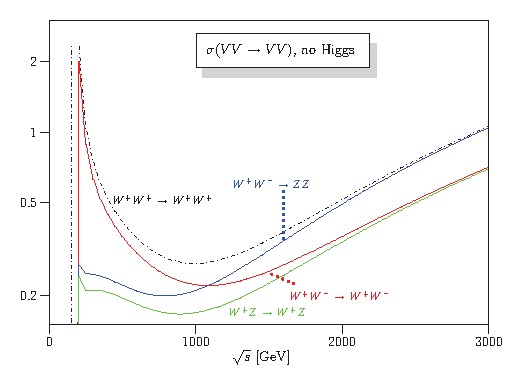
\includegraphics[height=.25\textheight]{figs/ssww_13tev/introduction/vbs_xsec_nohiggs}
  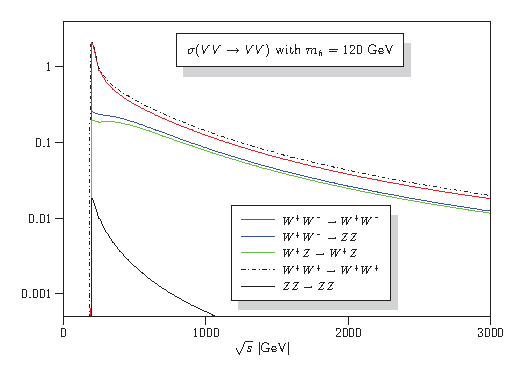
\includegraphics[height=.25\textheight]{figs/ssww_13tev/introduction/vbs_xsec_higgs120}
 
  \caption[Cross sections in nanobarns for five different scattering processes of longitudinally polarized vector bosons as a function of center of mass energy $\sqrt{s}$.  Without a SM Higgs boson (left), the cross sections grow unbounded with $\sqrt{s}$; however with a $120\gev$ Higgs boson (right), the cross sections no longer diverge.]{Cross sections in nanobarns for five different scattering processes of longitudinally polarized vector bosons as a function of center of mass energy $\sqrt{s}$.  Without a SM Higgs boson (left), the cross sections grow unbounded with $\sqrt{s}$; however with a $120\gev$ Higgs boson (right), the cross sections no longer diverge.  Plots taken from~\cite{2008.vbs-resonances-unitarity}.}
  \label{fig:ssww13tev_vbs_xsec_higgs}
\end{figure}

With the discovery of the Higgs boson in 2012~\cite{HIGG-2012-27, CMS-HIG-12-028}, the EWSB mechanism can now be directly studied.
Due to the exchange of a Higgs in the $s$- and $t$-channel VBS diagrams (\ssww itself only contains the $t$-channel diagram), VBS processes are directly sensitive to properties of the Higgs.
For example, the high-mass tail in the $VV$ scattering system allows an approximation of the effective coupling strength of the Higgs to vector bosons that is independent of any assumptions on the Higgs width~\cite{2015.higgs-constraints-from-vbs}.
Additionally, the center of mass energy dependence of the $VV$ scattering can reveal whether the Higgs boson unitarizes the longitudinal scattering amplitude fully or only partially~\cite{2014.higgs-WW-scattering-theory}.

VBS events are characterized by two quarks from the colliding protons each radiating a massive vector boson which then scatter and decay in the detector.
The incoming quarks carry a large amount of momentum and only deflect a small amount upon radiating the vector boson; as a result, they often travel very close to the beam line.
Ignoring the decay products of the bosons, these VBS events result in a final state of two vector bosons ($V$) and two jets ($j$) at high pseudorapidities (called \emph{forward jets}) from the outgoing quarks.
The shorthand $VVjj$ is used to represent this final state.

$VVjj$ events can be produced via two different physical processes.
The first involves purely electroweak interactions in the tree-level diagrams, with $\mathcal{O}(\alpha_{\textrm{EWK}}) = 6$ %(including the decays of the bosons).
and will be referred to as \emph{EWK production}.
This can be further broken down into VBS and non-VBS production.
In the VBS EWK production, the scattering occurs via triple or quartic gauge couplings, as well as the $s$- or $t$-channel exchange of a Higgs boson.
%These diagrams are shown in Figure~\ref{fig:ssww13tev_diagrams_vbs}.
The non-VBS EWK production contains the same final state of two vector bosons and two outgoing quarks, but the bosons do not scatter.
Due to gauge invariance, it is not possible to separate the VBS from the non-VBS productions~\cite{2006.isolating-vbs-lhc}; therefore, both are included in the signal generation and are indistinguishable from one another.
The second process involves a mix of the EWK and strong interactions, of order $\mathcal{O}(\alpha_s) = 2 \otimes \mathcal{O}(\alpha_{\textrm{EWK}}) = 4$ and will be referred to as \emph{QCD production}.
The tree-level Feynman diagrams for VBS EWK, non-VBS EWK, and QCD $VVjj$ production are found in Figures~\ref{fig:ssww13tev_diagrams_vbs}, \ref{fig:ssww13tev_diagrams_ewk}, and \ref{fig:ssww13tev_diagrams_qcd}, respectively.

\begin{figure}[htbp]
  \centering
  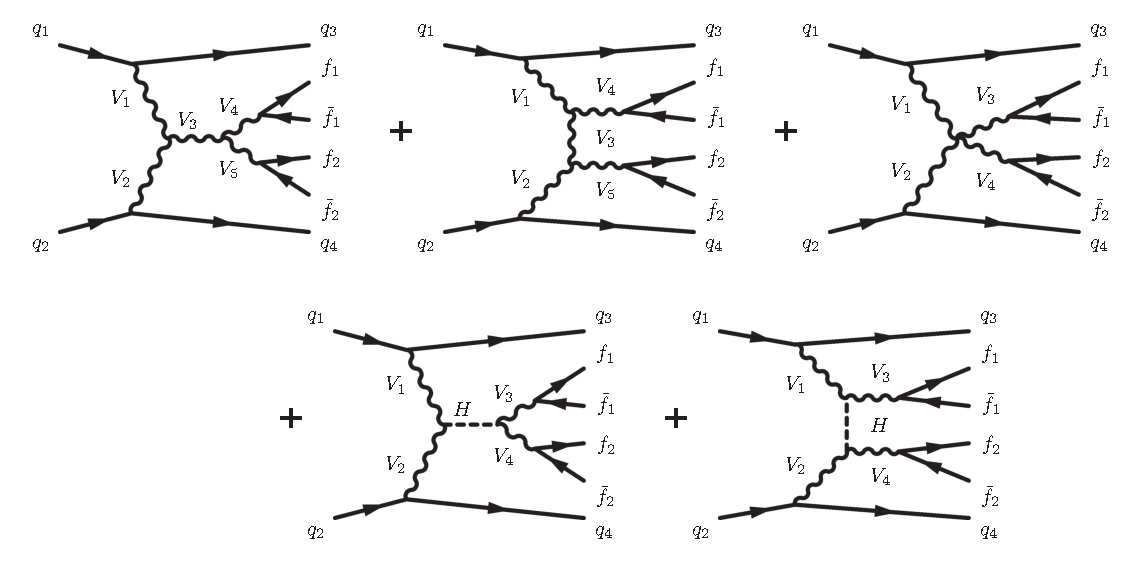
\includegraphics[width=.8\textwidth]{figs/ssww_13tev/diagrams/Vbscore}
  \caption{Tree-level Feynman diagrams for VBS EWK $VVjj$ production including triple gauge couplings involving $W$ and/or $Z$ bosons (top left and top middle), quartic gauge coupling (top right), or the exchange of a Higgs boson ($s$-channel bottom left and $t$-channel bottom right).  The labels are quarks ($q$), fermions ($f$), and gauge bosons ($V = W,Z$).}
  \label{fig:ssww13tev_diagrams_vbs}
\end{figure}

\begin{figure}[htbp]
  \centering
  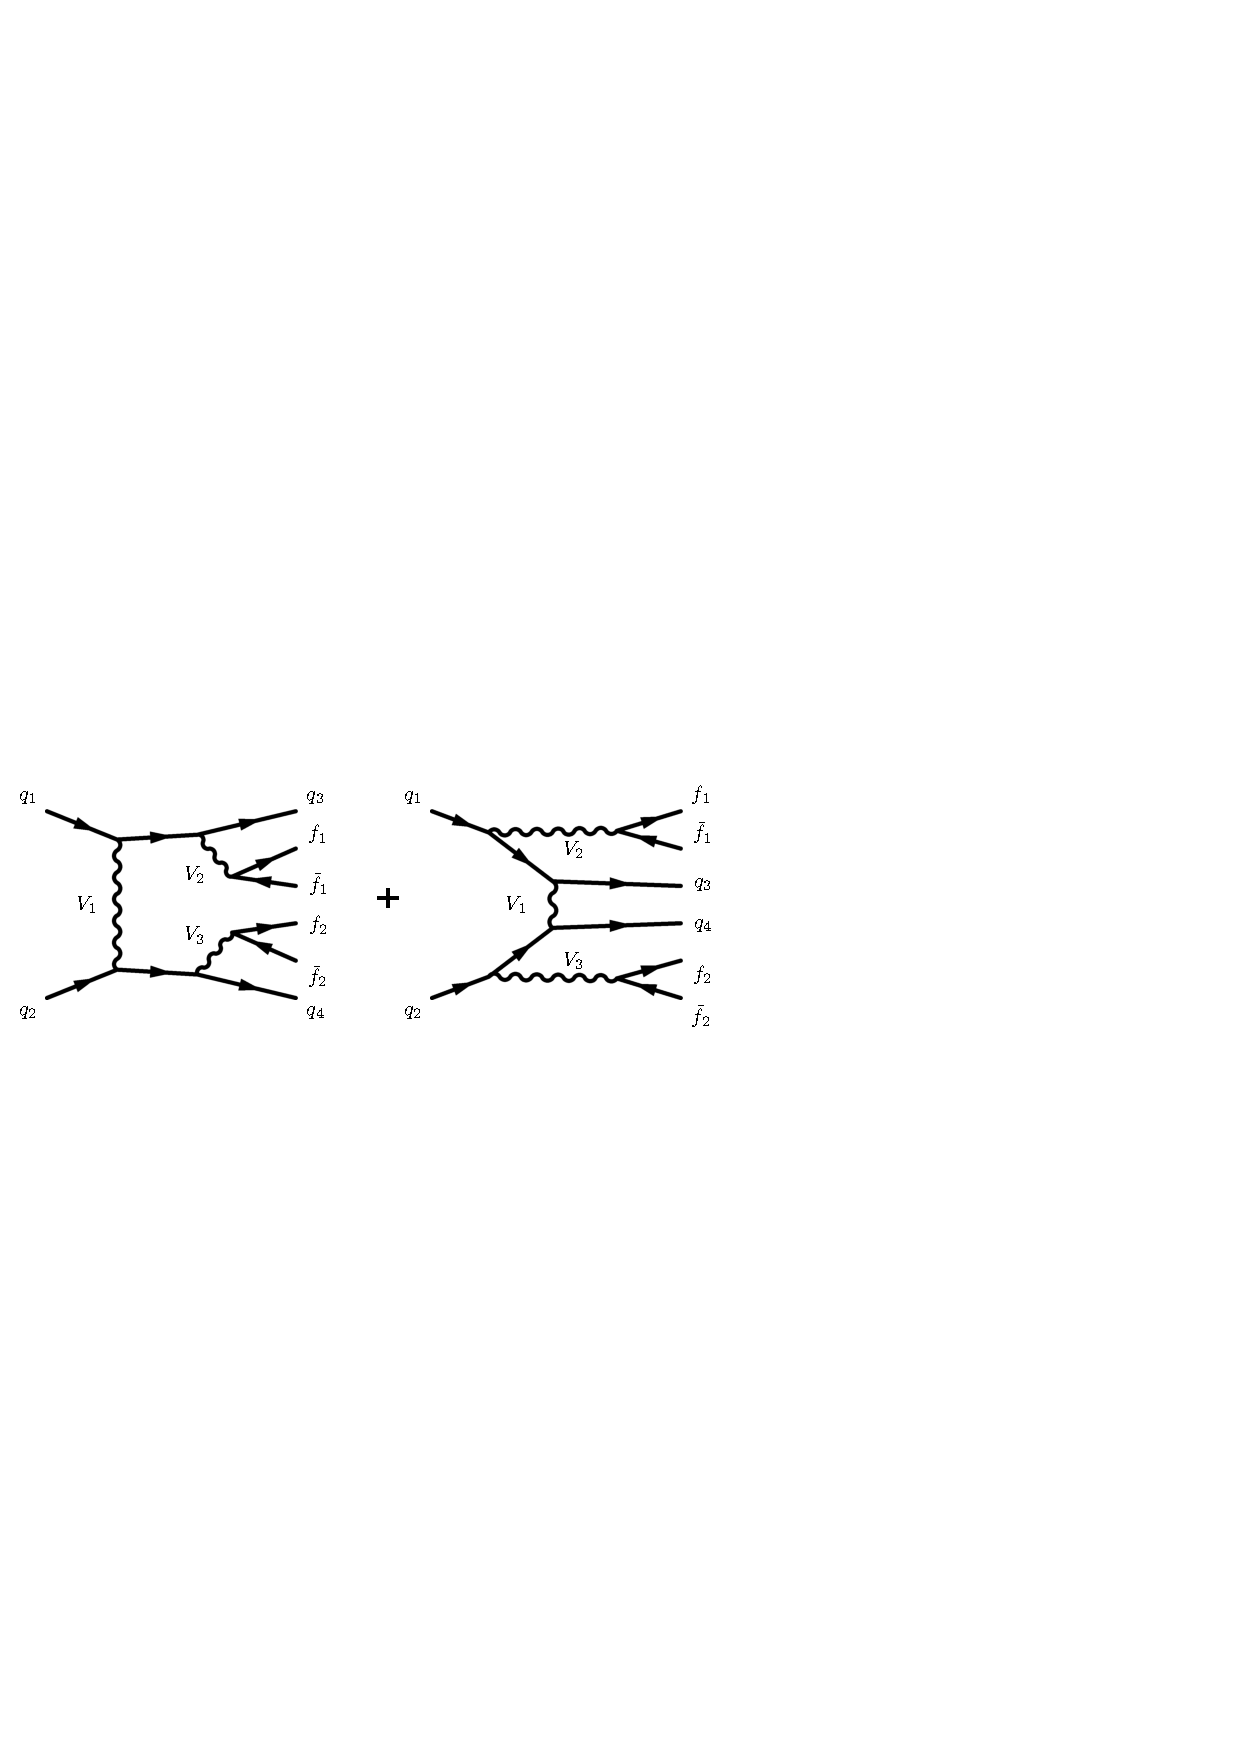
\includegraphics[width=.54\textwidth]{figs/ssww_13tev/diagrams/NoVbsEW}
  \caption{Tree-level Feynman diagrams for non-VBS EWK $VVjj$ production.  The labels are quarks ($q$), fermions ($f$), and gauge bosons ($V = W,Z$).}
  \label{fig:ssww13tev_diagrams_ewk}
\end{figure}

\begin{figure}[htbp]
  \centering
    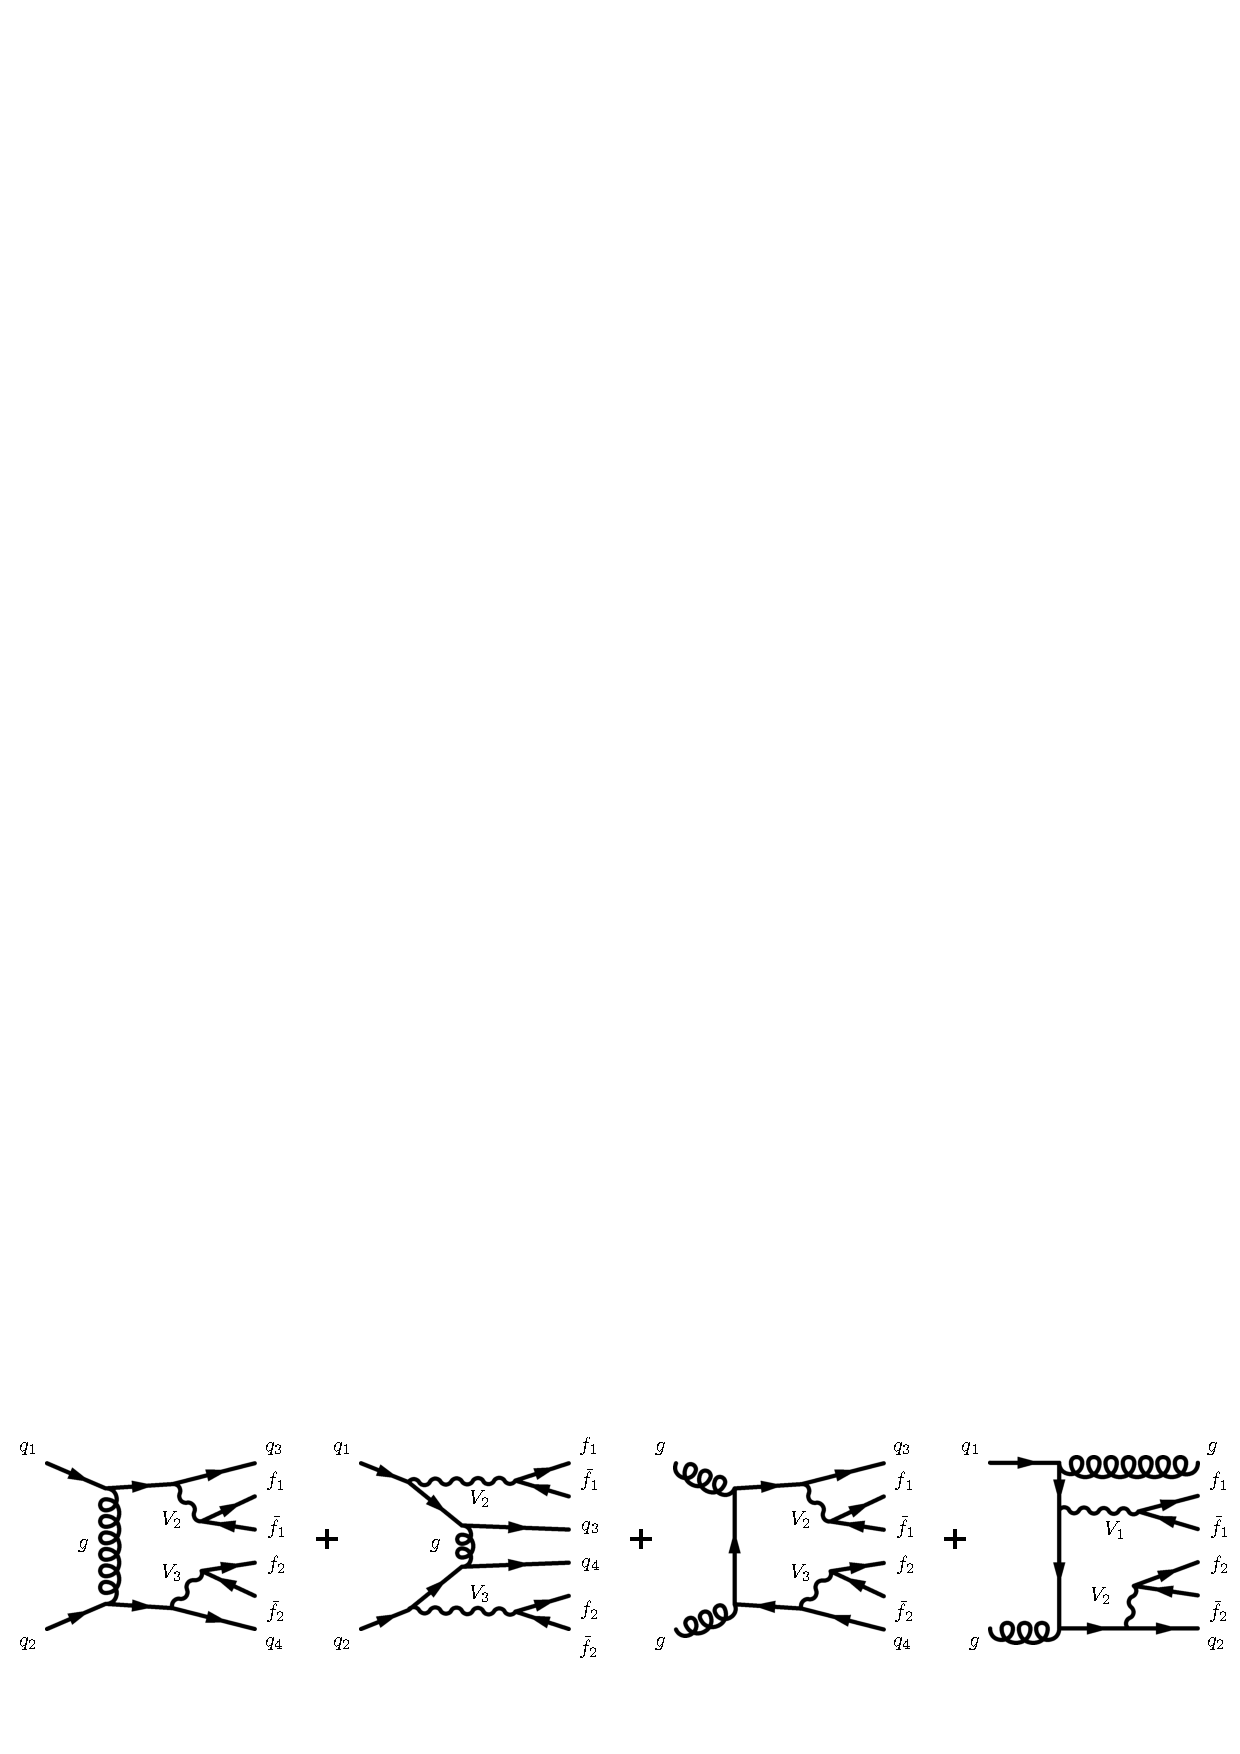
\includegraphics[width=\textwidth]{figs/ssww_13tev/diagrams/VbsQCD}
  \caption{Tree-level Feynman diagrams for QCD $VVjj$ production.  The labels are quarks ($q$), fermions ($f$), and gauge bosons ($V = W,Z$).}
  \label{fig:ssww13tev_diagrams_qcd}
\end{figure}

\subsection{Same-sign $W^{\pm}W^{\pm}$ scattering}\label{ssww13tev:ssww_topology}
Same-sign \ssww scattering is considered to be one of the best channels for studying VBS at the LHC~\cite{2015.higgs-constraints-from-vbs}.
This is due primarily to the ratio of the EWK to the QCD production, which matters a great deal due to the VBS events being a subset of the total EWK production.
In an analysis the EWK production would be conisdered the signal and the QCD production a background, so a favorable ratio of the two helps greatly when comparing the size of the signal to the backgrounds.
A study at \com{8}~\cite{2013.ssww-8tev-atlas-support} was done using the \tt{SHERPA} Monte Carlo (MC) generator to calculate EWK and QCD production cross sections at leading order for a variety of $VVjj$ processes decaying to leptons and can be found in Table~\ref{tab:ssww13tev_qcd_vs_ewk}.
Despite its lower cross section compared to other $VVjj$ processes, the EWK to QCD ratio for \ssww is approximately one-to-one, whereas for opposite-sign \oswwjj the ratio is closer to 3\%.

%There are several advantages to studying the same-sign $WW$ process specifically.
%The final state's net charge of $\pm 2$ helps considerably in reducing the number of background processes that can mimic the signal.

\begin{table}[htbp]
  \centering
  \begin{tabular}{l l r r}
    Process & Final state & $\sigma_{\textrm{EWK}}$ & $\sigma_{\textrm{QCD}}$ \\
    \hline\hline
    $W^{\pm}W^{\pm}$ & $l^{\pm}l^{\pm}\nu\nu jj$    & 19.5 fb & 18.8 fb \\
    $W^{\pm}W^{\mp}$ & $l^{\pm}l^{\mp}\nu\nu jj$    & 91.3 fb & 3030 fb \\
    $W^{\pm}Z$      & $l^{\pm}l^{\pm}l^{\mp}\nu jj$ & 30.2 fb & 687 fb  \\
    $ZZ$          & $l^{+}l^{-}\nu\nu jj$        & 2.4 fb  & 162 fb  \\
    $ZZ$          & $l^{+}l^{-}l^{+}l^{-} jj$     & 1.5 fb  & 106 fb \\
    \hline
  \end{tabular}
  \caption[Predicted cross sections for EQK and QCD production of diboson processes relevant to VBS at \com{8} using the \tt{SHERPA} MC generator.  Loose generator level cuts are applied on lepton $\pt > 5\gev$, dilepton invariant mass $m_{ll} > 4\gev$, and at least two jets with $m_{jj} > 10\gev$.]{Predicted cross sections for EQK and QCD production of diboson processes relevant to VBS at \com{8} using the \tt{SHERPA} MC generator.  Loose generator level cuts are applied on lepton $\pt > 5\gev$, dilepton invariant mass $m_{ll} > 4\gev$, and at least two jets with $m_{jj} > 10\gev$.  Numbers taken from~\cite{2013.ssww-8tev-atlas-support}.}
  \label{tab:ssww13tev_qcd_vs_ewk}
\end{table}

This analysis studies \ssww scattering where both $W$ bosons decay leptonically to $e\nu$ or $\mu\nu$\footnote{Throughout the rest of this chapter, $l$ denotes either electrons ($e$) or muons ($\mu$) unless stated otherwise.  Additionally, $e$, $\mu$, and $\nu$ (neutrino) with no charge or anti-particle designation refer interchangeably to either the particle or anti-particle.}.
The \ssww VBS final state consists of two leptons with the same electric charge, two neutrinos, and two high energy forward jets with a large invariant mass.
Tree-level Feynman diagrams of VBS \ssww production can be found in Figure~\ref{fig:ssww13tev_diagrams_vbs_ssww} and a visual representation of the VBS topology can be found in Figure~\ref{fig:ssww13tev_event_topology}.
The two forward jets also serve as a powerful tool to suppress the QCD production mode.
In EWK events, the two jets tend to have much higher separation and a larger combined invariant mass than the two leading jets in a QCD event.
The two plots shown in Figure~\ref{fig:ssww13tev_dijet_comparison} highlight the differences in these dijet quantities between the two production modes.
An ATLAS event display of a real \ssww candidate event is shown in Figure~\ref{fig:ssww13tev_event_display_mm}.

% i think i really only need to include the vbs diagrams for ssww (maybe also the ewk?) since the general VV ones are above for all processes
\begin{figure}[htbp]
  \centering
  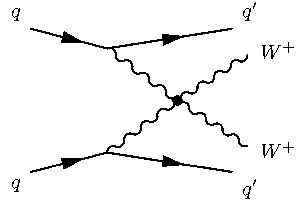
\includegraphics[width=.32\textwidth]{figs/ssww_13tev/diagrams/vbs1}
  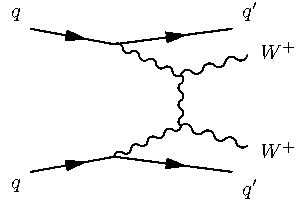
\includegraphics[width=.32\textwidth]{figs/ssww_13tev/diagrams/vbs2}
  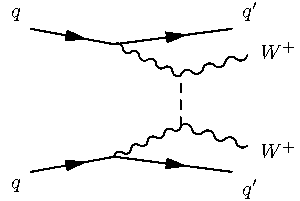
\includegraphics[width=.32\textwidth]{figs/ssww_13tev/diagrams/vbs3}
  \caption{Feynman diagrams for VBS EWK production of \ssww events. The leftmost diagram contains a quartic gauge coupling vertex, and the rightmost diagram contains an exchange of a Higgs boson. \TODO{Make diagrams consistent with others}}
  \label{fig:ssww13tev_diagrams_vbs_ssww}
\end{figure}

\begin{figure}[htbp]
  \centering
  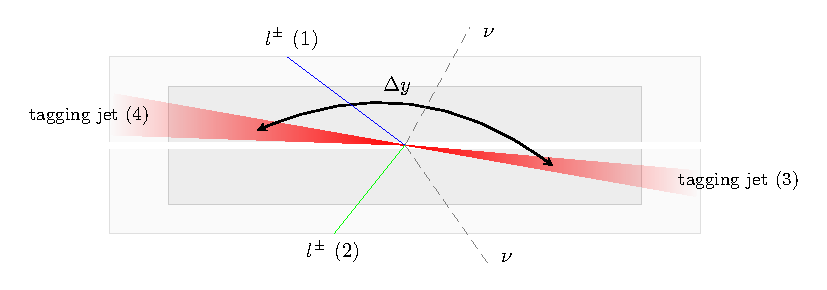
\includegraphics[width=.95\textwidth]{figs/ssww_13tev/introduction/vbs_event_topology}
  \caption{\ssww VBS event topology containing two leptons (1 and 2) with the same electric charge, two neutrinos, and two forward tagging jets (3 and 4) with large rapidity separation $\Delta y$.}
  \label{fig:ssww13tev_event_topology}
\end{figure}

\begin{figure}[htbp]
  \centering
  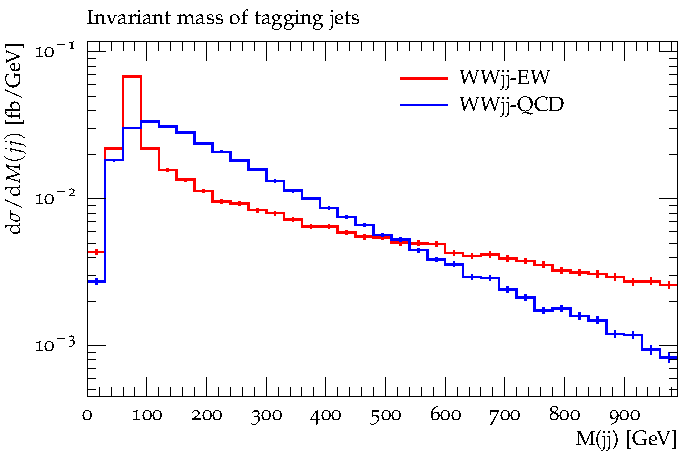
\includegraphics[width=.48\textwidth]{figs/ssww_13tev/introduction/Nm1_mjj}
  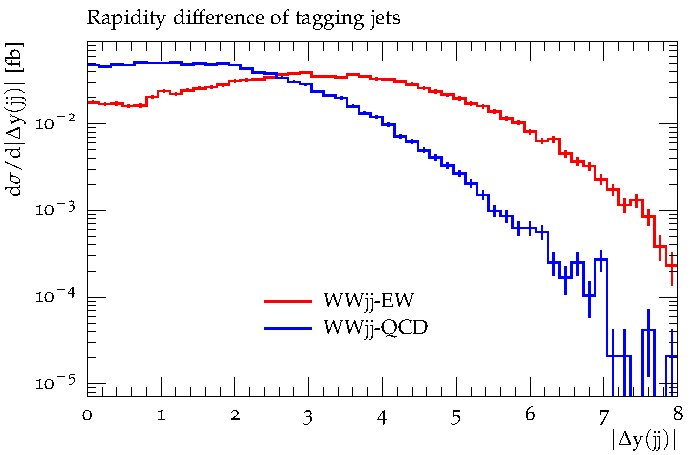
\includegraphics[width=.48\textwidth]{figs/ssww_13tev/introduction/Nm1_deltaY}
  \caption[Generator level comparisons at \com{8} of dijet invariant mass ($m_{jj}$, left) and dijet rapidity ($\Delta y_{jj}$, right) in EWK (red) and QCD (blue) \ssww events.  Both data sets have been normalized to the same area.]{Generator level comparisons at \com{8} of dijet invariant mass ($m_{jj}$, left) and dijet rapidity ($\Delta y_{jj}$, right) in EWK (red) and QCD (blue) \ssww events.  Both data sets have been normalized to the same area.  Plots taken from~\cite{2013.ssww-8tev-atlas-support}.}
  \label{fig:ssww13tev_dijet_comparison}
\end{figure}

\begin{figure}[htbp]
  \centering
  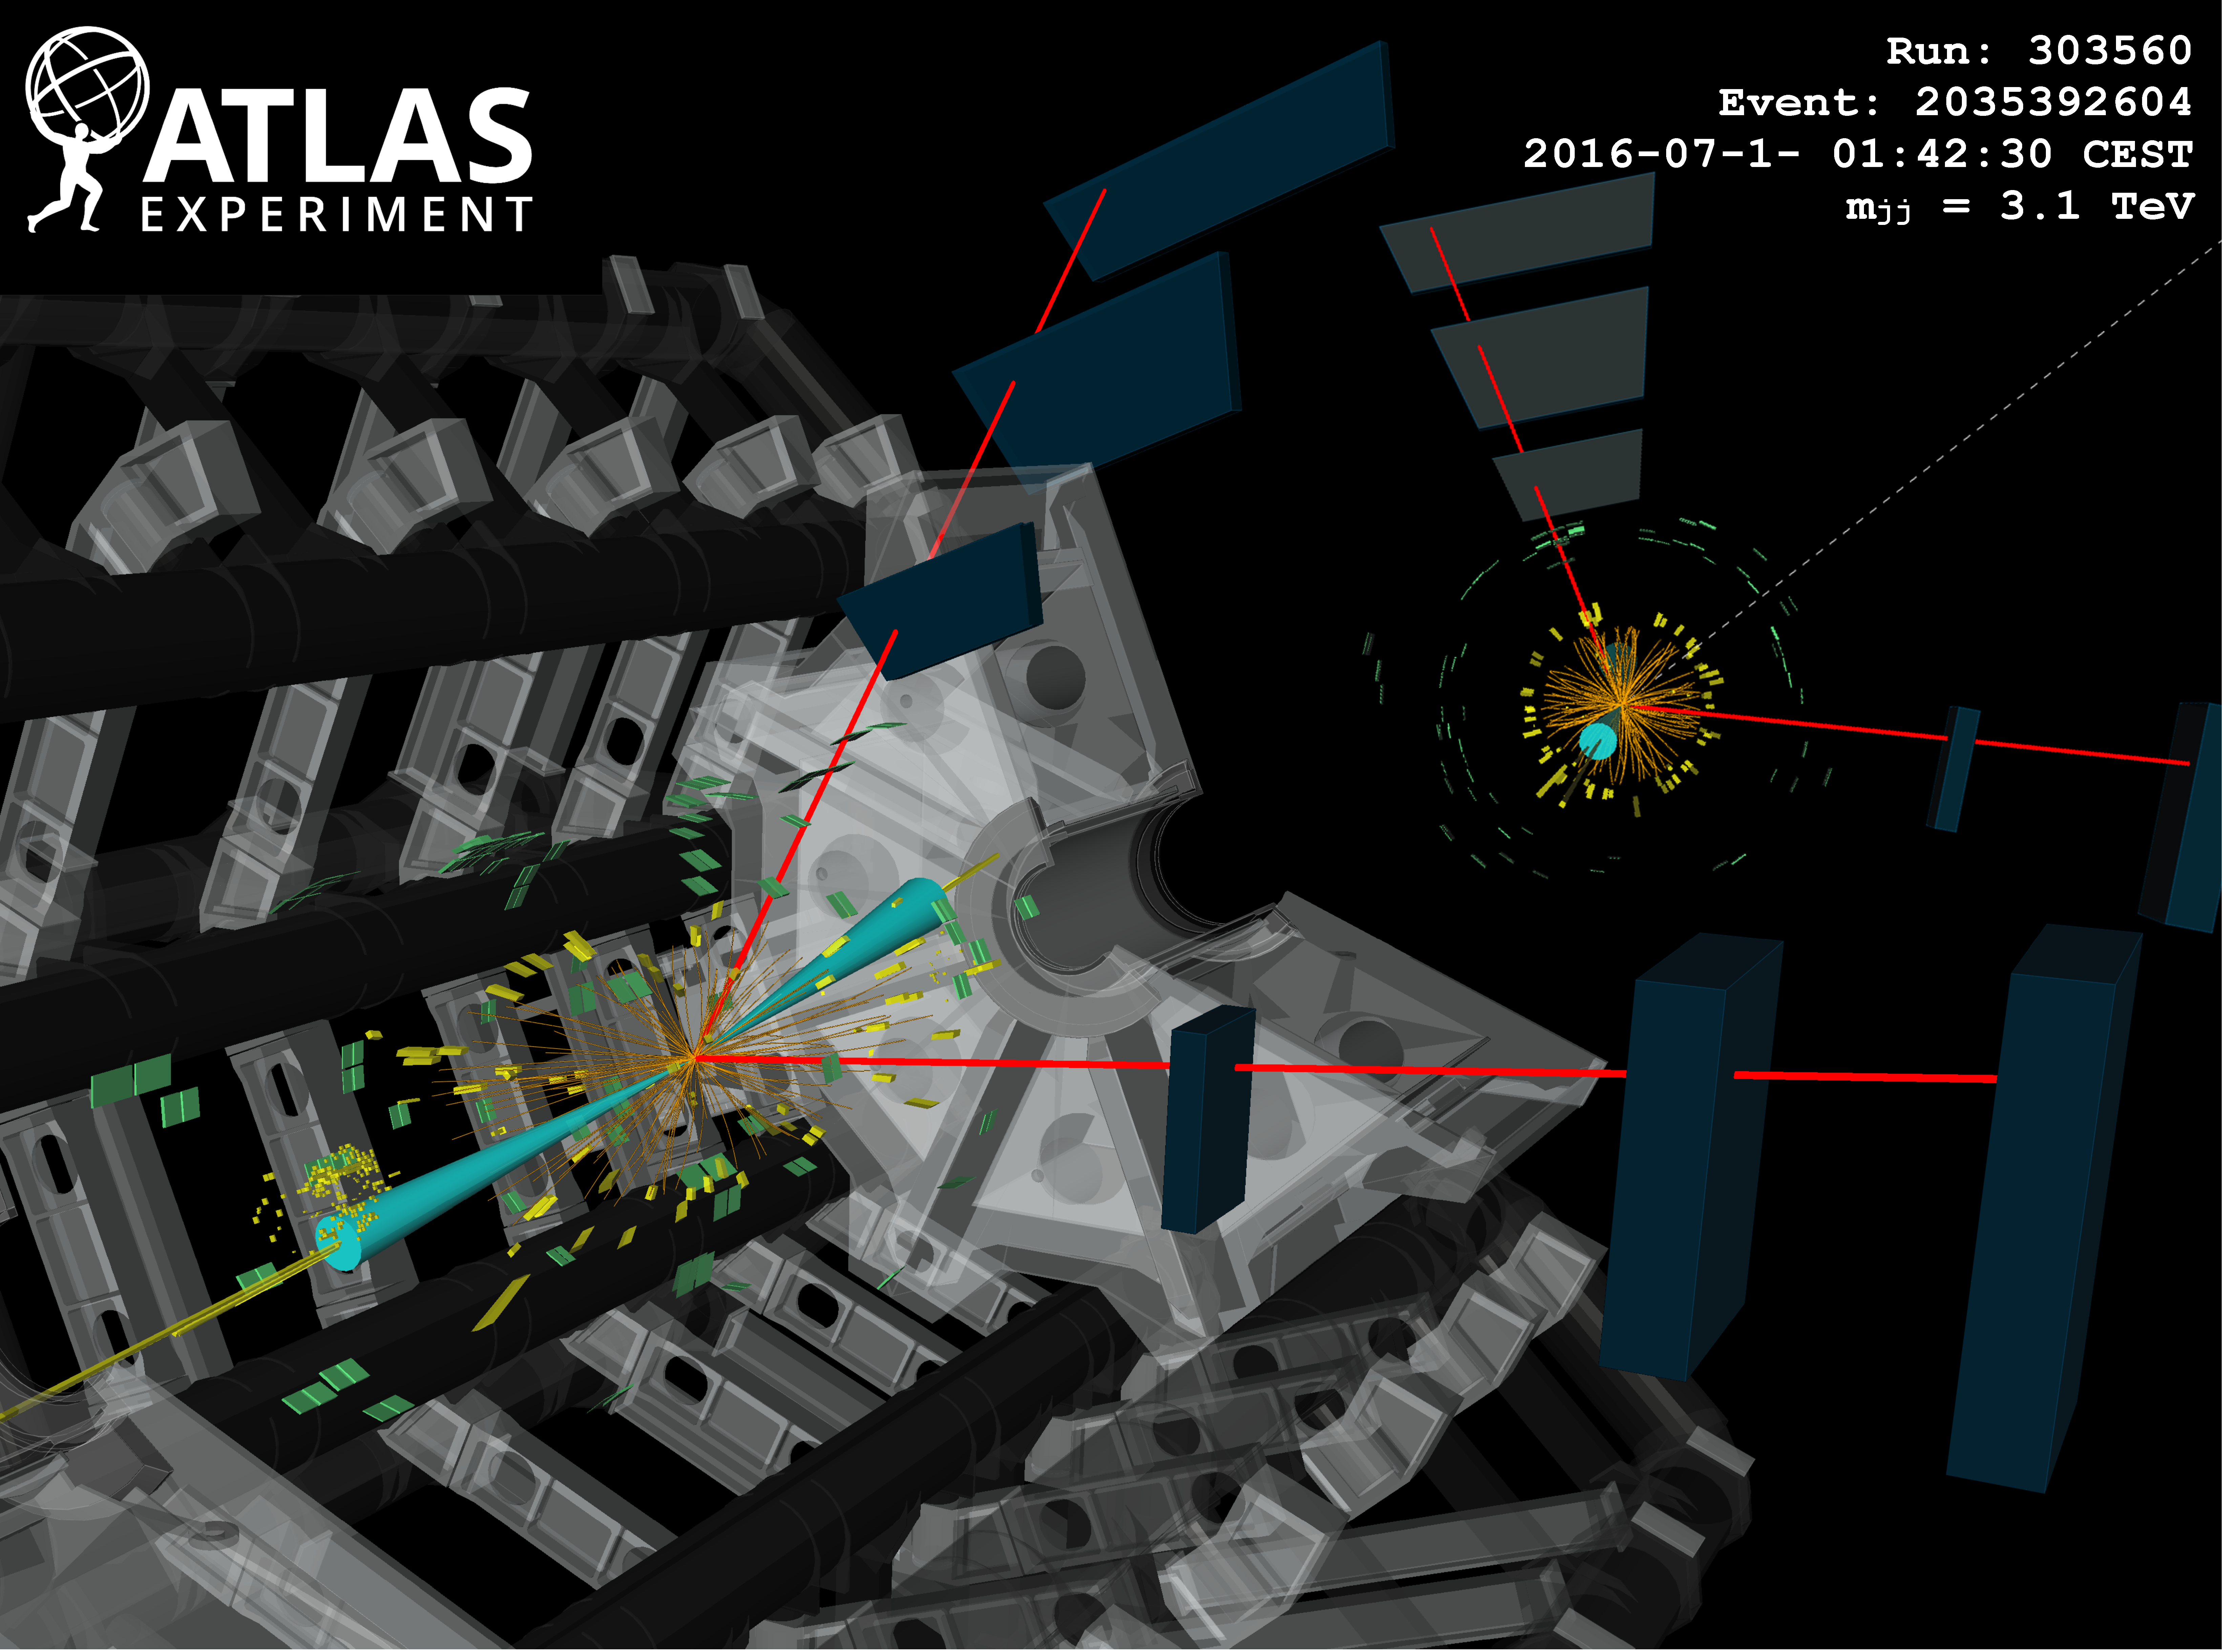
\includegraphics[width=.95\textwidth]{figs/ssww_13tev/introduction/evtdisplay_mm}
  \caption{ATLAS event display of a $pp\rightarrow W^{+}W^{+}\rightarrow\mu^{+}\nu_\mu\mu^{+}\nu_\mu jj$ event.  The muons are represented by the red lines travelling from the ID through the MS, and the forward jets are represented by the blue cones with yellow energy deposits in the calorimeters.  The direction of the $\met$ in the transverse plane is indicated by the gray dashed line in the inset image.  Event display taken from~\cite{2018.ssww-13tev-atlas-conf}.}
  \label{fig:ssww13tev_event_display_mm}
\end{figure}

\subsection{Overview of backgrounds}\label{ssww13tev:background_overview}
In addition to QCD production of \ssww events, there are several other processes that can end up with a final state of two same-sign leptons, two neutrinos, and two jets.
However, due to the $\pm 2$ final state charge, there is a considerable reduction in SM backgrounds (such as $Z$ boson events) when compared to an analysis like opposite-sign \oswwjj.

One of the largest sources of background involves processes with prompt leptons\footnote{Prompt leptons are those that are produced in the primary collision and are a direct decay product of the process of interest.  Non-prompt leptons originate from some secondary process, such as a $b$-hadron decay, or are jets that get mis-reconstructed as a lepton.}.
These are events that contain two leptons with the same electric charge and one or more additional leptons that are ``lost'', either by failing the selection criteria or falling outside of the detector's acceptance.
The number of processes that can contribute is limited by the requirement of same-sign leptons, and as a result this background is dominated by processes involving two or more vector bosons, with the largest contribution coming from $WZ$ events and smaller contributions from $ZZ$ and $t\bar{t}V$ events.
Triboson events where one boson decays hadronically also contribute to this background; however, the jets are generally softer and more central than in a typical VBS event, and the cuts applied on the forward jets suppress these contributions.

The other dominant background comes from non-prompt, or ``fake'', leptons.
Here one or more leptons originate from the decay of another particle unrelated to the signal process, such as a heavy-flavor decay or photon conversion, or come from a jet that is misidentified as a lepton.
This background is mostly made up of events from $t\bar{t}$ and $W$+jets processes, with a much smaller contribution from $V\gamma$ events. \TODO{check whether $V\gamma$ really qualifies as non-prompt, we lump $Z\gamma$ in with the charge flip background in the paper...}

Finally, opposite-sign lepton pairs can enter the signal region if one of the leptons is reconstructed with the wrong charge (called \emph{charge misidentification}\footnote{Charge misidentification is also referred to interchangeably as \emph{charge mis-ID} and \emph{charge flip}.}).
In practice, this only affects events with electrons, as the charge misidentification rate for muons is negligible~\cite{2013.muon-flip}.
This is a major background in events with two electrons, but is a much smaller contribution for events with one electron and one muon.

%\subsection{}\label{ssww13tev:theory}
%Hello world!



\section{Data and Monte Carlo samples}\label{ssww13tev:data_mc}
%\subsection{Data samples}\label{ssww13tev:data}
This analysis uses $36.1~\textrm{fb}^{-1}$ of \com{13} proton-proton collision data recorded by ATLAS during 2015 and 2016.
The uncertainty in the combined integrated luminosity is 2.1\%. It is derived following a methodology similar to that detailed in~\cite{2016.atlas-luminosity-8tev} and using the LUCID-2 detector for the baseline luminosity measurements \cite{2018.atlas-luminosity-lucid2} from calibration of the luminosity scale using $x$-$y$ beam-separation scans. % the TWIKI literally says I can copy these lines verbatim for papers/conf notes :D https://twiki.cern.ch/twiki/bin/view/Atlas/LuminosityForPhysics#2017_13_TeV_proton_proton_Morion

\subsection{Monte Carlo samples}\label{ssww13tev:mc}
A number of Monte Carlo (MC) simululations are employed to model signal and background processes.
In order to model the real collision data as closely as possible, each MC has been run through a full simulation of the ATLAS detector~\cite{2010.ATLAS-simulation-infrastructure} in \tt{GEANT4}~\cite{2003.GEANT4}, and events have been reconstructed using the same algorithms as the data.
The simulation reproduces as closely as possible the momentum resolutions and calorimeter responses of the detector, and also includes the effects of pileup by including soft QCD interactions using \pythiav{8.1}~\cite{2008.Pythia8}.
The MC samples used in this analysis are detailed in this section and summarized in Table~\ref{tab:ssww13tev_mcsamples}.

The \ssww samples are modeled using \sherpav{2.2.2}~\cite{2009.Sherpa, 2008.CS_Shower, 2009.METS} with the \nnpdf PDF set~\cite{2015.NNPDF3}.
The EWK signal samples are generated by fixing the electroweak coupling constant to $\mathcal{O}(\alpha_W) = 6$, and a QCD background sample was also generated with $\mathcal{O}(\alpha_W) = 4$.
\tt{SHERPA} includes up to one parton at next-to-leading order (NLO) and up to three at leading order (LO) in the strong coupling constant $\alpha_s$.
A second \ssww EWK sample is generated using \powhegbox{2}~\cite{2010.powhegbox} with the \nnpdf PDF set and at NLO accuracy.
This sample is only used for systematic studies, as \tt{POWHEG-BOX} does not include resonant triboson contributions in its matrix element, which are non-negligible at NLO~\cite{2018.ssww-scattering-at-lhc}.

Diboson processes ($VV$ where $V = W,Z$) are simulated with \sherpav{2.2.2} for mixed hadronic and leptonic decays and \sherpav{2.2.1} for fully leptonic decays of the bosons.
Similarly, triboson ($VVV$) and $V\gamma$ processes are simulated using \sherpav{2.1.1} with up to one parton at NLO and up to three at LO.
$W$+jets processes are simulated with \sherpa{2.2.1} with up to two partons at NLO and four at LO.
All the above \tt{SHERPA} samples use the \nnpdf PDF set and \tt{SHERPA}'s own parton showering.
The $Z$+jets events are generated with \mcatnlo~\cite{2014.madgraph_mcnlo} at LO and interfaced with \pythiav{8.1} for parton showering.

$t\bar{t}$ events are generated using \powhegbox{2} with the \ctten PDF set~\cite{2010.ct10}.
$t\bar{t}V$ samples are generated at NLO with \mcatnlo and the \nnpdf PDF set interfaced with \pythiav{8} for parton showering.
Finally, single top events are generated with \powhegbox{1} and the \tt{CT10f4} PDF set interfaced with \pythiav{6}~\cite{2006.Pythia6} for parton showering.

\begin{table}
  \centering
  \begin{tabular}{l l l}
    Process & Generator & Comments\\
    \hline\hline
    \ssww (EWK) & \sherpav{2.2.2} & Signal sample \\
    \ssww (EWK) & \powhegbox{2}   & Systematics sample \\
    \ssww (QCD) & \sherpav{2.2.2} & \\
    \hline
    \multirow{2}{*}{Diboson} & \sherpav{2.2.2} & Both bosons decay leptonically ($llll$, $lll\nu$, $ll\nu\nu$)\\
                             & \sherpav{2.2.1} & One boson decays leptonically, the other hadronically\\
    Triboson                 & \sherpav{2.1.1} & \\
    \hline
    $W$+jets           & \sherpav{2.2.1} & \\
    $Z$+jets           & \mcatnlo        & \\
    $V\gamma$          & \sherpav{2.1.1} & \\
    $V\gamma jj$ (EWK) & \sherpav{2.2.4} & \\
    \hline
    $t\bar{t}V$ & \mcatnlo        & \\
    $t\bar{t}$  & \powhegbox{2}   & \\
    Single top  & \powhegbox{1}   & EWK $t$-, $s$-, \& $Wt$-channels\\
    \hline
  \end{tabular}
  \caption{Summary of MC samples used in the analysis.}
  \label{tab:ssww13tev_mcsamples}
\end{table}


\section{Object and event selection}\label{ssww13tev:object_event_selection}
This section details the selection criteria for objects used in the analysis as well as the selection for signal events.

\subsection{Object selection}\label{ssww13tev:object_selection}
Muons, electrons, and jets all must pass strict selection requirements to ensure that only high quality, well measured objects are used.
For leptons, a baseline selection is defined (called the \emph{preselection}), which all leptons must pass in order to be considered for the analysis.
This preselection is an intentionally loose set of criteria designed to have high acceptance in order to reject backgrounds with additional leptons (i.e. $WZ\rightarrow 3l\nu jj$).
Signal leptons are then required to satisfy a much tighter \emph{signal selection} aimed at suppressing backgrounds from non-prompt or fake leptons.
A third set of lepton selection criteria, the \emph{loose selection}, defines a sample enriched in non-prompt leptons, and it is used in the fake-factor method for estimating the non-prompt background, discussed in detail in Section~\ref{ssww13tev:fake_factor}.
Jets are only required to pass one set of selection criteria.
These selections are detailed in the following sections and summarized in Table~\ref{tab:ssww13tev_muon_selection} for muons, Table~\ref{tab:ssww13tev_elec_selection} for electrons, and Table~\ref{tab:ssww13tev_jet_selection} for jets.

\subsubsection{Muon candidate selection}
Cuts on muon $\pt$ serve to reject low momentum leptons from background processes and additional collisions from pileup events.
Preselected muons must have transverse momentum $\pt > 6\gev$, and the signal muons must pass $\pt > 27\gev$.
The $\pt$ requirement for loose muons is lower than for signal muons, at $\pt > 15\gev$, for reasons that are discussed in Section~\ref{ssww13tev:ff_implementation}.
Muons are required to fall within the detector's $\eta$ acceptance: $|\eta| < 2.7$ for preselected muons, which is tightened to $|\eta| < 2.5$ for the signal muons.

Cuts on the transverse and longitudinal impact parameters are applied to ensure that the candidate muon originated from the primary particle interaction and not some other source, such as a heavy flavor decay.
The preselection and the loose selection both have relaxed requirements on the transverse impact parameter significance ($d_0/\sigma_{d_{0}}$) than the signal selection; all three have the same requirement on the transverse impact paramter ($|z_0\times\sin\theta|$).

Finally, the muon candidates are required to pass a particle identification and an isolation criteria as defined in~\cite{2016.muon-reconstruction-13tev}.
The methods used in constructing the identification and isolation working points are described in more detail in Section~\ref{detector:muon_reconstruction}.
The muon identification serves to select prompt muons with high efficiency and well measured momenta. % via the techniques detailed in Section~\ref{sec:reconstruction}.
This analysis uses two different working points: \tt{Loose} for preselected muons and \tt{Medium} for loose and signal muons, where \tt{Medium} muons are a tighter subset of those that pass the \tt{Loose} requirement.
Muon isolation is a measurement of detector activity around the muon candidate, and it is measured with both track-based and calorimeter-based variables.
The isolation working point used for the signal muons, \tt{Gradient}, is defined such that there is 90\% or better background rejection efficiency for $25\gev$ muons, and 99\% efficiency at $60\gev$.
There is no minimum isolation requirement for preselected or loose muons.
Loose muons are additionally required to fail one or both of the signal transverse impact parameter cut and signal isolation requirement.

\begin{table}[htbp]
  \centering
  \begin{tabular}{l l}
    \multicolumn{2}{c}{Muon preselection} \\ 
    \hline\hline
    Momentum cut                  & $\pt > 6~\textrm{GeV}$ \\
    Angular acceptance            & $|\eta| < 2.7$ \\
    Longitudinal impact parameter & $|z_0\times\sin\theta| < 0.5~\textrm{mm}$ \\
    Transverse impact parameter   & $d_0/\sigma_{d_{0}} < 10$ \\
    Particle identification       & \tt{Loose} \\
    \hline
  \end{tabular}

  \vspace{8mm}

  \begin{tabular}{l l}
    \multicolumn{2}{c}{Muon signal selection} \\ 
    \hline\hline
    Momentum cut                  & $\pt > 27~\textrm{GeV}$ \\
    Angular acceptance            & $|\eta| < 2.5$ \\
    Longitudinal impact parameter & $|z_0\times\sin\theta| < 0.5~\textrm{mm}$ \\
    Transverse impact parameter   & $d_0/\sigma_{d_{0}} < 3$ \\
    Particle identification       & \tt{Medium} \\
    Particle isolation            & \tt{Gradient}\\
    \hline
  \end{tabular}

  \vspace{8mm}

  \begin{tabular}{l l}
    \multicolumn{2}{c}{Muon loose selection} \\ 
    \hline\hline
    Momentum cut                  & $\pt > 27~\textrm{GeV}$ \\
    Angular acceptance            & $|\eta| < 2.5$ \\
    Longitudinal impact parameter & $|z_0\times\sin\theta| < 0.5~\textrm{mm}$ \\
    Transverse impact parameter   & $d_0/\sigma_{d_{0}} < 10$ \\
    Particle identification       & \tt{Medium} \\
    \multicolumn{2}{c}{Fail signal transverse impact parameter and/or isolation cuts} \\
    \hline
  \end{tabular}
  \caption{Muon selection criteria.  All muons are required to pass the preselection (top), and then either the signal (middle) or loose (bottom) criteria is applied to the preselected electrons.}
  \label{tab:ssww13tev_muon_selection}
\end{table}


\subsubsection{Electron candidate selection}
The electron candidate selections are very similar to those for muons.
The $\pt$ cut starts at $\pt > 6\gev$ for the preselection, increases to $\pt > 20\gev$ for loose electrons, and finally to $\pt > 27\gev$ for signal electrons.
The $|\eta|$ cut for electrons requires $|\eta| < 2.47$ for all electrons, with the region $1.37 \le |\eta| \le 1.52$ removed from loose and signal electrons.
This is where the electromagnetic calorimeter transitions from the barrel to the endcaps and is not fully instrumented.
Both the transverse and longitudinal impact parameter cuts are the same for all electron selections.

The electron particle identification uses a multivariate likelihood technique (LH) detailed in Section~\ref{detector:electron_reconstruction}.
Preselected electrons must pass the \tt{LooseLH} working point with an additional requirement that there be a reconstructed track hit in the first layer of the pixel detector (a so-called $B$-layer hit).
The LH requirement for the loose and signal electrons increases in tighness using \tt{MediumLH} and \tt{TightLH} electrons, respectively.
As for isolation, the \tt{Gradient} working point is required for signal electrons only.
The loose electrons must fail one or both of the signal identification and isolation requirements.

\begin{table}[htbp]
  \centering
  \begin{tabular}{l l}
    \multicolumn{2}{c}{Electron preselection} \\ 
    \hline\hline
    Momentum cut                  & $\pt > 6\gev$ \\
    Angular acceptance            & $|\eta| < 2.47$ \\
    Longitudinal impact parameter & $|z_0\times\sin\theta| < 0.5~\textrm{mm}$ \\
    Transverse impact parameter   & $d_0/\sigma_{d_{0}} < 5$ \\
    Particle identification       & \tt{LooseLH} + $B$-layer hit \\
    \hline
  \end{tabular}

  \vspace{8mm}

  \begin{tabular}{l l}
    \multicolumn{2}{c}{Electron signal selection} \\ 
    \hline\hline
    Momentum cut                  & $\pt > 27\gev$ \\
    Angular acceptance            & $|\eta| < 2.47$, excluding $1.37 \le |\eta| \le 1.52$ \\
    Longitudinal impact parameter & $|z_0\times\sin\theta| < 0.5~\textrm{mm}$ \\
    Transverse impact parameter   & $d_0/\sigma_{d_{0}} < 5$ \\
    Particle identification       & \tt{TightLH} \\
    Particle isolation            & \tt{Gradient}\\
    \hline
  \end{tabular}

  \vspace{8mm}

  \begin{tabular}{l l}
    \multicolumn{2}{c}{Electron loose selection} \\ 
    \hline\hline
    Momentum cut                  & $\pt > 20\gev$ \\
    Angular acceptance            & $|\eta| < 2.47$, excluding $1.37 \le |\eta| \le 1.52$ \\
    Longitudinal impact parameter & $|z_0\times\sin\theta| < 0.5~\textrm{mm}$ \\
    Transverse impact parameter   & $d_0/\sigma_{d_{0}} < 5$ \\
    Particle identification       & \tt{MediumLH} \\
    \multicolumn{2}{c}{Fail signal identification and/or isolation cuts} \\
    \hline
  \end{tabular}
  \caption{Electron selection criteria.  All electrons are required to pass the preselection (top), and then either the signal (middle) or loose (bottom) criteria is applied to the preselected electrons.}
  \label{tab:ssww13tev_elec_selection}
\end{table}


\subsubsection{Jet candidate selection}
The final objects that need to pass selection are jets.
Jets are clustered using the anti-$k_t$ algorithm~\cite{2008.antikt} within a radius of $\deltar = 0.4$.
The jets are then calibrated using $E_\textrm{T}$- and $\eta$-dependent correction factors that are trained using MC simulations~\cite{2017.jet-energy-scale-13tev}.
The calibrated jets are required to have $\pt > 30\gev$ if they lie in the forward regions of the detector ($2.4 < |\eta| < 4.5$) and $\pt > 25\gev$ in the central region ($|\eta| \le 2.4$).
In order to suppress pileup jets, the so-called jet-vertex-tagger (JVT) discriminant associates a jet with the primary interaction vertex~\cite{2014.jet-vertex-tagger}; central jets with $\pt > 60\gev$ are required to pass the \tt{Medium} JVT working point, which corresponds to an average efficiency of over 92\%. %the exact value is JVT > 0.59 per https://twiki.cern.ch/twiki/bin/view/AtlasProtected/JVTCalibration#Working_points
Finally, the jets are required to be separated from the selected leptons by at least $\deltar(j,l) > 0.3$.

\begin{table}[htbp]
  \centering
  \begin{tabular}{l l}
    \multicolumn{2}{c}{Jet selection} \\ 
    \hline\hline
    \multirow{2}{*}{Momentum cut} & $\pt > 30\gev$ for $2.4 < |\eta| < 4.5$ \\
                                  & $\pt > 60\gev$ for $|\eta| < 2.4$ \\
    JVT cut                       & \tt{Medium}\\
    Jet-lepton separation         & $\deltar(j,l) > 0.3$ \\
    \hline
  \end{tabular}
  \caption{Jet selection criteria.  All jets are required to pass the above selection in order to be used in the analysis.}
  \label{tab:ssww13tev_jet_selection}
\end{table}

\subsubsection{Treatment of overlapping objects}\label{ssww13tev:overlap_removal}
In the event that one or more objects are reconstructed very close to each other, there is the possiblity for double-counting if both originated from the same object.
The procedure by which this ambiguity is resolved is called \emph{overlap removal} (OR).
The standard ATLAS recommendation for OR~\cite{2014.atlas-overlap-removal, 2018.atlas-wboson-top} is implemented in this analysis and is summarized in Table~\ref{tab:ssww13tev_or}.

Since electrons leave a shower in the EM calorimeter, every electron has a jet associated with it.
Therefore, any jets close to an electron (within $\deltar(e,j) < 0.2$) are rejected due to the high probability that they are the same object.
On the other hand, when jets and electrons overlap within a larger radius of $0.2 < \deltar(e,j) < 0.4$, it is likely that the electron and jet both are part of a heavy-flavor decay, and the electron is rejected.

High energy muons can produce photons via bremsstrahlung radiation or collinear final state radiation which result in nearby energy deposits in the calorimeters.
Non-prompt muons from hadronic decays produce a similar signature; however, in this case the jet has a higher track multiplicity in the ID.
It is possible to address both cases simultaneously by rejecting the jet when the ID track multiplicity is less than three---and otherwise rejecting the muon---for jets and muons within $\deltar(\mu,j) < 0.4$.

In addition to the case above where muon bremsstrahlung results in a nearby reconstructed jet, the ID track from the muon and the calorimeter energy deposit can lead to it being reconstructed as an electron.
In this case, if both a muon and an electron share a track in the ID, the muon is kept and the electron is rejected, unless the muon is calorimeter-tagged\footnote{A calorimeter-tagged (CT) muon is a muon that is identified by matching an ID track to a calorimeter energy deposit.  CT muons have relatively low reconstruction efficiency compared to those measured by the MS, but can be used to recover acceptance in regions of the detector where the MS does not have full coverage~\cite{2016.muon-reconstruction-13tev}.}, in which case the muon is removed in favor of the electron.

\begin{table}[htbp]
  \centering
  \begin{tabular}{l l l}
    Overlap         & Check & Result (remove $\rightarrow$ keep) \\
    \hline\hline
    \multirow{2}{*}{Electron \& Jet}  & $\deltar(e,j) < 0.2$       & Jet $\rightarrow$ Electron \\
                                      & $0.2 < \deltar(e,j) < 0.4$ & Electron $\rightarrow$ Jet \\
    \hline
    \multirow{2}{*}{Muon \& Jet}      & $\deltar(\mu,j) < 0.4$ and Jet $N_{\textrm{ID\ tracks}} < 3$
                                                                   & Jet $\rightarrow$ Muon \\
                                      & $\deltar(\mu,j) < 0.4$ and Jet $N_{\textrm{ID\ tracks}} \ge 3$
                                                                   & Muon $\rightarrow$ Jet \\
    \hline
    \multirow{2}{*}{Electron \& Muon} & Shared ID track            & Electron $\rightarrow$ Muon \\
                                      & Shared ID track \& muon is calo-tagged
                                                                   & Muon $\rightarrow$ Electron \\
    \hline
  \end{tabular}
  \caption{Summary of the overlap removal procedure used in the analysis.  If the criteria in the ``check'' column is met, in the ``result'' column, the object on the left of the arrow is removed in favor of the object on the right.}
  \label{tab:ssww13tev_or}
\end{table}

\subsection{Signal event selection}\label{ssww13tev:event_selection}
After the objects have been selected, cuts are applied on a per-event level to select \ssww signal events.
The event selection is summarized in Table~\ref{tab:ssww13tev_event_selection}. % and is detailed in this section.
%It includes the results of an optimization performed using a multidimensional grid scan.

The initial event selection chooses events that pass one or more of the trigger requirements listed in Table~\ref{tab:ssww13tev_triggers}.
At least one signal lepton is ``matched'' to a passed trigger in order to ensure that it was indeed a signal lepton that fired the trigger.
A collection of \emph{event cleaning} cuts must also be passed in order to remove events collected during periods in which one or more components of the detector was not operating optimally.
Finally, the events are required to contain at least one interaction vertex.
An event can have multiple reconstructed vertices from additional proton-proton collisions that occurred in the same bunch crossing.
In this case, the \emph{primary vertex} is determined by choosing the vertex with the largest sum of the $\pt^2$ of its associated tracks.

\begin{table}[htbp]
  \centering
  \begin{tabular}{l | c | c}
    & 2015 data & 2016 data \\
    \hline\hline
    \multirow{3}{*}{Electrons} & $\pt > 24\gev$ and \tt{Medium} ID & $\pt > 26\gev$ and \tt{Tight} ID and \tt{Loose} isolation\\
                               & $\pt > 60\gev$ and \tt{Medium} ID & $\pt > 60\gev$ and \tt{Medium} ID \\
                               & $\pt > 120\gev$ and \tt{Loose} ID & $\pt > 140\gev$ and \tt{Loose} ID \\
    \hline
    \multirow{2}{*}{Muons}     & $\pt > 20\gev$ and \tt{Loose} isolation & $\pt > 26\gev$ and \tt{Medium} isolation\\
                               & $\pt > 50\gev$ & $\pt > 50\gev$ \\
    \hline
  \end{tabular}
  \caption{Summary of trigger requirements for electrons and muons for \com{13} data collected in 2015 and 2016.  At least one of the triggers must be satisfied.}
  \label{tab:ssww13tev_triggers}
\end{table}

Events are then required to contain exactly two signal leptons with the same electric charge.
The dilepton pair must have a combined invariant mass of $m_{ll} \ge 20\gev$ in order to suppress low mass Drell-Yan backgrounds.
Two additional selections are applied to events in the $ee$-channel: both electrons are required to have $|\eta| < 1.37$ with an invariant mass at least $15\gev$ away from the $Z$-boson mass to reduce events where one electron is reconstructed with the wrong charge (this background will be discussed in more detail in Section~\ref{ssww13tev:charge_misid}).
To suppress backgrounds from final states with more than two leptons, such as $WZ$ or $ZZ$, events with more than two leptons passing the preselection are vetoed.

Missing transverse energy ($\met$) represents any particles that escape the detector without being measured, such as neutrinos, and it is defined as the magnitude of the vector sum of transverse momenta of all reconstructed objects.
It can be difficult to calculate accurately, as it involves measurements from all subsystems within the detector, and it is sensitive to any corrections that may be applied to the reconstructed physics objects~\cite{2018.met-13tev}.
These corrections, including the momentum smearing for muons, energy scale and smearing for electrons, and jet calibrations, are propagated to the $\met$ calculation.
Events are required to contain $\met > 30\gev$ in order to account for the two neutrinos from the $W$ boson decays.

At least two jets are required.
The leading and subleading jets must have $\pt > 65\gev$ and $\pt > 35\gev$, respectively, and are referred to as the \emph{tagging jets}.
Events are vetoed if they contain one or more jets that have been tagged as a $b$-jet to suppress backgrounds from heavy flavor decays (especially top quark events).
The $b$-tagging algorithm used by ATLAS is a boosted decision tree (BDT) called MV2c10, and this analysis uses a working point with 85\% efficiency~\cite{2018.btag-efficiency-13tev}.

Finally, cuts are applied on the VBS signature outlined in Section~\ref{ssww13tev:ssww_topology}.
The tagging jets are required to have a dijet invariant mass $m_{jj} > 200\gev$ and be separated in rapidity by $|\Delta y_{jj}| > 2.0$.
This preferentially selects the VBS EWK events over the QCD-produced \ssww events.

\begin{table}[htbp]
  \centering
  \begin{tabular}{l | l}
    \multicolumn{2}{c}{Event selection} \\
    \hline\hline
    \multirow{3}{*}{Event preselection} & Pass at least one trigger with a matched lepton \\
                                        & Pass event cleaning \\
                                        & At least one reconstructed vertex\\
    \hline
    \multirow{5}{*}{Lepton selection}   & Exactly two leptons passing signal selection \\
                                        & Both signal leptons with the same electric charge \\
                                        & Dilepton mass $m_{ll} > 20\gev$ \\
                                        & $|\eta| < 1.37$ and $|M_{ee} - M_Z| > 15\gev$ ($ee$-channel only) \\
                                        & Veto events with more than two preselected leptons \\
    \hline
    Missing transverse energy           & $\met \ge 30\gev$\\
    \hline
    \multirow{6}{*}{Jet selection}      & At least two jets \\
                                        & Leading jet $\pt > 65\gev$ \\
                                        & Subleading jet $\pt > 35\gev$\\
                                        & $m_{jj} > 200\gev$ \\
                                        & $N_{b\textrm{-jet}} = 0$ \\ %$b$-jet veto \\
                                        & $|\Delta y_{jj}| > 2.0$ \\
    \hline
  \end{tabular}
  \caption{The signal event selection.}
  \label{tab:ssww13tev_event_selection}
\end{table}


%\section{Signal definition}\label{ssww13tev:signal}
%Hello world!


\section{Background estimations}\label{ssww13tev:background}
The major sources of background events are summarized in Section~\ref{ssww13tev:background_overview}, and the methods used to estimate them are detailed in this section.  
Prompt backgrounds from $ZZ$ and $t\bar{t}+V$ are estimated directly from MC simulations.
The shape of the $WZ$ and $V\gamma$ backgrounds are taken from MC, and the predicted yeilds are normalized to the data predictions in dedicated control regions, as outlined in Sections~\ref{ssww13tev:wz} and \ref{ssww13tev:wgamma}, respectively.
Opposite sign events with a charge misidentified electron are estimated by a data-driven background method which is summarized in Section~\ref{ssww13tev:charge_misid}.
Finally, a \emph{fake-factor} method is used to estimate the contributions from non-prompt backgrounds and is the subject of Section~\ref{ssww13tev:fake_factor}.

\subsection{Estimation of the $WZ$ background}\label{ssww13tev:wz}
The dominant background involving prompt leptons comes from $WZ$+jets events.
The contribution is estimated from MC simulation and normalized to data in a control region enriched in $WZ$ events.
This region is defined by the same event selection as the signal region in Table~\ref{tab:ssww13tev_event_selection}, with the following changes applied to increase the purity of the $WZ$ process:
\begin{itemize}
\item The third lepton veto is inverted, requiring a third lepton with $\pt > 15\gev$
\item Two of the leptons must make a same-flavor opposite-sign pair. If more than one pair exists, the one with $m_{ll}$ closest to the $Z$ boson mass is chosen.
\item The trilepton invariant mass is required to be $m_{lll} > 106\gev$ to reduce contributions from $Z\gamma$ and $Z$+jets
\end{itemize}

Once the event yields in the control region are calculated, they are propagated to the final signal region fit, detailed in Section~\ref{ssww13tev:xsec_fit_method}, in a single bin combining all the lepton channels.
The systematic uncertainties of the $WZ$ background are also calculated at this time.
The event yields for the $WZ$ control region are listed in Table~\ref{tab:ssww13tev_wzcr_yields}, and distributions of the leading lepton $\pt$ and $\eta$ as well as trilepton invariant mass $m_{lll}$ are found in Figures~\ref{fig:ssww13tev_wzcr_lep0} and \ref{fig:ssww13tev_wzcr_mlll}, respectively.

\begin{table}[htbp]
  \centering
  \begin{tabular}{l r}
    \multicolumn{2}{c}{Event yields in the $WZ$ control region} \\
    \hline\hline
    $WZ$     & $197.9\pm 1.4$ \\
    $ZZ$     & $14.1\pm 0.3$ \\
    Triboson & $1.26\pm 0.1$ \\
    top      & $10.8\pm 1.1$ \\
    $Z\gamma$& $3.1\pm 1.1$ \\
    $Z$+jets & $2.5\pm 1.4$ \\
    \hline
    Total prediction & $229.7\pm 2.5$ \\
    Data             & $201 \pm 14.2$ \\
    \hline
  \end{tabular}
  \caption{Event yields in the $WZ$ control region before normalization.  All lepton flavor channels are combined.}
  \label{tab:ssww13tev_wzcr_yields}
\end{table}

\begin{figure}[htbp]
  \centering
  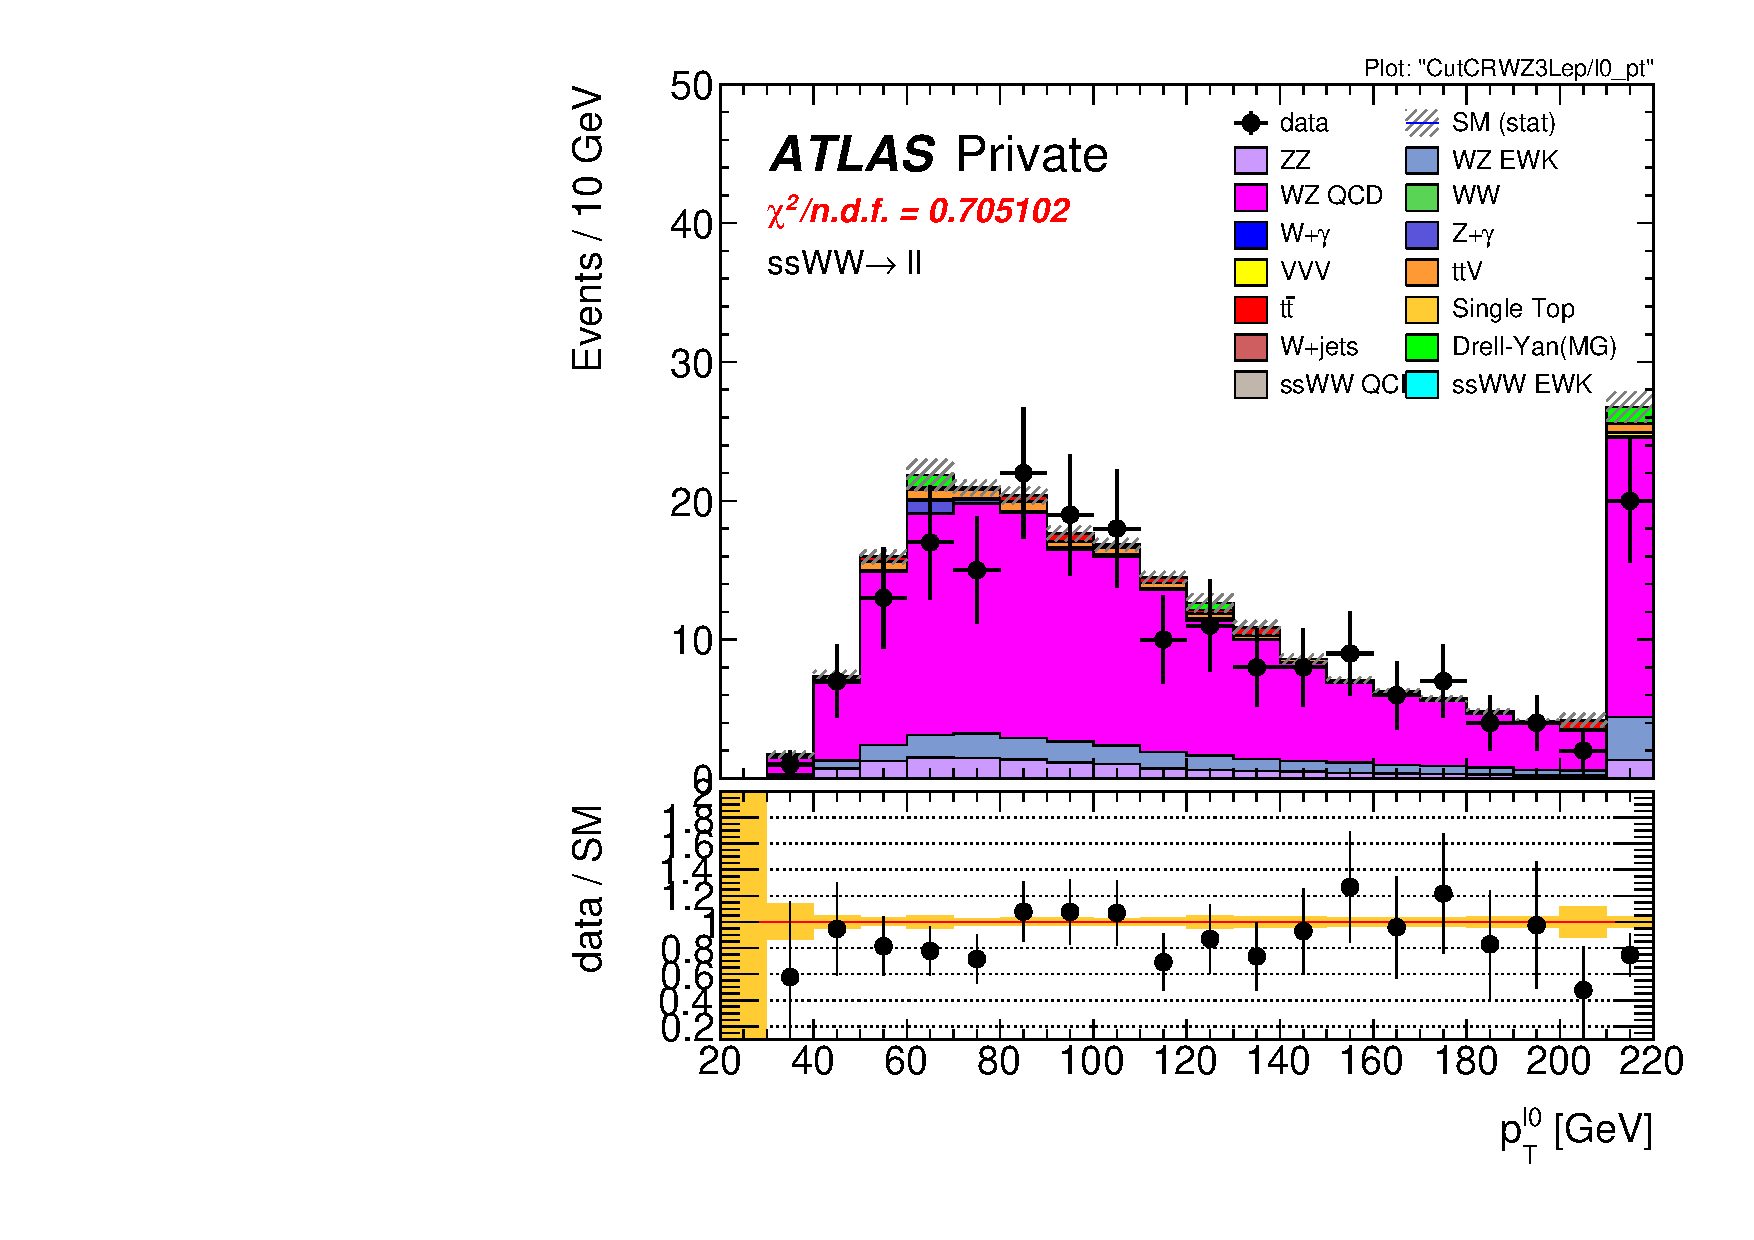
\includegraphics[width=.48\textwidth]{figs/ssww_13tev/backgrounds/wz/ll-CutCRWZ3Lep-l0_pt-lin}
  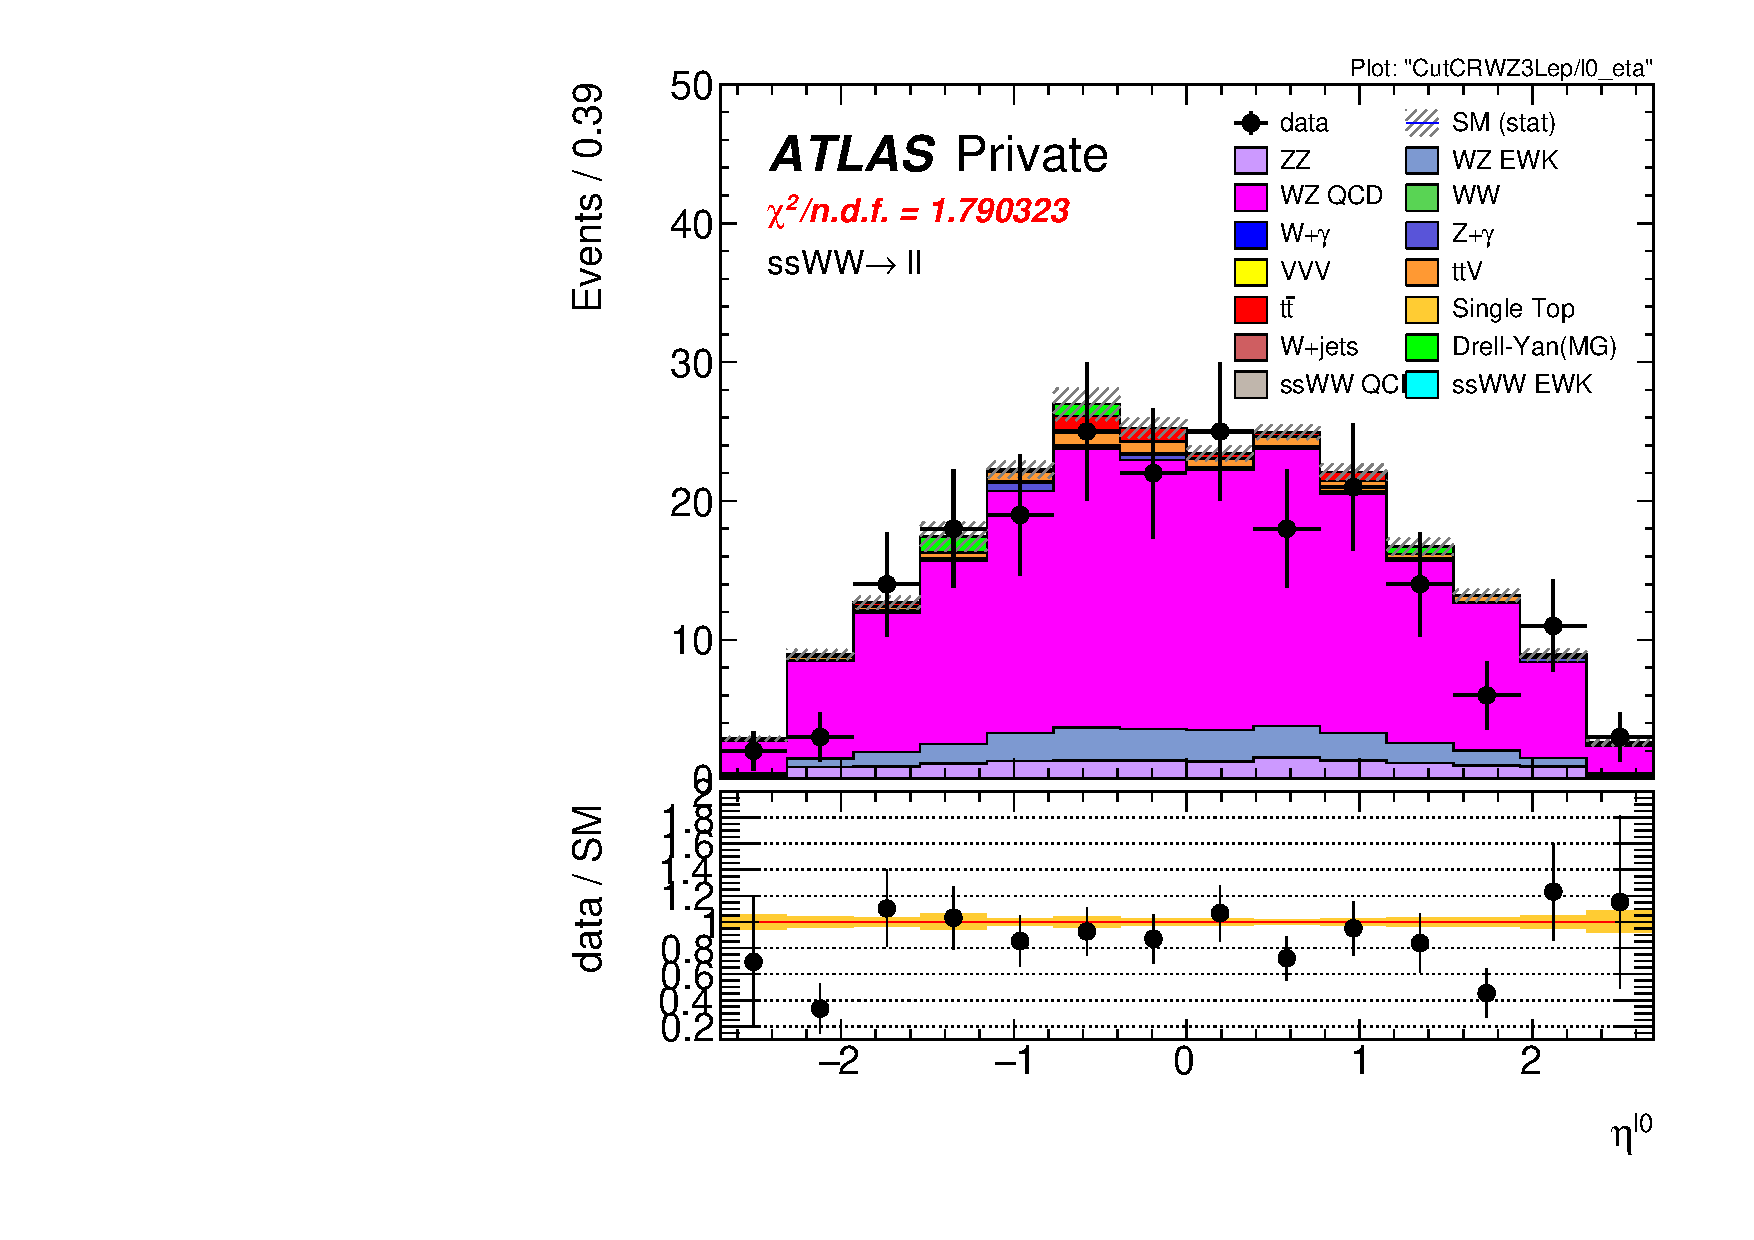
\includegraphics[width=.48\textwidth]{figs/ssww_13tev/backgrounds/wz/ll-CutCRWZ3Lep-l0_eta-lin}
  \caption{Leading lepton $\pt$ (left) and $\eta$ (right) distributions in the $WZ$ control region before normalization.  All lepton channels are combined.}
  \label{fig:ssww13tev_wzcr_mlll}
\end{figure}

\begin{figure}[htbp]
  \centering
  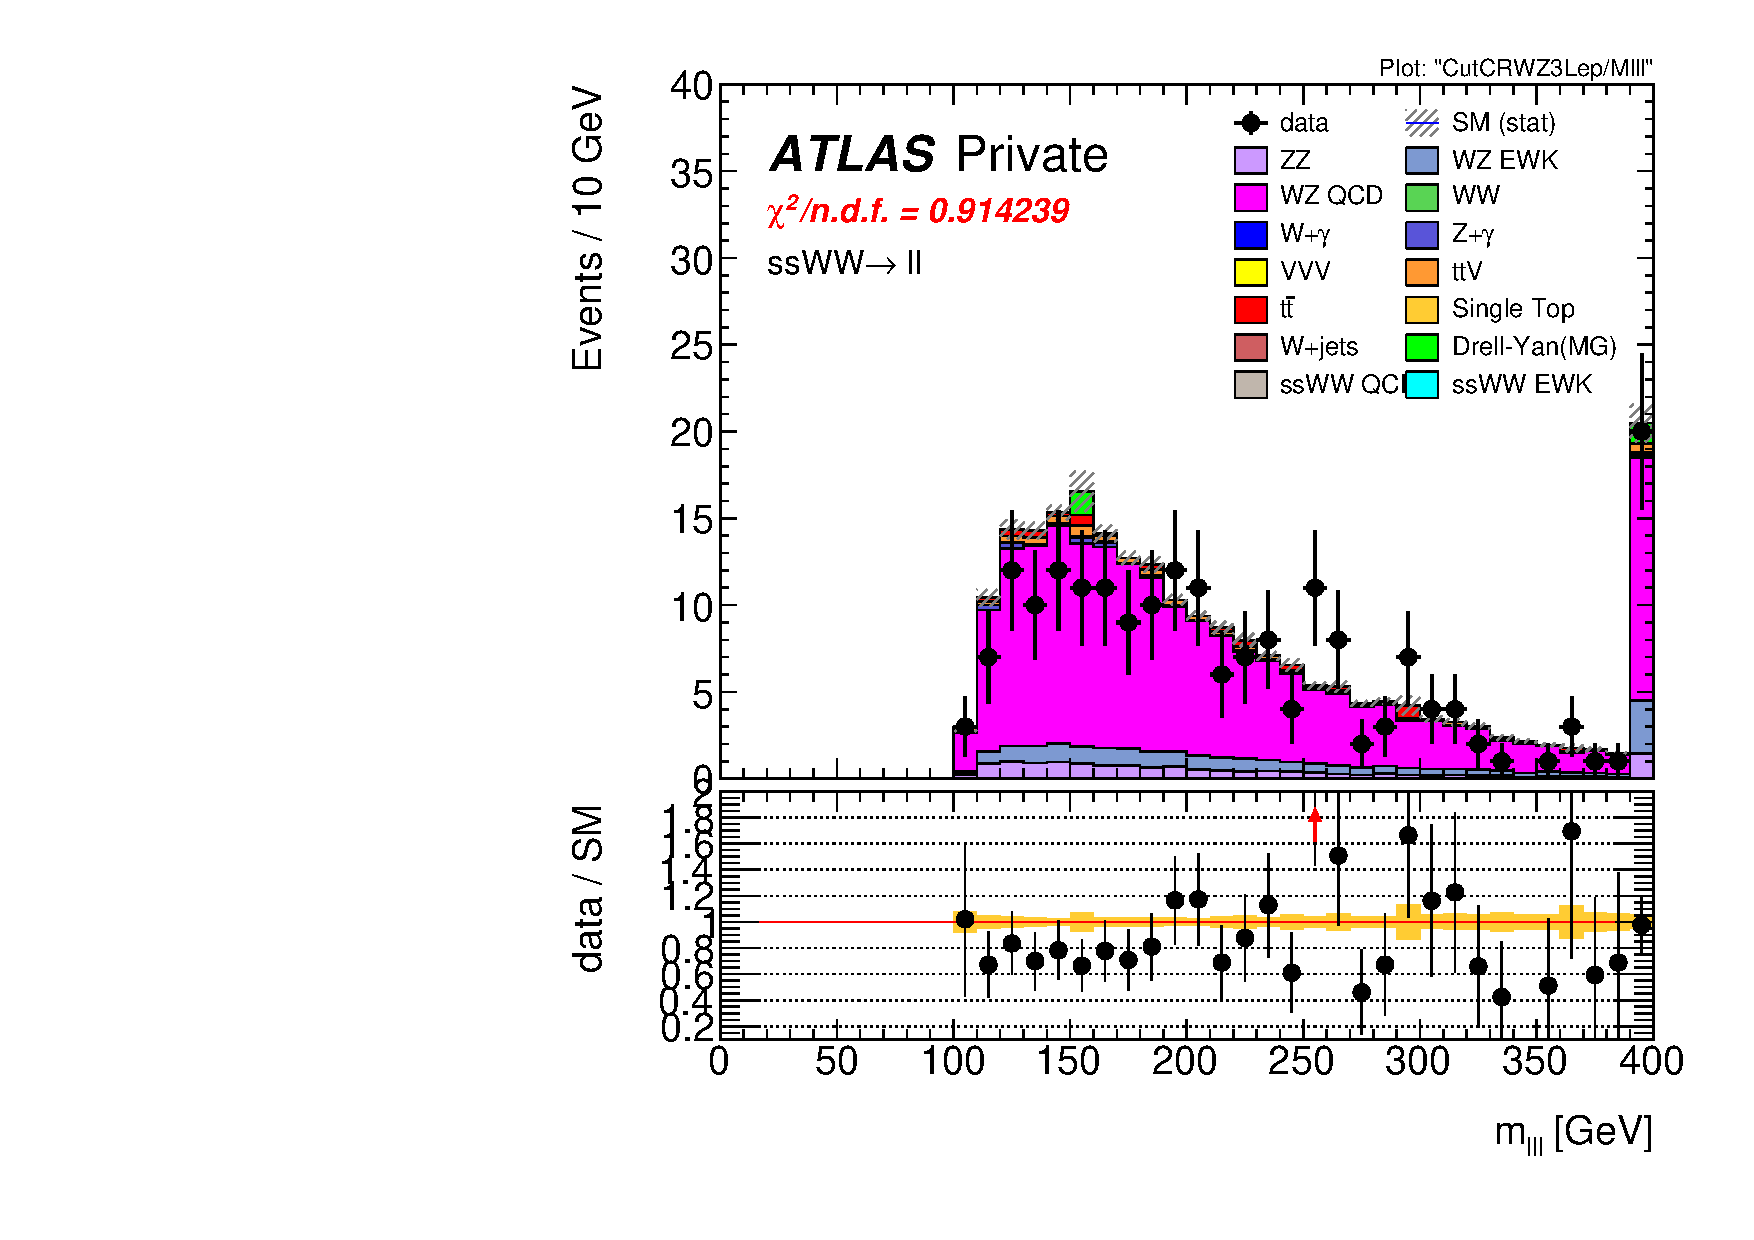
\includegraphics[width=.48\textwidth]{figs/ssww_13tev/backgrounds/wz/ll-CutCRWZ3Lep-Mlll-lin}
  \caption{Trilepton invariant mass $m_{lll}$ distribution in the $WZ$ control region before normalization.  All lepton channels are combined.}
  \label{fig:ssww13tev_wzcr_lep0}
\end{figure}

\subsection{Estimation of the $V\gamma$ background}\label{ssww13tev:wgamma}
Events from $V\gamma$ processes can pass selection if the photon converts into an $e^{+}e^{-}$ pair and one of the electrons passes the selection criteria.
The background is estimated from MC simulations which are then scaled by a normalization factor calculated from a control region enriched in $Z\rightarrow\mu\mu+\gamma$ events.
This control region selects two opposite-sign muons and an additional electron that is assumed to come from the photon conversion.
The full event selection is detailed in Table~\ref{tab:ssww13tev_vgamma_cr}.

\begin{table}[htbp]
  \centering
  \begin{tabular}{c}
    $V\gamma$ control region \\
    \hline\hline
    Exactly two muons with $\pt > 27\gev$ and $\pt > 20\gev$ \\
    Exactly one additional electron with $\pt > 15\gev$ \\
    Remove overlap between $Z$+jets and $Z\gamma$ \\
    Di-muon + photon invariant mass $75 < M_{\mu\mu\gamma} < 100\gev$ \\
    $\met < 30\gev$ \\
    \hline
  \end{tabular}
  \caption{Selection criteria for the $V\gamma$ control region.}
  \label{tab:ssww13tev_vgamma_cr}
\end{table}

The $Z\gamma$ MC samples available do not cover the full range of $\pt^\gamma$ and $\deltar(\gamma,l)$; thus, additional Drell-Yan samples ($Z$+jets) are used to fill out the phase space.
Overlap between the two samples are removed to avoid double counting.
Events with final state photons are checked at truth level\footnote{Truth particles are the particles produced directly by the MC generator before being passed through the full detector simulation, at which point they are considered \emph{reconstruction-level} (or \emph{reco-level}) particles.} to ensure that the photon did not originate from a hadronic decay.
Cuts on $\pt^\gamma > 10\gev$ and $\deltar(\gamma,l) > 0.1$ are then applied at generator level, and $Z\gamma$ events that fail this additional selection and $Z$+jets events that pass it are removed.

The normalization factor is calculated directly from the event yields in the $V\gamma$ control region rather than in the signal fit, as is done for the $WZ$ background.
The event yields are listed in Table~\ref{tab:ssww13tev_vgamma_numbers}, and the normalization factor is determined to be $1.77$.
No MC events from $Z\gamma$ processes survive the full event selection; thus, the scaling is only applied to the $W\gamma$ background in the signal region.
A systematic uncertainty of 44\% is assigned to the background based off of the uncertainties in the calculation of the normalization factor.

\begin{table}[htbp]
  \centering
  \begin{tabular}{l r}
    \multicolumn{2}{c}{Event yields in the $V\gamma$ control region} \\
    \hline\hline
    $Z\gamma$ & $24.6\pm 3.3$ \\
    $Z$+jets  &  $3.0\pm 1.5$ \\
    diboson + triboson & $6.7\pm 0.3$ \\
    top       &  $1.5\pm 0.5$ \\
    \hline
    Total prediction & $35.8\pm 3.7$ \\
    Data             & $57 \pm 7.6$ \\
    %\hline
    %Data - prediction & $21.2\pm 8.4$ \\
    \hline
  \end{tabular}
  \caption{Event yields in the $V\gamma$ control region.  The $V\gamma$ scale factor of 1.77 is calculated by scaling up the $Z\gamma$ and $Z$+jets backgrounds to account for the difference between the data and predicted total background.}
  \label{tab:ssww13tev_vgamma_numbers}
\end{table}

\subsection{Estimation of backgrounds from charge misidentification}\label{ssww13tev:charge_misid}
If an electron's charge is mis-reconstructed, it can lead to a real opposite-sign lepton pair passing the same-sign requirement in the event selection.
There are two primary reasons this can occur:
\begin{enumerate}
\item An electron emits a photon via bremsstrahlung which then converts into an electron-positron pair, and the conversion track with the wrong electric charge is matched to the original electron.
This is the dominant process leading to charge flip, and it is highly dependent on the electron $\eta$ due to the different amount of detector material the electron passes through.
\item The curvature of the electron's track is mis-measured, resulting in the wrong charge being assigned.
This process is dependent on the momentum of the electron, as its track becomes more straight as the momentum of the electron increases.
\end{enumerate}

In order to estimate this background, the rate at which an electron's charge is misidentified is calculated from $Z\rightarrow ee$ MC simulation.
It is known that the MC does not perfectly model the material effects leading to charge flip; as a result, scale factors are applied to the MC in order for it to to better reflect the real performance.
These scale factors are obtained from the ratio of charge mis-ID rates in data and uncorrected MC in~\cite{2018.ssww-13tev-atlas-support} following the method outlined in~\cite{2017.charge-flip-support}.
Once the scale factors are applied, the charge misidentification rate $\varepsilon$ can be extracted by comparing the electron's reconstructed charge with the charge of its truth particle:
\begin{equation}
  \varepsilon(\eta,\pt) = \frac{N_{\textrm{wrong\ charge}}}{N_{\textrm{prompt\ electrons}}}
\end{equation}
The charge mis-ID rate is calculated in bins of electron $|\eta|$ and $\pt$, and it varies from below $0.1\%$ in the central region of the detector up to $8\%$ in the forward regions for high $\pt$ (above $80\gev$) electrons.
A two-dimensional plot of $\varepsilon$ can be found in Figure~\ref{fig:charge_flip_rates}.

\begin{figure}
  \centering
  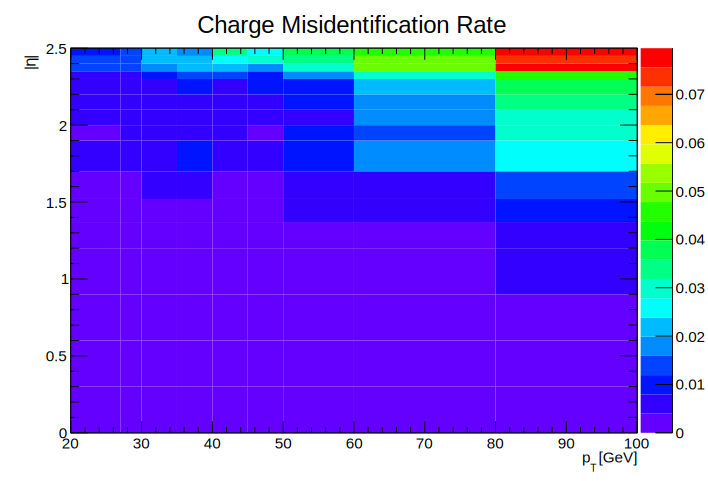
\includegraphics[width=.7\textwidth]{figs/ssww_13tev/backgrounds/charge_flip/charge_flip_2d}
  \caption{Charge misidentification rates for electrons as a function of $|\eta|$ and $\pt$.  Rates are calculated from $Z\rightarrow e^{+}e^{-}$ MC after applying sacle factors to approximate the charge mis-ID rates in data.}
  \label{fig:charge_flip_rates}
\end{figure}

%The size of the charge mis-ID background in a given region (signal or control region) is estimated from events that pass the region's default event selection but with an opposite-sign lepton pair.
Given the charge flip rate $\varepsilon(\eta,\pt)$, the rate at which an electron has its charge correctly reconstructed is $(1-\varepsilon)$.
Thus there are three possible combinations of charge identification, assuming a two-electron event:
\begin{enumerate}
\item Both electrons are reconstructed correctly: $(1-\varepsilon)^2$
\item Both electrons are mis-reconstructed: $\varepsilon^2$
\item Only one electron is mis-reconstructed: $2\varepsilon(1-\varepsilon)$
\end{enumerate}

In order to estimate the size of the background from charge misidentification, opposite-sign events are selected using the default event selection for a given signal or control region with the same-sign requirement inverted.
These events are then weighted by the probability for one of the electrons to be reconstructed with the wrong charge:
\begin{equation}
\omega = \frac{\varepsilon_1(1-\varepsilon_2)+\varepsilon_2(1-\varepsilon_1)}{(1-\varepsilon_1)(1-\varepsilon_2)+\varepsilon_1\varepsilon_2}
\label{ssww13tev:ch_flip_weight}
\end{equation}
%\begin{equation}
%\omega = \frac{\varepsilon_1(1-\varepsilon_2)+\varepsilon_2(1-\varepsilon_1)}{1-(\varepsilon_1+\varepsilon_2)+2\varepsilon_1\varepsilon_2}
%\label{ssww13tev:ch_flip_weight2}
%\end{equation}
where the subscripts 1 and 2 refer to the leading and subleading electrons, respectively, and $\varepsilon_i$ is a function of the $\eta$ and $\pt$ of the $i^{\textrm{th}}$ electron.
In the case of an event with one electron and one muon ($\varepsilon_\mu = 0$), Equation~\ref{ssww13tev:ch_flip_weight} simplifies:
\begin{equation}
\omega = \frac{\varepsilon}{1-\varepsilon}
\end{equation}
This method assumes that there is little contamination from fake electrons in the opposite-sign sample, and this has been verified with MC simulation.

Additionally, charge-flipped electrons tend to be reconstructed with lower energy when compared to electrons with the correct charge.
This is due to energy loss from the material interactions that can cause the charge to be misidentified in the first place.
A correction factor is calculated from MC simulations, comparing the $\pt$ of the truth electron to its reconstructed counterpart:
\begin{equation}
\alpha = \frac{\Big(\frac{\pt^{\textrm{reco}}}{\pt^{\textrm{truth}}}-1\Big)_{\textrm{correct charge}}}{\Big(\frac{\pt^{\textrm{reco}}}{\pt^{\textrm{truth}}}-1\Big)_{\textrm{wrong charge}}}
\label{ssww13tev:ch_flip_alpha}
\end{equation}
The correction is then applied to the $\pt$ of the charge-flipped electron via
\begin{equation}
\pt = \pt^0/(1+\alpha)+dE
\label{ssww13tev:ch_flip_energy_corr}
\end{equation}
where $\pt^0$ is the uncorrected $\pt$ of the electron and $dE$ is a gaussian smearing factor centered at zero with a width related to the energy resolution.
Since which electron is mis-reconstructed is never determined in this method, in the case of a two-electron event, the energy correction is applied randomly to one of the two electrons based on the probabilities for them to be charge-flipped.
This also determines the overall sign of the event; the charge of the electron that does not recieve the correction is taken to be the charge for both.

Systematic uncertainties on the charge mis-ID rates are calculated by generating two additional sets of rates with the uncertainties on the scale factors varied up and down.
The size of the estimated charge flip background without the energy correction applied is also taken as a systematic uncertainty.
These systematic uncertainties are estimated to be approximately $\pm 15\%$.

\subsubsection{Validation of the charge misidentification estimate}\label{ssww13tev:ssincl_vr}
%The performance of the charge misidentification estimation is tested in $e^{\pm}e^{\pm}$ events with a di-electron invariant mass that lies within $15\gev$ of the $Z$ boson mass.
%Disagreements between data and background at high $\pt$ and $\eta$ have been found to be due to backgrounds from misidentified leptons, which are not included due to unreliable modeling in this particular region.

The performance of the charge misidentification estimation is tested in the same-sign inclusive validation region (VR), defined in Table~\ref{tab:ssww13tev_ssincl_vr_def}.
For $ee$ events, the mass of the dilepton pair is required to lie within $15\gev$ of the $Z$ boson mass to increase the purity of the charge flip background.
$t\bar{t}$ production, which can contribute to both the charge mis-ID and fake lepton backgrounds, is suppressed by the $b$-jet veto.
The di-electron invariant mass is shown in Figure~\ref{fig:ssww13tev_ssincl_mll}, and distributions of the leading and subleading electron $\pt$ in the $ee$-channel are shown in Figure~\ref{fig:ssww13tev_ssincl_ptlep} with the $Z$ mass cut inverted.
Agreement between data and prediction is seen within the total statistical and systematic uncertainties in the VR.

\begin{table}[htbp]
  \centering
  \begin{tabular}{c}
    Same-sign inclusive VR \\
    \hline\hline
    Exactly 2 same-sign signal leptons\\
    $\pt > 27\gev$ for both leptons \\
    $m_{ll} > 20\gev$\\
    $|m_{ee} - m_Z| > 15\gev$ ($\ee$-channel only) \\
    $N_{b\textrm{-jet}} = 0$\\
    \hline
  \end{tabular}
  \caption{Selection criteria for the same-sign inclusive validation region.}
  \label{tab:ssww13tev_ssincl_vr_def}
\end{table}

\begin{figure}
  \centering
  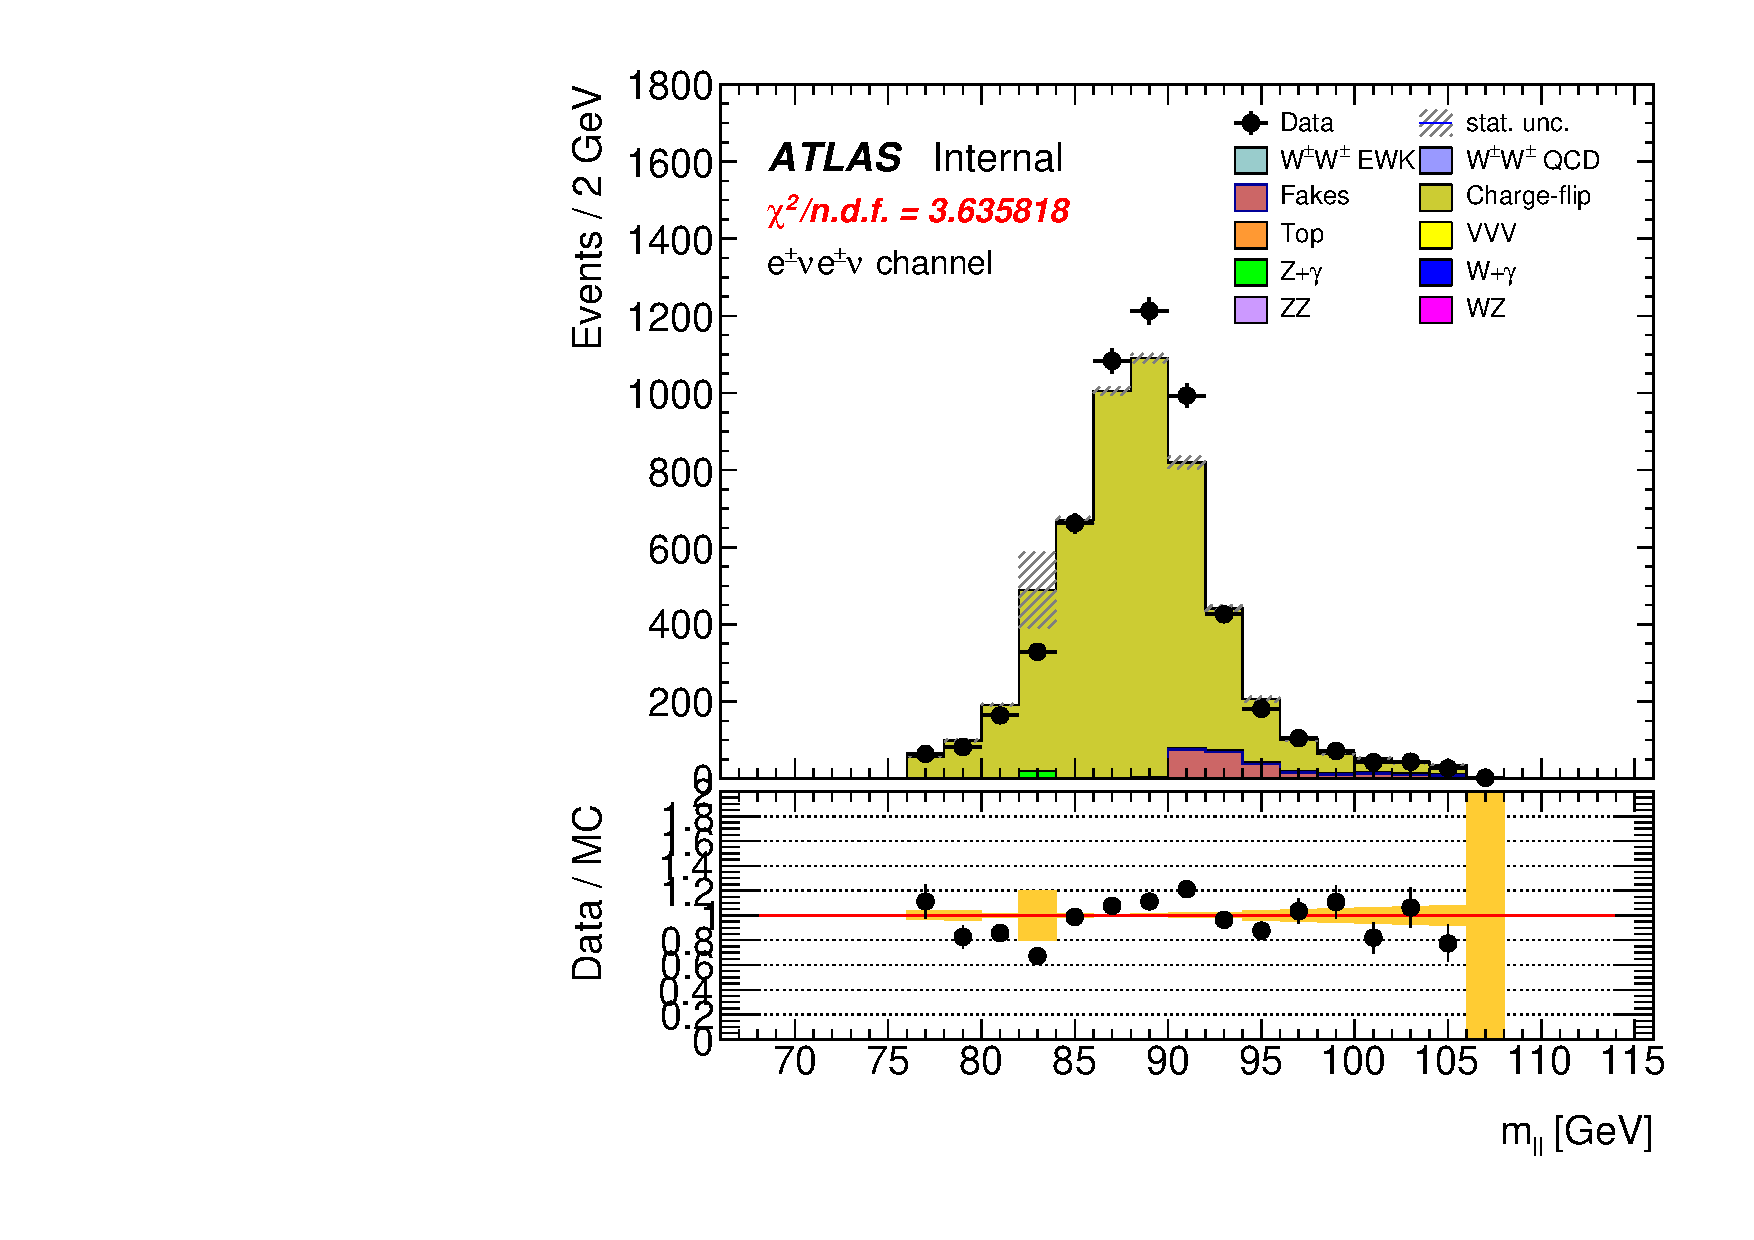
\includegraphics[width=.48\textwidth]{figs/ssww_13tev/backgrounds/charge_flip/ee-CutCRInclusiveSSZ-Mll_Zpeak-lin}
  \caption{Dilepton invariant mass distribution $m_{ll}$ for the $ee$ channel in the same-sign inclusive VR.}
  \label{fig:ssww13tev_ssincl_mll}
\end{figure}

\begin{figure}
  \centering
  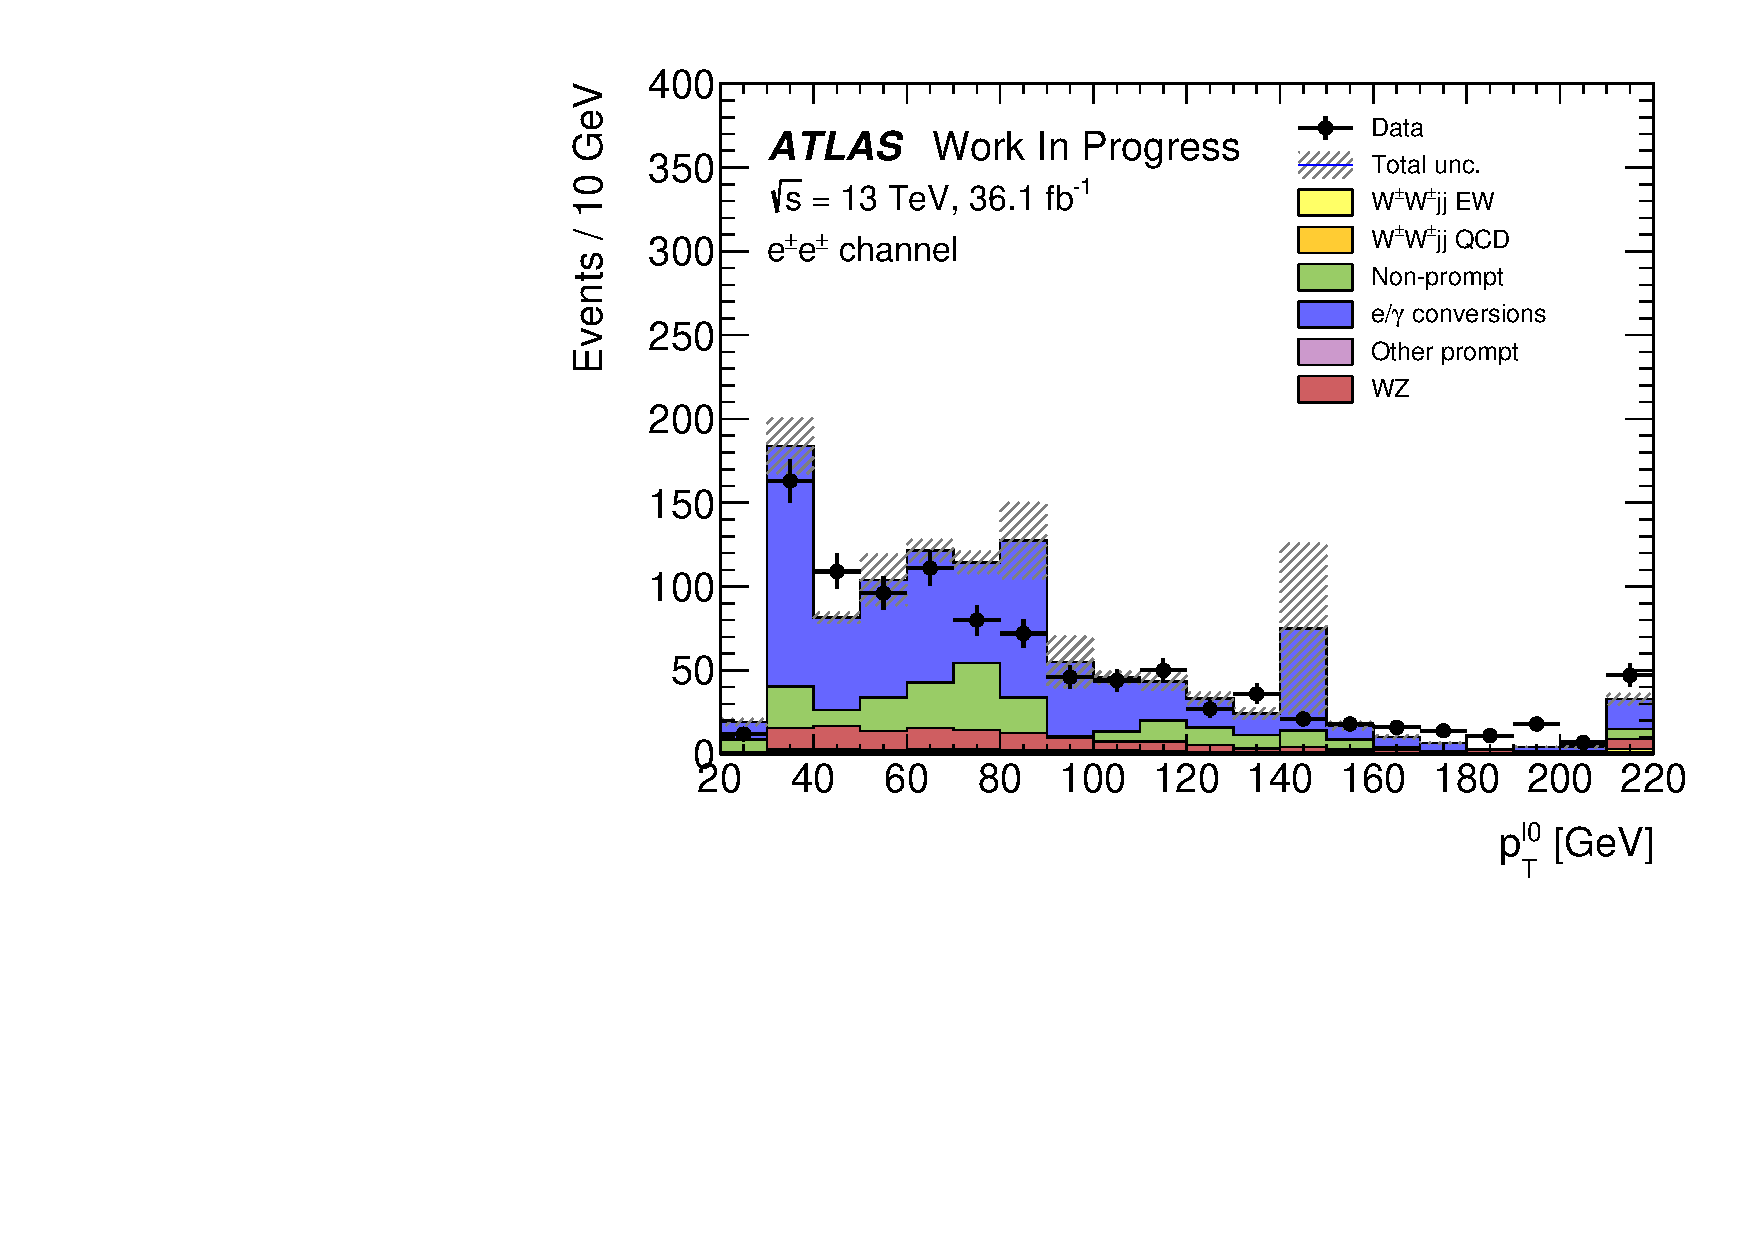
\includegraphics[width=.48\textwidth]{figs/ssww_13tev/backgrounds/charge_flip/ee-CutCRInclusiveSSZVeto-l0_pt-lin.pdf}
  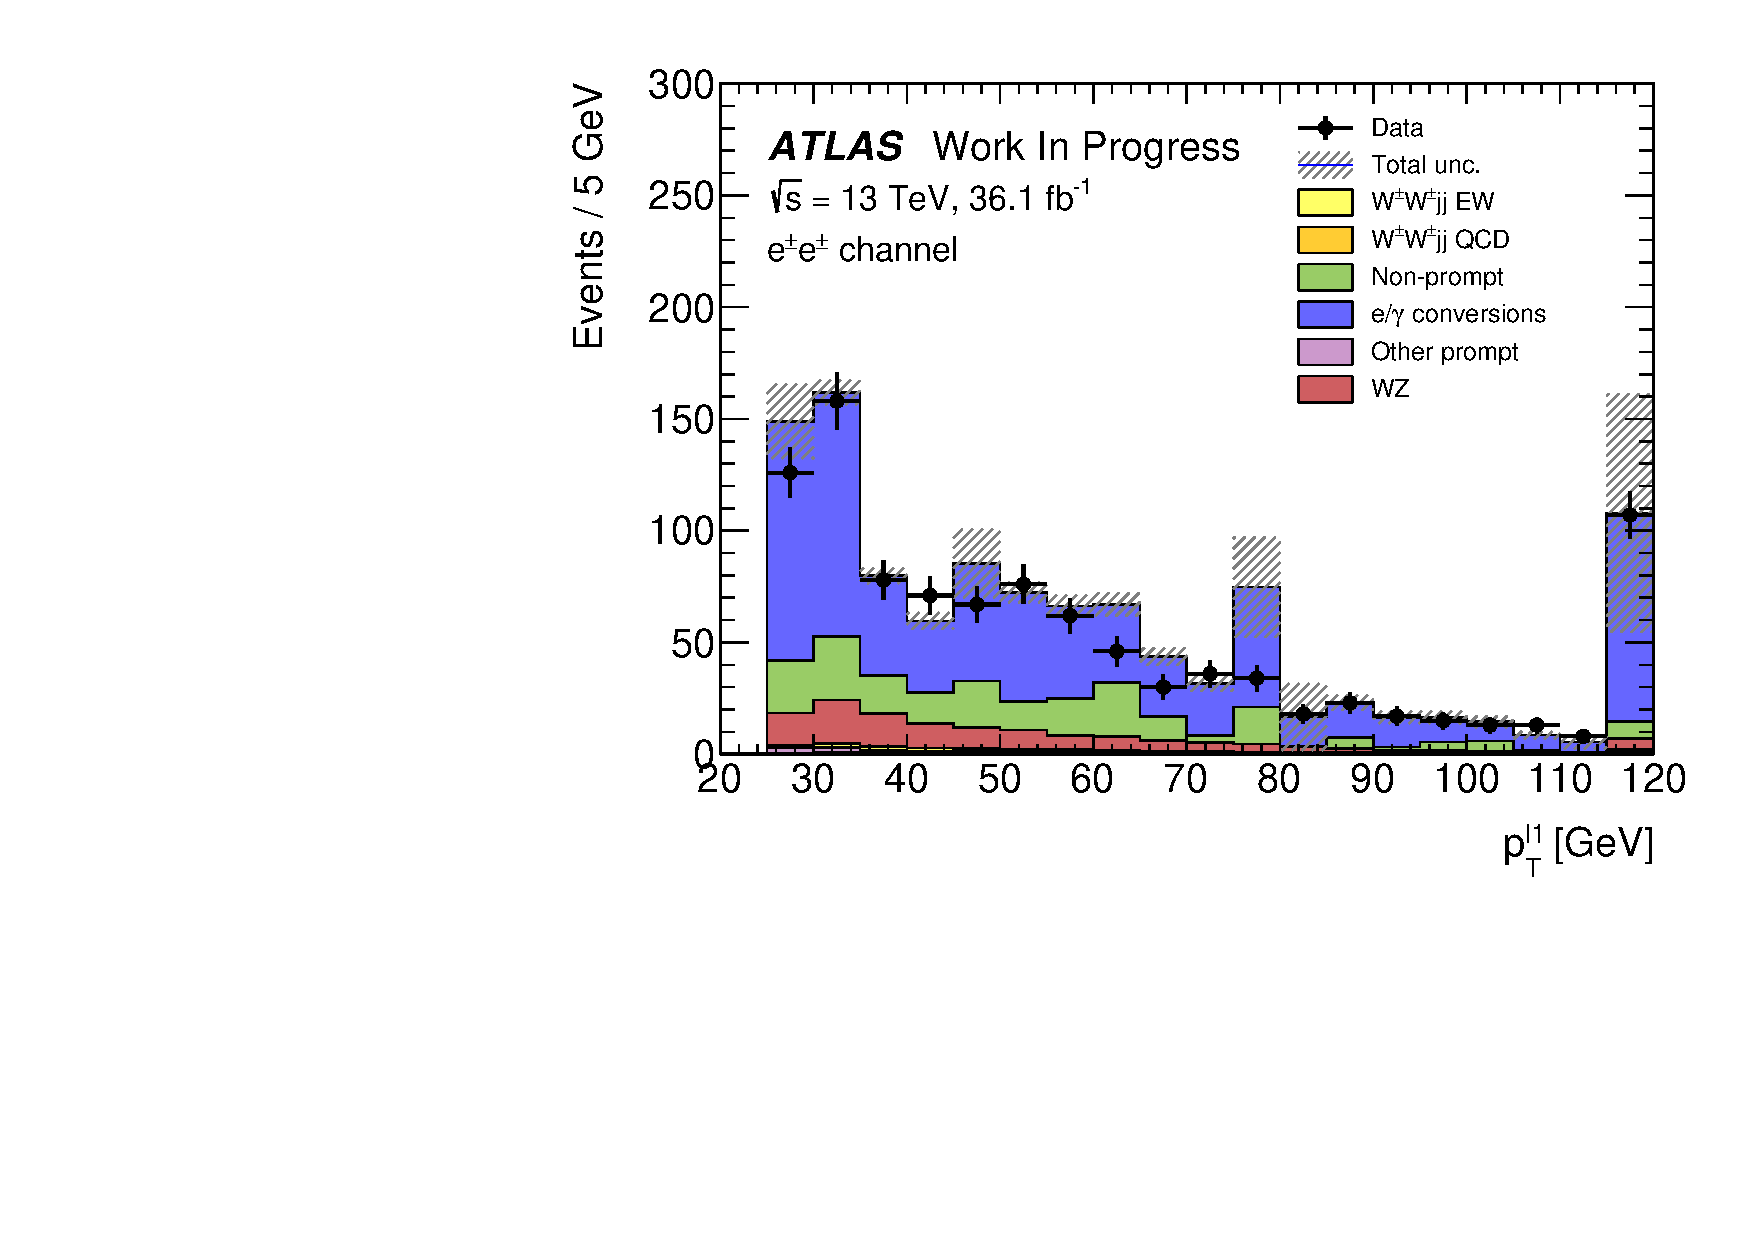
\includegraphics[width=.48\textwidth]{figs/ssww_13tev/backgrounds/charge_flip/ee-CutCRInclusiveSSZVeto-l1_pt-lin.pdf}
  \caption{$\pt$ distributions for the leading (left) and subleading (right) electron for the $ee$ channel in the same-sign inclusive VR.  In these plots, the cut requiring $m_{ee}$ to fall within the $Z$ mass window has been inverted in order to test the modelling away from the $Z$ peak.}
  \label{fig:ssww13tev_ssincl_ptlep}
\end{figure}

\subsection{Estimation of non-prompt backgrounds with the fake-factor method}\label{ssww13tev:fake_factor}
fake factor method


\subsection{Reduction of $WZ$ background using custom overlap removal}\label{ssww13tev:custom_or}
The dominant source of prompt background in this analysis comes from $WZ$ events where both bosons decay leptonically.
Traditionally, the background is dealt with by imposing a veto on any event with a third lepton passing some loose identification criteria (the so-called \emph{trilepton veto}).
In the case of this analysis, if one or more leptons (in addition to the two signal leptons) passed the preselection criteria, the event would be rejected.
However, $WZ$ events can still enter the signal region if one of the leptons fails the veto selection or falls outside of the detector's acceptance.

In order to understand the sources of $WZ$ events that are not removed by the trilepton veto, a study was performed on truth-level leptons\footnote{Truth particles are the particles produced directly by the MC generator before being passed through the full detector simulation, at which point they are considered \emph{reconstruction-level} (or \emph{reco-level}) particles.} on \ssww and $WZ$ MC samples.
Events with three truth leptons were selected, and each was matched to its reconstruction-level partner by finding the closest $\deltar(\textrm{truth},\textrm{reco})$ and $\Delta p_{\textrm{T},\textrm{truth},\textrm{reco}}$ match.
For events surviving the trilepton veto, the two signal leptons were removed, and the remaining leptons represent real leptons that failed to be selected for the veto.
Between 40-50\% of these leptons fell outside of the eta acceptance of the analysis (see Figure~\ref{fig:ssww13tev_wzveto_truthlepeta}) and were unrecoverable.
The second largest source of leptons failing the preselection was the overlap removal (OR). \TODO{Make sure to define overlap removal in the event selection section!}
The standard OF procedure appeared to be too aggressive in removing leptons in favor of jets, causing many three lepton events to ``lose'' their third lepton and pass the trilepton veto.

\begin{figure}[htbp]
  \centering
  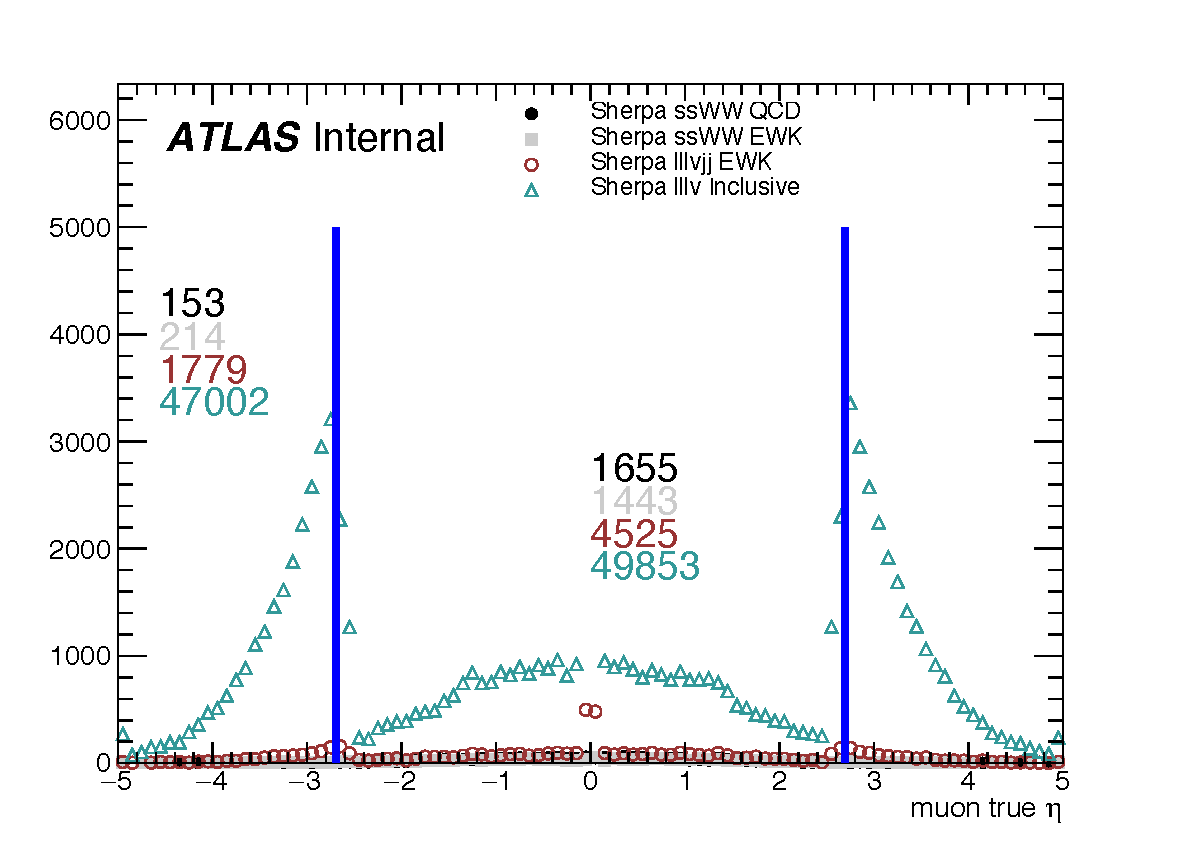
\includegraphics[width=.48\textwidth]{figs/ssww_13tev/custom_or/ExtraMuonEta_counted}
  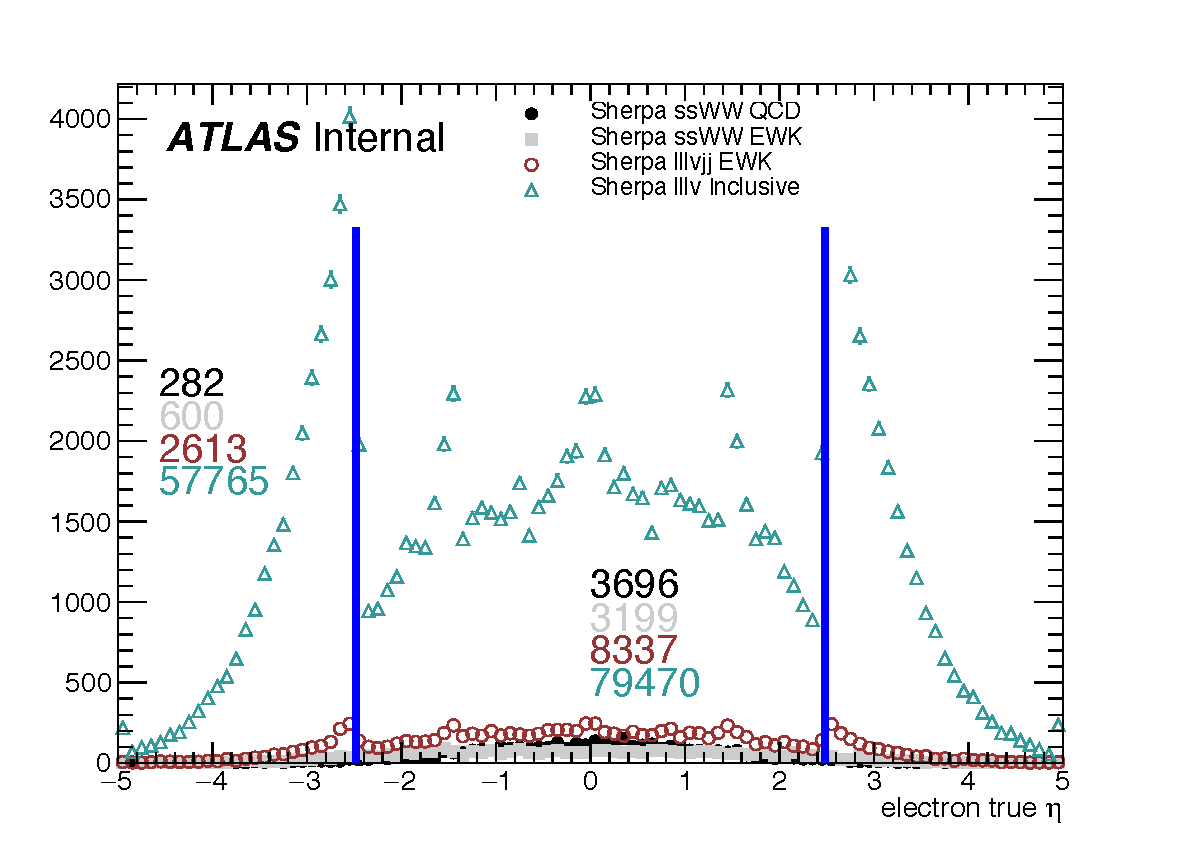
\includegraphics[width=.48\textwidth]{figs/ssww_13tev/custom_or/ExtraElecEta_counted}
  \caption{Pseudorapidity ($\eta$) distributions of truth muons (top) and electrons (bottom) for Sherpa \ssww and $WZ$ MC samples.  The blue vertical lines represent the allowed $\eta$ range for each lepton flavor.  The numbers correspond to the number of raw MC events that fall within and outside of the allowed $\eta$ range for each MC sample.}
  \label{fig:ssww13tev_wzveto_truthlepeta}
\end{figure}

Two quantities were chosen to construct a ``custom'' OR that would 

\begin{figure}[htbp]
  \centering
  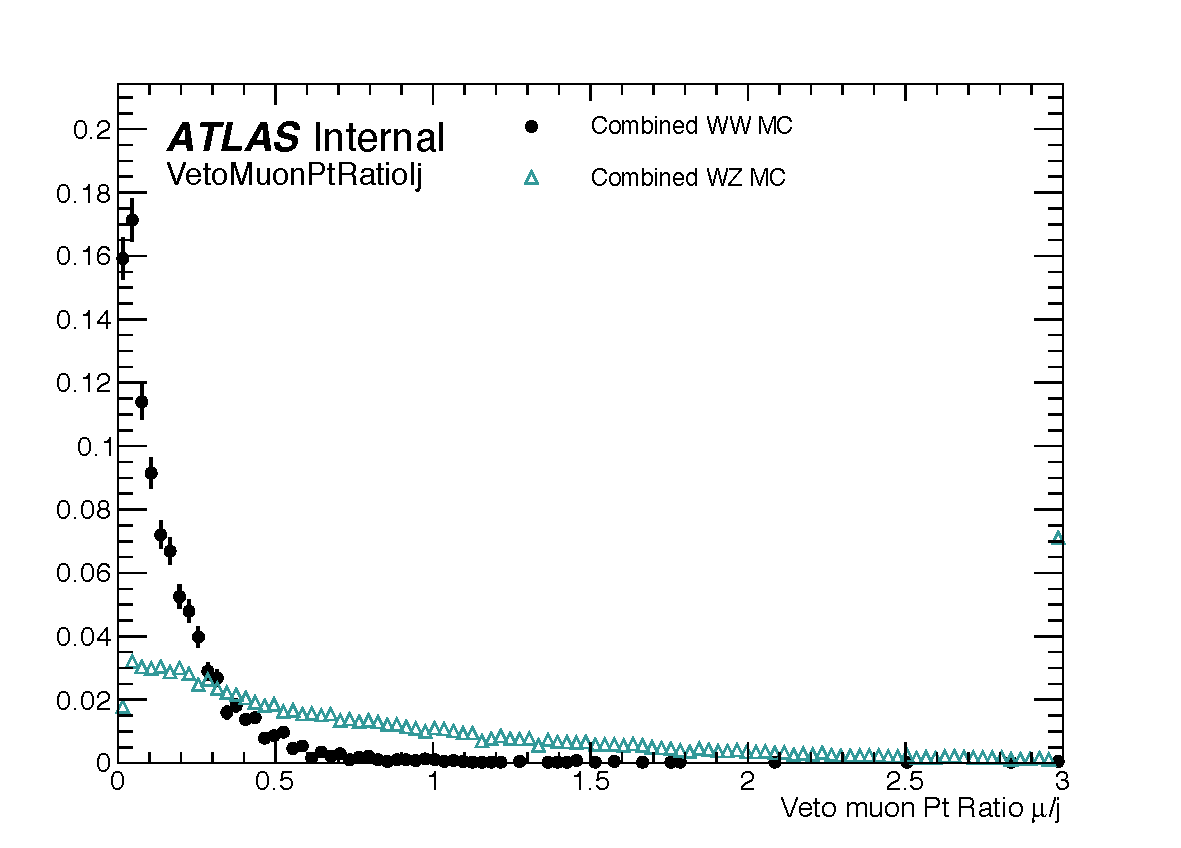
\includegraphics[width=.48\textwidth]{figs/ssww_13tev/custom_or/VetoMuonPtRatiolj}
  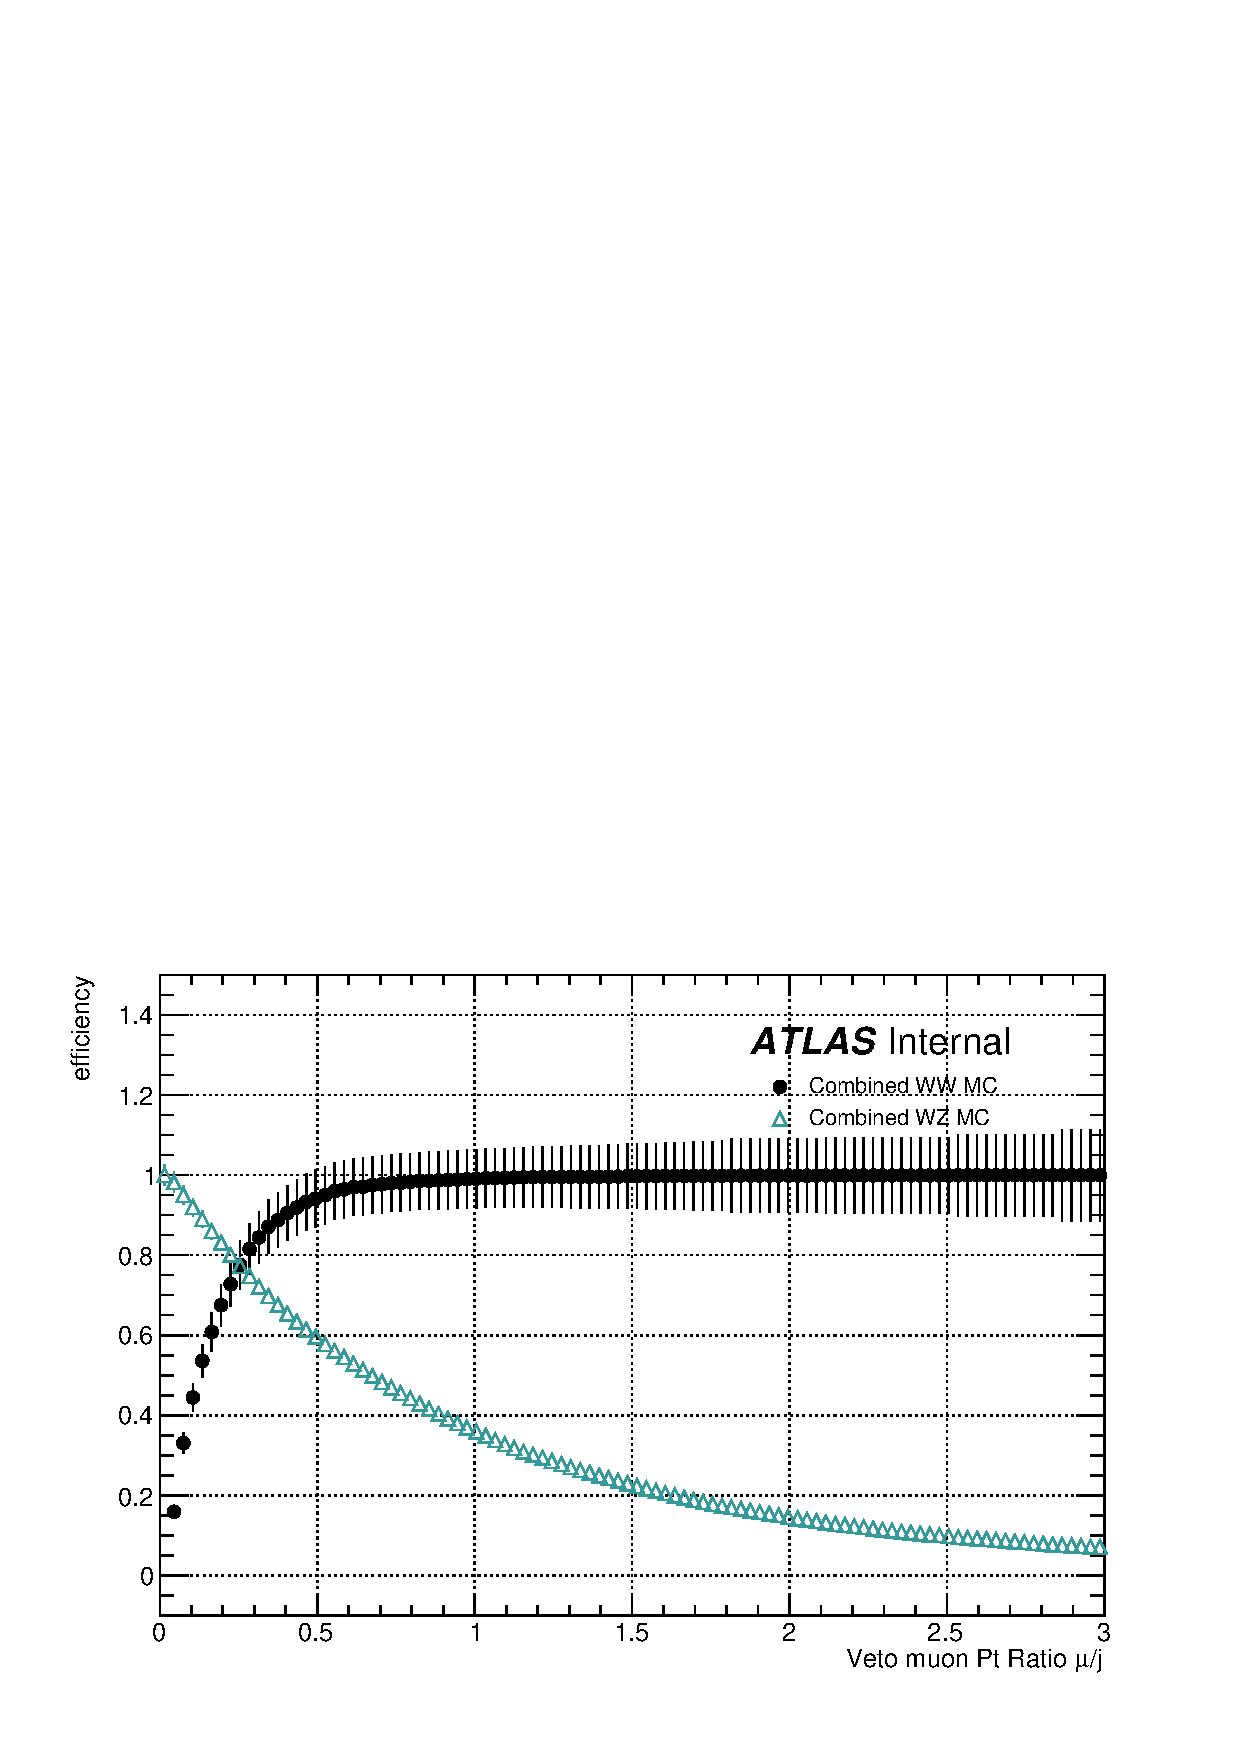
\includegraphics[width=.48\textwidth]{figs/ssww_13tev/custom_or/ROC_VetoMuonPtRatiolj}\\
  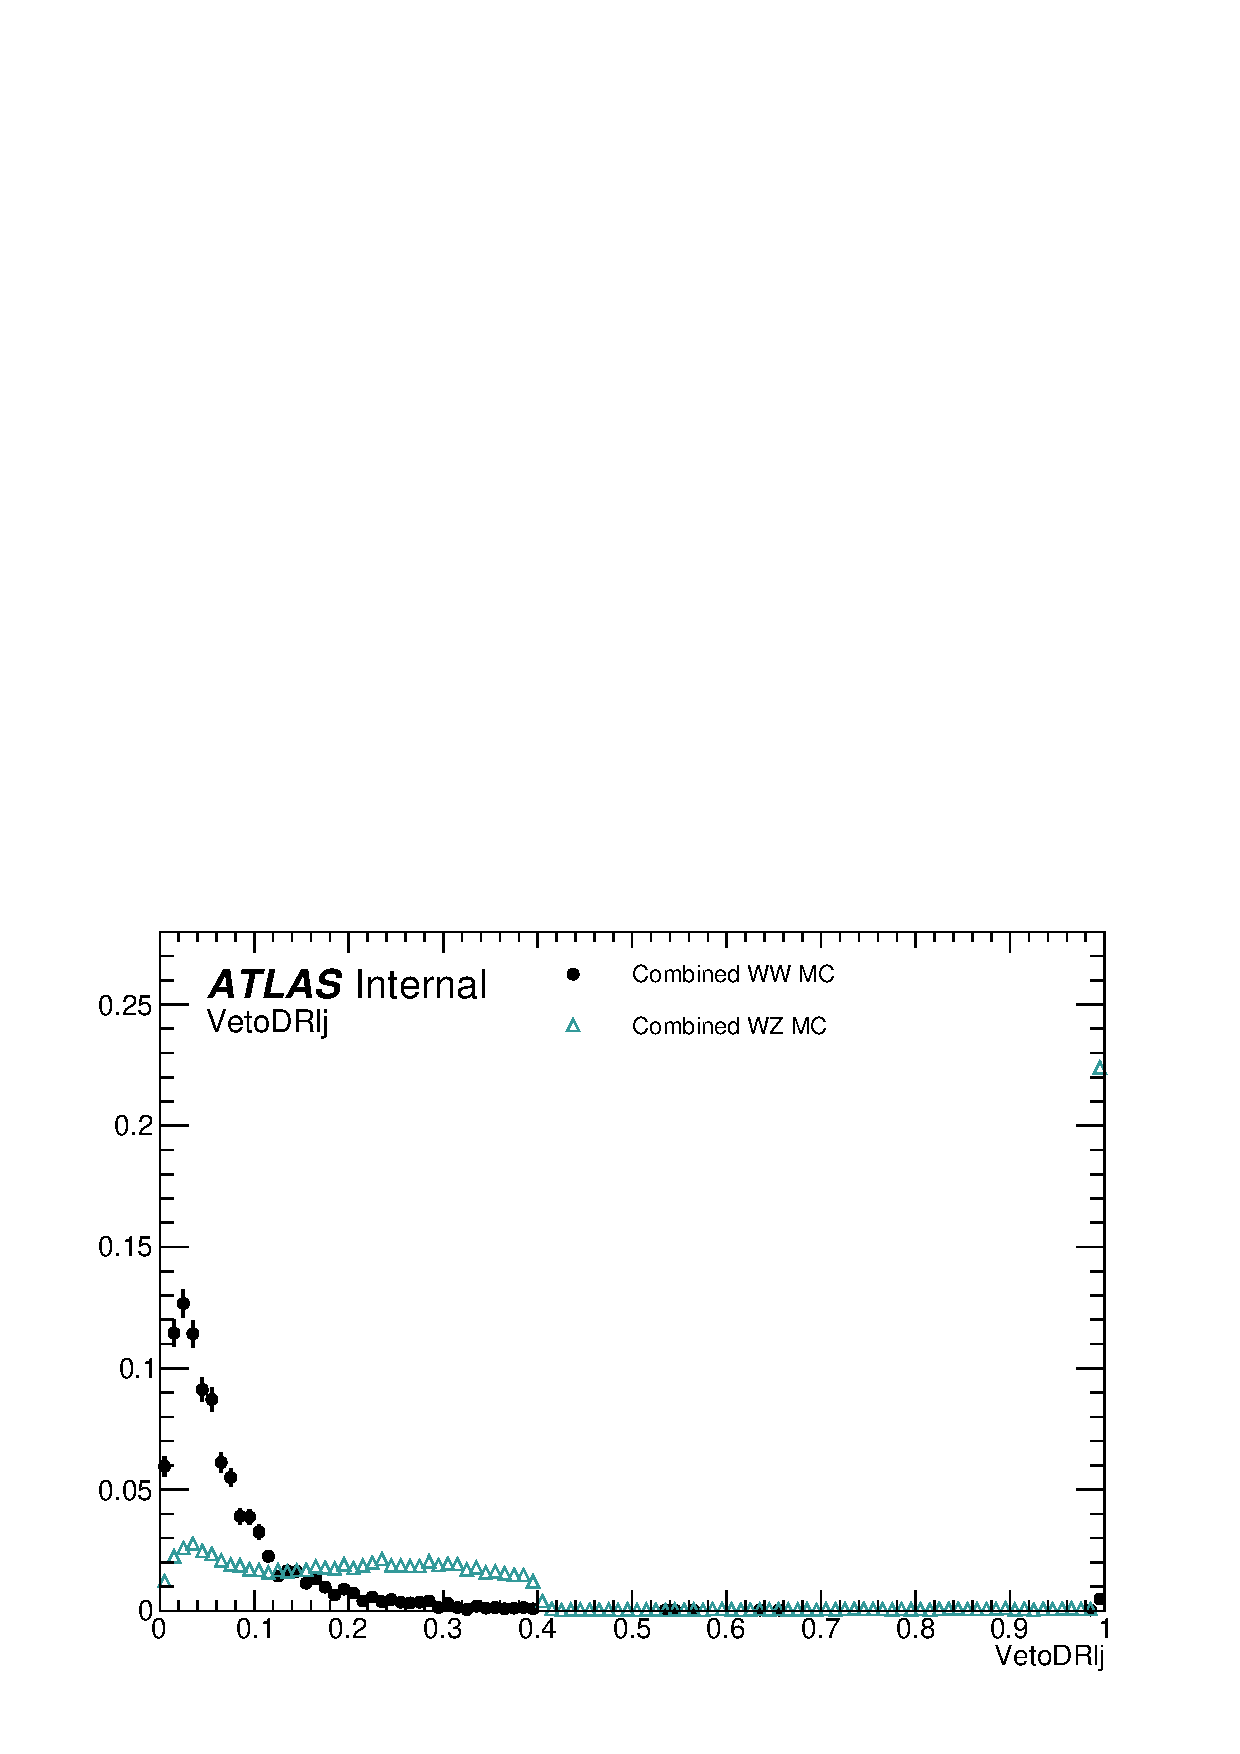
\includegraphics[width=.48\textwidth]{figs/ssww_13tev/custom_or/veto_muon_VetoDRlj}
  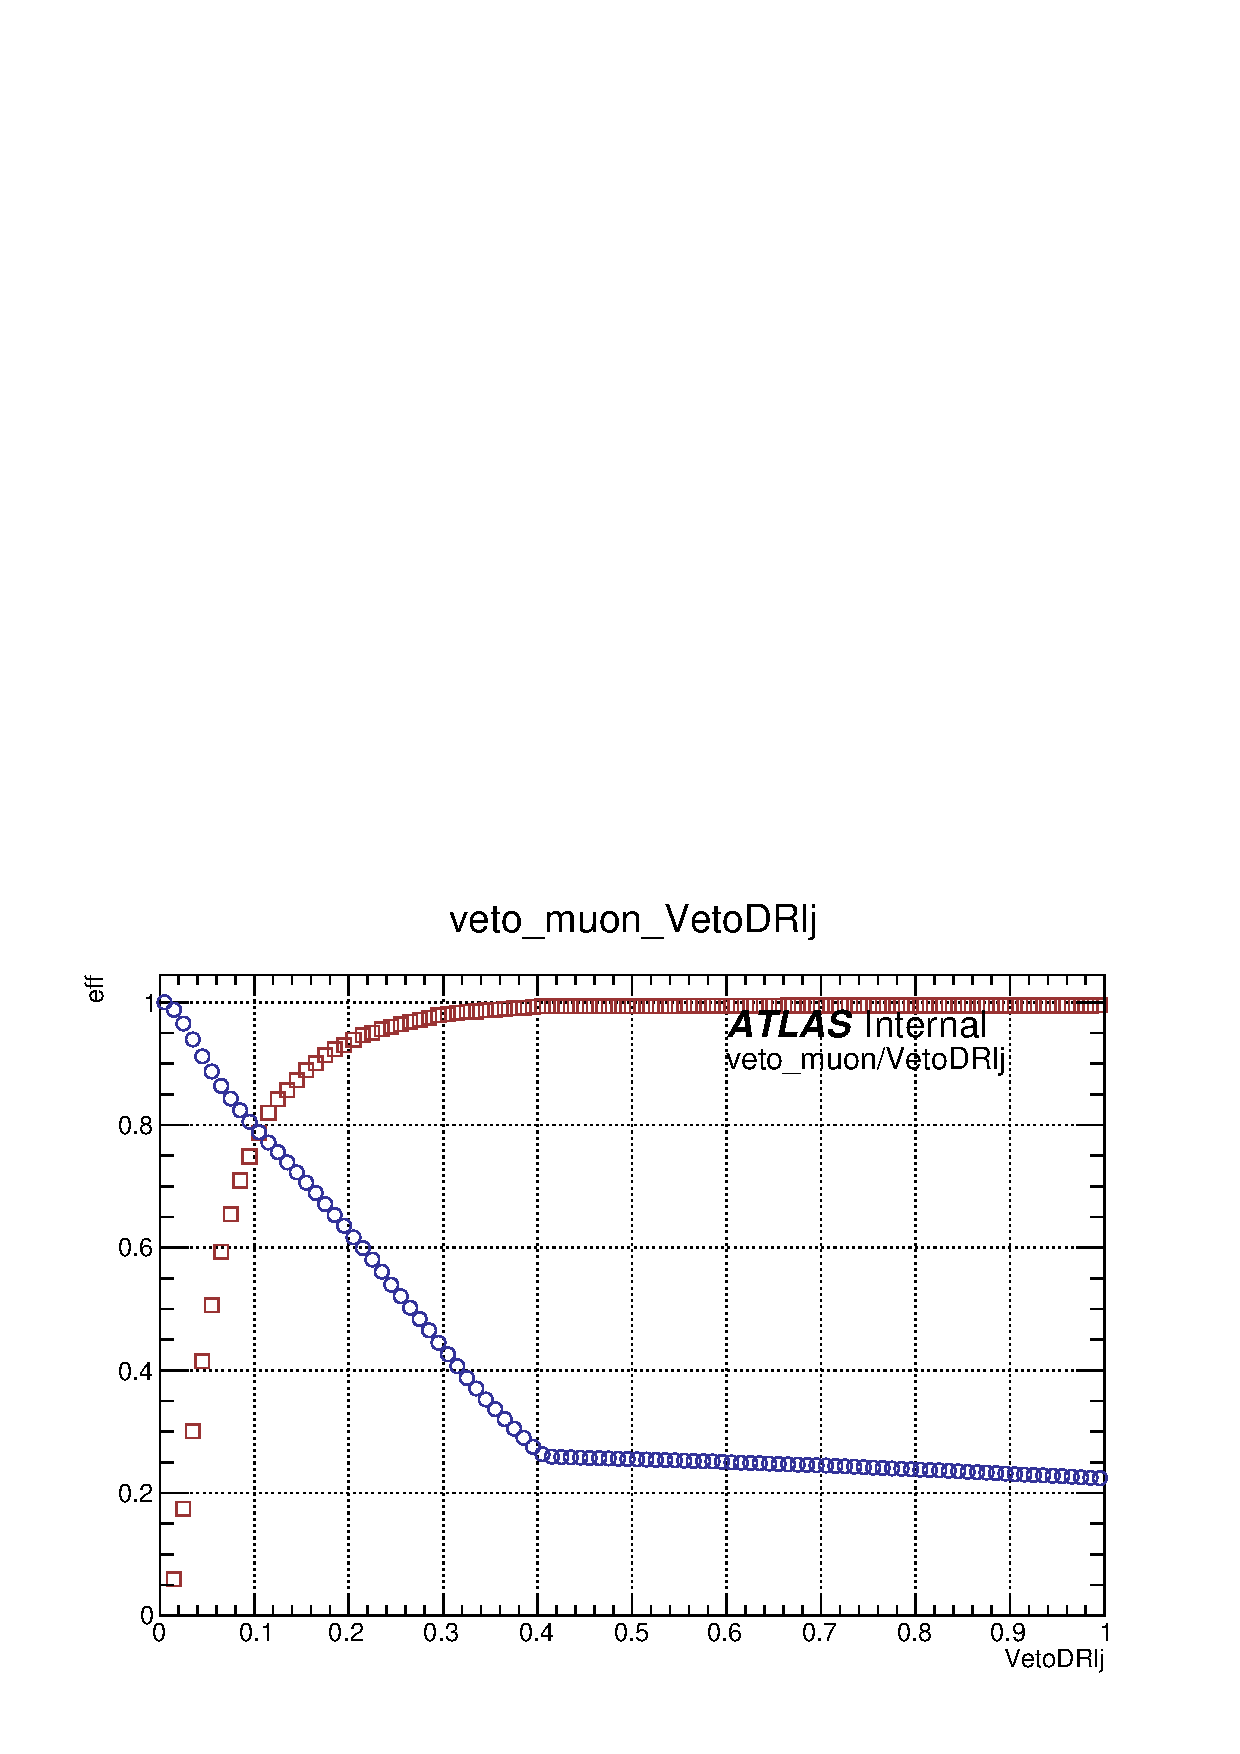
\includegraphics[width=.48\textwidth]{figs/ssww_13tev/custom_or/ROC_veto_muon_VetoDRlj}\\
  \caption{Stuff}
  \label{fig:ssww13tev_customor_muon}
\end{figure}

\begin{figure}[htbp]
  \centering
  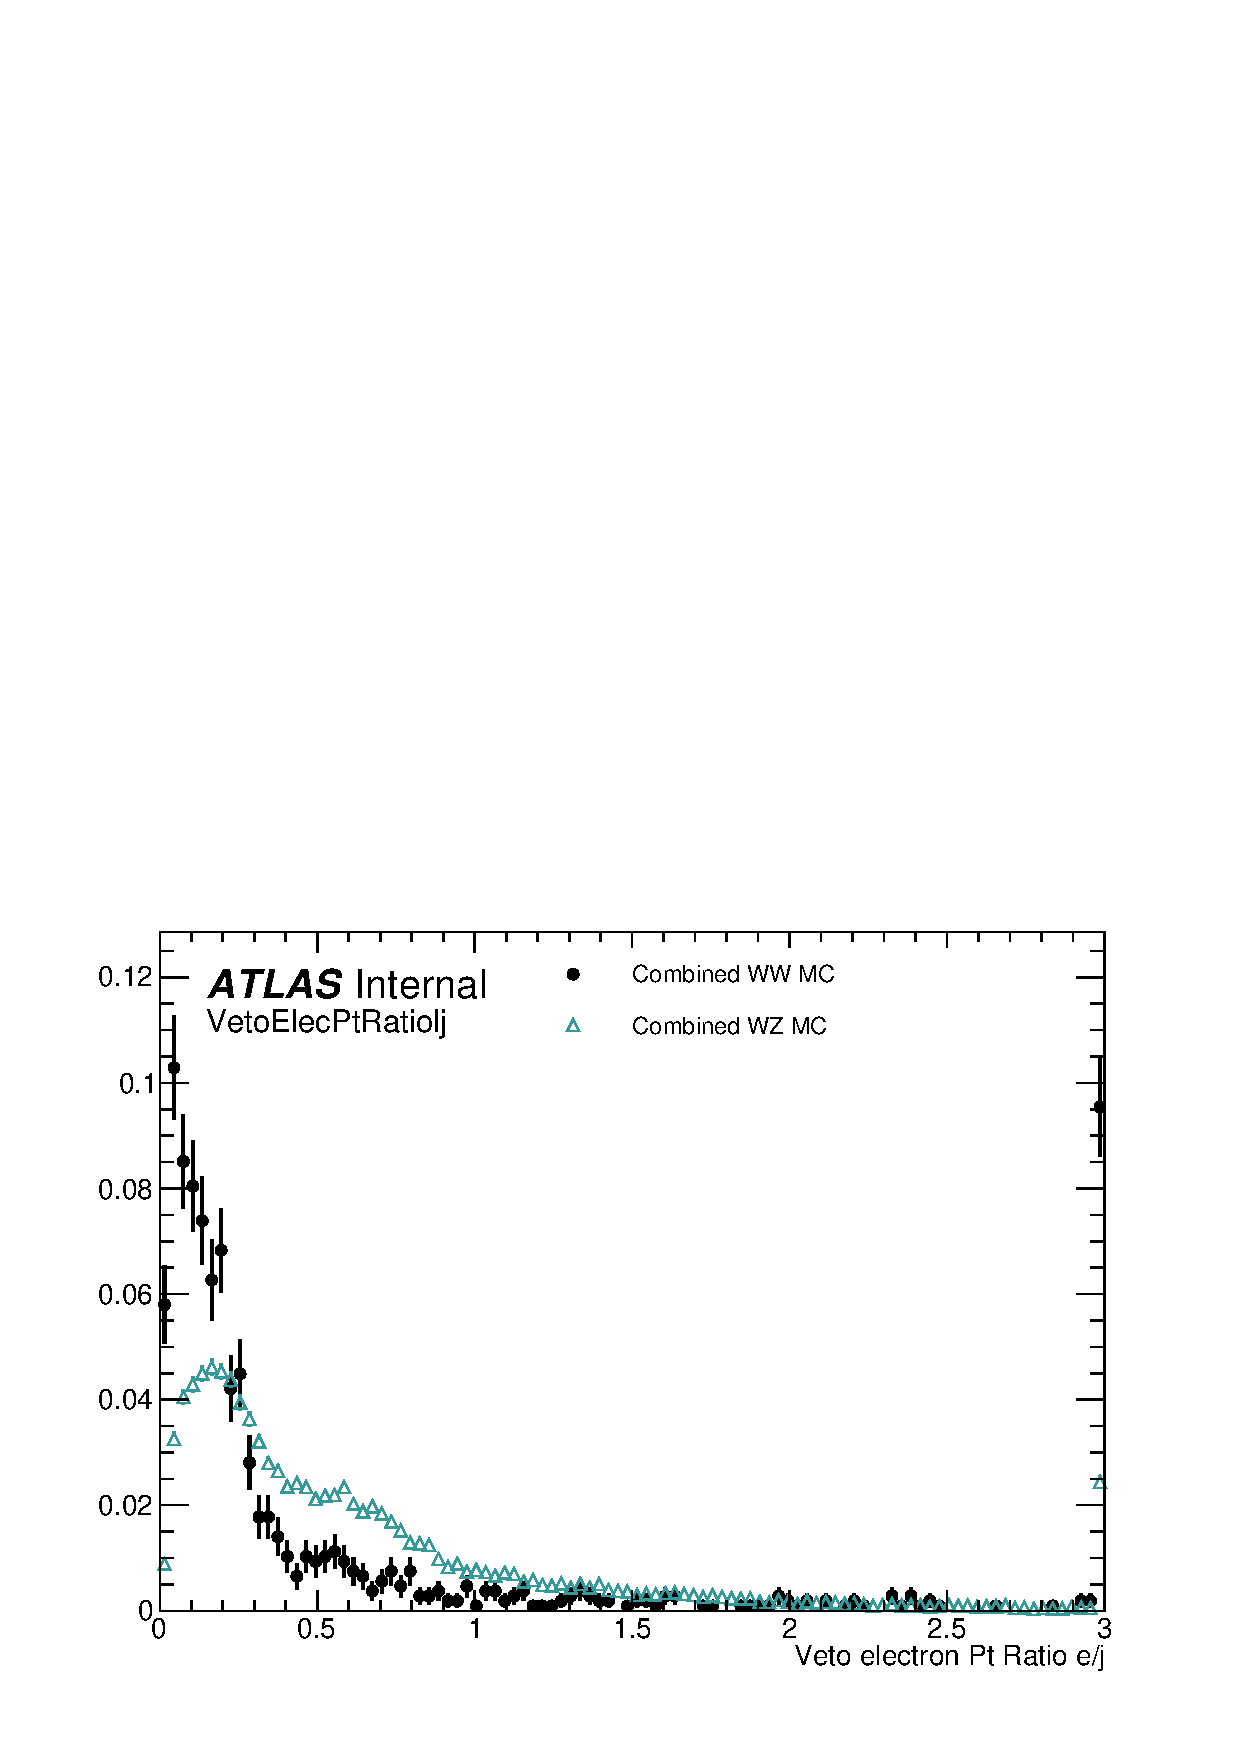
\includegraphics[width=.48\textwidth]{figs/ssww_13tev/custom_or/VetoElecPtRatiolj}
  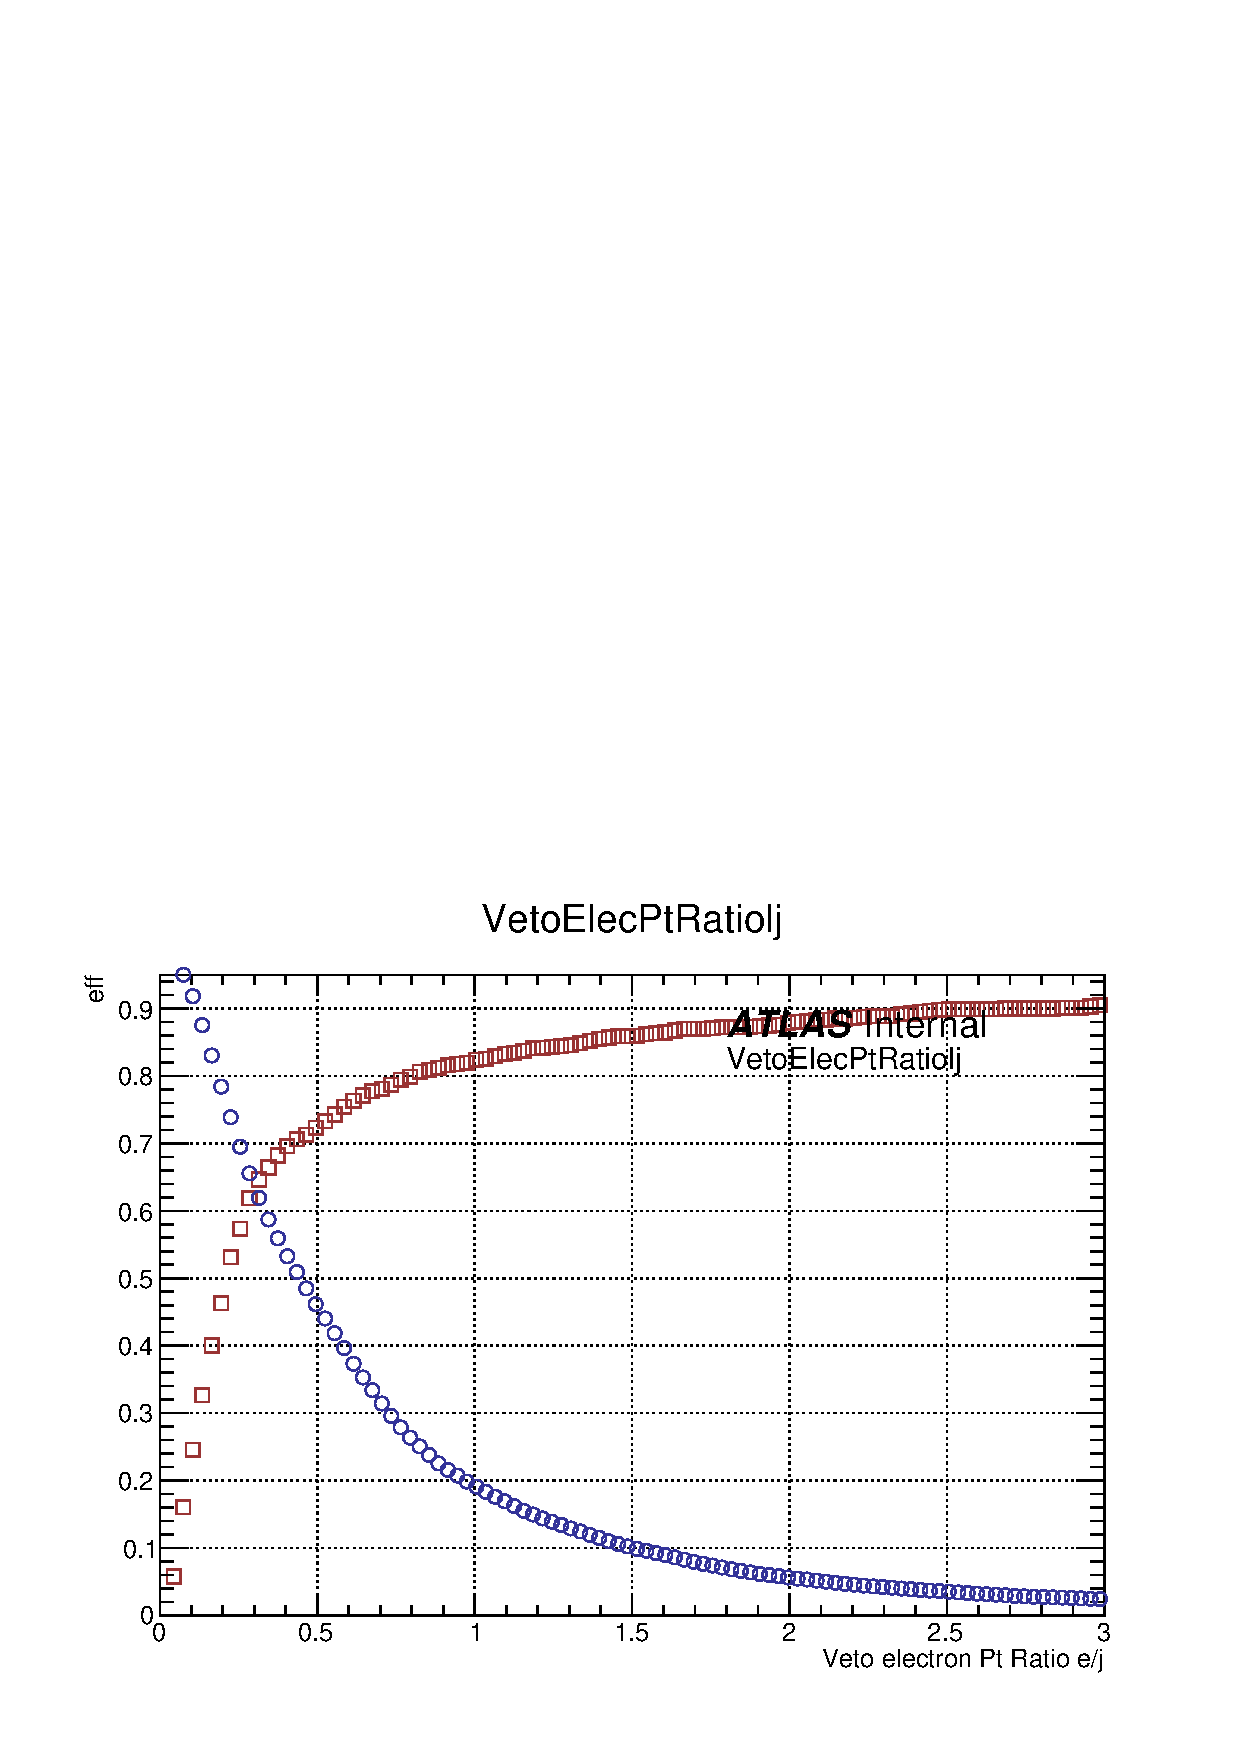
\includegraphics[width=.48\textwidth]{figs/ssww_13tev/custom_or/ROC_VetoElecPtRatiolj}
  \caption{Stuff}
  \label{fig:ssww13tev_customor_elec}
\end{figure}

\begin{figure}[htbp]
  \centering
  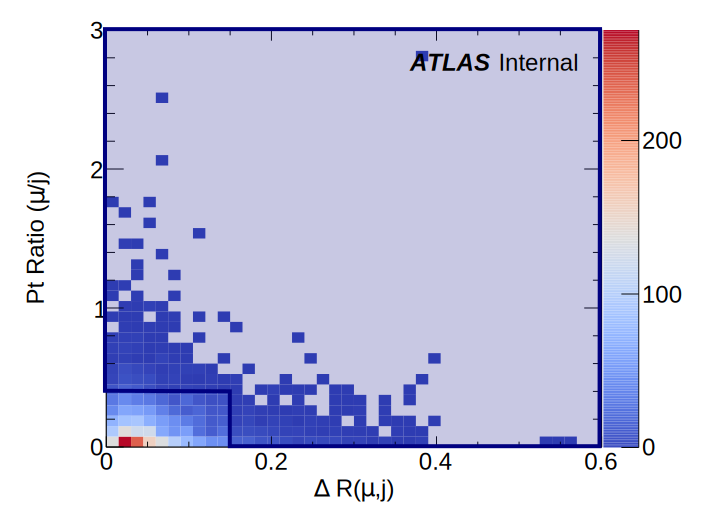
\includegraphics[width=.48\textwidth]{figs/ssww_13tev/custom_or/sig_Muon_DR_PtRatio_edited}
  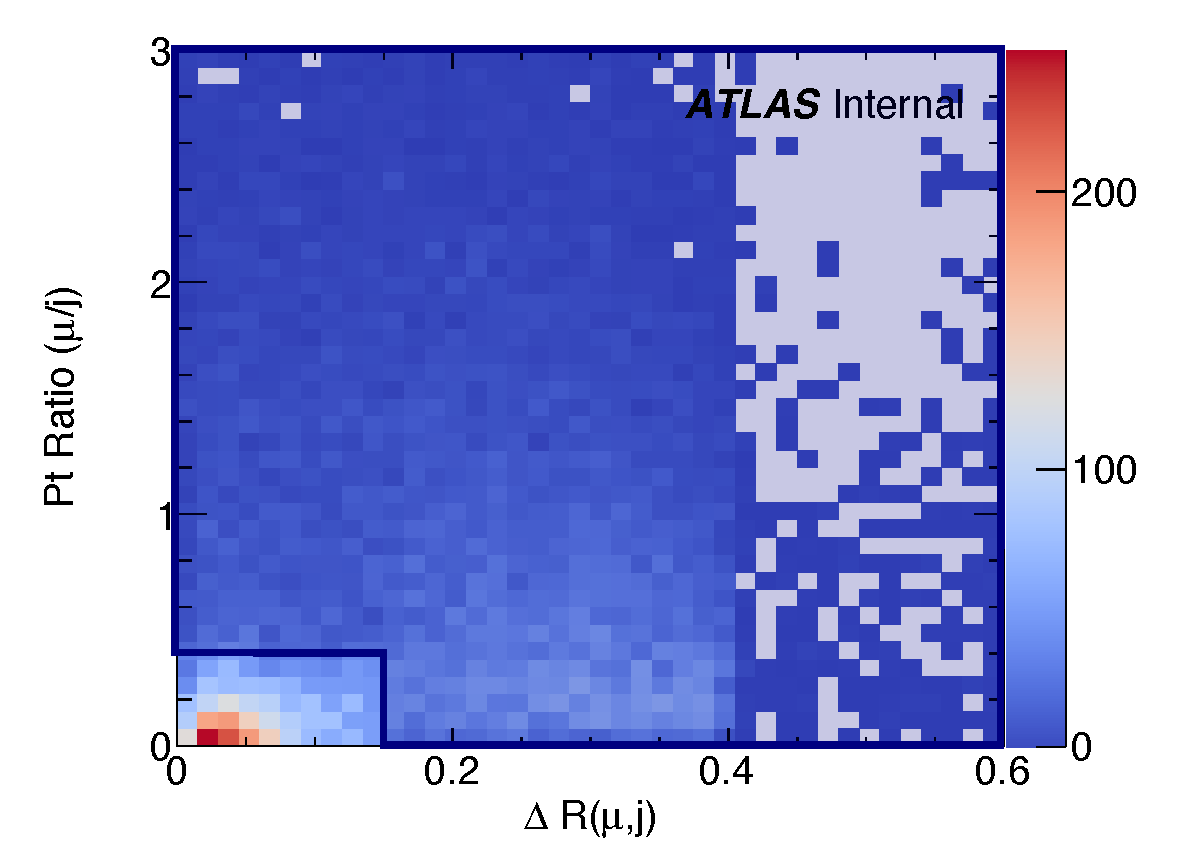
\includegraphics[width=.48\textwidth]{figs/ssww_13tev/custom_or/bkg_Muon_DR_PtRatio_edited}
  \caption{Stuff}
  \label{fig:ssww13tev_customor_muon_2d}
\end{figure}




\section{Cross section measurement}\label{ssww13tev:xsec}
Hello world!


\section{Summary of uncertainties}\label{ssww13tev:uncertainty}
Systematic uncertainties enter the final fit as nuisance parameters which can impact the estimated signal and background yields and the shapes of the $m_{jj}$ distributions.
These uncertainties can arise from the experimental methods or from the theoretical calculations used in the analysis.
This section summarizes the systematic uncertainties; the experimental uncertainties are detailed in Section~\ref{ssww13tev:experimental_uncert}, and the theoretical uncertainties are covered in Section~\ref{ssww13tev:theory_uncert}.
The impacts of the systematic uncertainties on the final cross section measurement are summarized in Table~\ref{tab:ssww13tev_total_uncert}.

\begin{table}[htbp]
  \centering
  \begin{tabular}{p{2ex}lc}
    \multicolumn{2}{l}{Source} & Impact [\%] \\
    \hline\hline
    \multicolumn{2}{l}{Reconstruction}           & ${\hphantom{0}\pm4.0}$ \\
    \hline
    & Electrons        & ${\hphantom{0}\pm0.5}$ \\
    & Muons            & ${\hphantom{0}\pm1.2}$ \\
    & Jets and $E_{\mathrm{T}}^{\mathrm{miss}}$ & ${\hphantom{0}\pm2.8}$ \\
    & $b$-tagging      & ${\hphantom{0}\pm2.0}$ \\
    & Pileup           & ${\hphantom{0}\pm1.5}$ \\
    \hline
    \multicolumn{2}{l}{Background}           & ${\hphantom{0}\pm5.0}$ \\
    \midrule
    & Misid.\ leptons  & ${\hphantom{0}\pm3.9}$ \\
    & Charge misrec.   & ${\hphantom{0}\pm0.3}$ \\
    & $WZ$             & ${\hphantom{0}\pm1.3}$ \\
    & \ssww QCD        & ${\hphantom{0}\pm2.8}$ \\
    & Other & ${\hphantom{0}\pm0.8}$ \\
    \hline
    \multicolumn{2}{l}{Signal}           & ${\hphantom{0}\pm3.6}$ \\
    \hline
    & Interference & ${\hphantom{0}\pm1.0}$ \\
    & EW Corrections & ${\hphantom{0}\pm1.3}$ \\
    & Shower, Scale, PDF \& $\alpha_s$ & ${\hphantom{0}\pm3.2}$ \\
    \hline
    \multicolumn{2}{l}{Total}            & ${\hphantom{0}\pm7.4}$ \\
    \hline
  \end{tabular}
  \caption{Impact of various systematic effects on the fiducial cross section measurement. The impact of a given source of uncertainty is computed by performing the fit with the corresponding nuisance parameter varied up or down by one standard deviation from its nominal value.}
  \label{tab:ssww13tev_total_uncert}    
\end{table}

\subsection{Experimental uncertainties}\label{ssww13tev:experimental_uncert}
Experimental uncertainties include detector effects as well as uncertainties on the background estimation methods.
Sources of systematic uncertainty on the measurement of physics objects are listed in Table~\ref{tab:ssww13tev_uncert_exp_uncert}, grouped by the relevant object type.
For backgrounds estimated from MC simulations, variations in these sources of uncertainty are propagated through the analysis to obtain the corresponding uncertainties on the event yields.
Additional experimental uncertainties include the integrated luminosity, the photon conversion rate from Section~\ref{ssww13tev:wgamma}, and the data driven charge misidentification and fake lepton background estimations from Sections~\ref{ssww13tev:charge_misid} and \ref{ssww13tev:ff_results}, respectively.

The largest sources of experimental uncertainty on the MC estimations come from the jet-related uncertainties and the $b$-tagging efficiency, while the largest uncertainty on the background estimation comes from the fake-factor.
The effects of the uncertainties on the \ssww EWK signal and the dominant MC estimated background, $WZ$, are listed in Tables~\ref{tab:ssww13tev_uncert_exp_wwewk} and \ref{tab:ssww13tev_uncert_exp_wz}, respectively.
Since the overall contributions from other processes estimated with MC are small, the uncertainties on these backgrounds have a lesser impact on the final measurement; these tables can be found in Appendix~\ref{app:ssww13tev_exp_uncert}.

\begin{table}[htbp]
  \centering
  \begin{tabular}{l | l}
    \multicolumn{2}{c}{Experimental uncertainties}\\
    \hline\hline
    \multirow{6}{*}{Electrons} & Energy resolution \\
    & Energy scale \\
    & Identification efficiency \\
    & Isolation efficiency \\
    & Reconstruction efficiency \\
    & Trigger efficiency \\
    \hline
    \multirow{5}{*}{Muons} & Energy scale \\
    & Identification efficiency  \\
    & Inner detector track resolution \\
    & Muon spectrometer resolution \\
    & Trigger efficiency \\
    \hline
    \multirow{2}{*}{$\met$} & Resolution \\
    & Scale \\
    \hline
    \multirow{5}{*}{Jets} & Energy resolution \\
    & Energy scale \\
    & JVT cut efficiency \\
    & $b$-tagging efficiency \\
    & Jets from pileup \\
    \hline
  \end{tabular}
  \caption{List of sources of experimental uncertainties on the reconstruction of physics objects.}
  \label{tab:ssww13tev_uncert_exp_uncert}
\end{table}

\begin{table}[htbp]
  \centering
  \begin{tabular}{l|ccc}
    \ssww EWK & $\ee$ \% Yield & $\me$ \% Yield & $\mm$ \% Yield \\
    \hline\hline
    Jet-related Uncertainties & \ensuremath{2.28} & \ensuremath{2.22} & \ensuremath{2.28}\\
    b-tagging efficiency & \ensuremath{1.81} & \ensuremath{1.76} & \ensuremath{1.74}\\
    Pile-up & \ensuremath{0.48} & \ensuremath{0.97} & \ensuremath{2.42}\\
    Trigger efficiency & \ensuremath{0.02} & \ensuremath{0.08} & \ensuremath{0.47}\\
    Lepton reconstruction/ID & \ensuremath{1.45} & \ensuremath{1.14} & \ensuremath{1.83}\\
    MET reconstruction & \ensuremath{0.26} & \ensuremath{0.17} & \ensuremath{0.21}\\
    \hline
  \end{tabular}
  \caption{Impact of experimental uncertainties for the \ssww EWK processes in all channels.}
  \label{tab:ssww13tev_uncert_exp_wwewk}
\end{table}

\begin{table}[htbp]
  \centering
  \begin{tabular}{l|ccc}
    $WZ$  & $\ee$ \% Yield & $\me$ \% Yield & $\mm$ \% Yield \\
    \hline\hline
    Jet-related Uncertainties & \ensuremath{9.58} & \ensuremath{5.03} & \ensuremath{8.45}\\
    b-tagging efficiency & \ensuremath{2.49} & \ensuremath{2.23} & \ensuremath{2.40}\\
    Pile-up & \ensuremath{2.99} & \ensuremath{3.49} & \ensuremath{3.33}\\
    Trigger efficiency & \ensuremath{0.03} & \ensuremath{0.09} & \ensuremath{0.43}\\
    Lepton reconstruction/ID & \ensuremath{1.52} & \ensuremath{1.24} & \ensuremath{3.07}\\
    MET reconstruction & \ensuremath{0.93} & \ensuremath{0.79} & \ensuremath{1.63}\\
    \hline
  \end{tabular}
  \caption{Impact of experimental uncertainties for the $WZ$ process in all channels.}
  \label{tab:ssww13tev_uncert_exp_wz}
\end{table}

\subsection{Theoretical uncertainties}\label{ssww13tev:theory_uncert}
It is also necessary to consider uncertainties on the theoretical predictions in the fiducial region.
They include the choice of PDF set, the value of the strong coupling constant $\alpha_s$, the renormalization scale $\mu_R$, the factorization scale $\mu_F$, and the parton showering.
The size of these uncertainties are measured by generating new samples with variations in a chosen parameters and comparing them to samples using the nominal choice of the parameter.
Internal variations on the PDF sets or using a different set entirely results in a relative uncertainty of up to $2.25\%$ on the nominal sample.
The impact from varying $\alpha_s$ is very small, on the order of $<0.01\%$.
The factorization and renormalization scales are independently varied between $0.5$-$2.0$ from their nominal values of $1.0$.
This results in relative uncertainties on the prediction of up to $15\%$.
Finally, varying the parameters in the parton showering results in up to $8\%$ uncertainty.
% mention NLO corrections? ~\cite{2017.ssww-nlo-corrections}

\subsubsection{Uncertainties from EWK-QCD interference}\label{ssww13tev:interference}
As mentioned in Section~\ref{ssww13tev:vbs_theory}, \ssww production consists of both EWK processes.
The two production modes cannot be naively separated due to cross terms in the matrix element calculation.
These cross terms are referred to as \emph{interference} terms.
Since the \ssww EWK production is the focus of the analysis, and the signal region is designed to preferentially select those events, it is important to measure the size of the EWK-QCD interference contributions.

The interference effects are estimated using the \tt{MadGraph} MC generator, as it has a feature that allows direct modelling of the interference term.
This allows four samples to be generated:
\begin{enumerate}
\item Inclusive: All available diagrams are used in the matrix element calculation
\item EWK only: Only EWK diagrams ($\mathcal{O}(\alpha_{\textrm{EWK}}) = 4$) are used
\item QCD only: Only QCD diagrams ($\mathcal{O}(\alpha_s) = 2 \otimes \mathcal{O}(\alpha_{\textrm{EWK}}) = 2$) are used
\item Interference: Only the interference terms are used
\end{enumerate}
A minimal set of generator level cuts, listed in Table~\ref{tab:ssww13tev_uncert_int_cuts}, is applied in order to avoid biasing the sample towards either production mode.
The cross sections for each of the four channels can be found in Table~\ref{tab:ssww13tev_uncert_int_xsec}
The size of the interference is found to be approximately $6\%$ of the total cross section and is taken as a systematic uncertainty.

\begin{table}[htbp]
  \centering
  \begin{tabular}{c}
    Generator level cuts\\
    \hline\hline
    $\Delta\eta_{jj} < 10$ \\
    Jet $\pt > 20\gev$ \\
    $M_{jj} > 10\gev$ \\
    \hline
  \end{tabular}
  \caption{The set of generator level cuts used for generating the interference samples with \tt{MadGraph}.}
  \label{tab:ssww13tev_uncert_int_cuts}
\end{table}

\begin{table}[htbp]
  \centering
  \begin{tabular}{l | c}
    Sample & $\sigma$ (fb) \\
    \hline\hline
    Inclusive    & $3.646\pm 0.0012$ \\
    EWK only     & $2.132\pm 0.0005$ \\
    QCD only     & $1.371\pm 0.0008$ \\
    Interference & $0.227\pm 0.0002$ \\
    \hline
  \end{tabular}
  \caption{Cross sections for each different \ssww production mode (inclusive, EWK only, QCD only, and interference only) generated using \tt{MadGraph}.  The cross sections are calculated using a minimal set of generator level cuts from events where the $W$ decays to a muon.}
  \label{tab:ssww13tev_uncert_int_xsec}
\end{table}


\section{Results}\label{ssww13tev:results}
%\TODO{Observed fit results: support note 9.7 p. 138}

After running the full analysis chain, the event yields in the signal region, low-$m_{jj}$ control region, and $WZ$ control region as well as associated nuisance parameters representing the uncertainties are passed to the maximum likelihood fit.
From this fit, the normalization factor for the $WZ$ control region $\mu_{WZ}$ and the signal strength parameter in the signal region $\mu_{\textrm{obs}}$ are determined, and the predicted yields in each input bin have been shifted according to the process detailed in Section~\ref{ssww13tev:xsec_fit_method}.

The $WZ$ normalization factor is measured to be:
\begin{equation}
  \mu_{WZ} = 0.88^{+0.07}_{-0.07}(\textrm{stat})~^{+0.31}_{-0.21}(\textrm{theory})~^{+0.22}_{-0.11}(\textrm{sys})
  \label{eq:ssww13tev_signal_strength_wz}
\end{equation}
and is constrained primarily by the number of data events in the $WZ$ control region.
The observed signal strength of \ssww EWK production, defined in Equation~\ref{eq:ssww13tev_xsec_mu}, is extracted from the fit and measured with respect to the prediction of the \sherpav{2.2.2} MC generator:
\begin{equation}
  \mu_{\textrm{obs}} = 1.45^{+0.25}_{-0.24}(\textrm{stat})~^{+0.06}_{-0.08}(\textrm{theory})~^{+0.27}_{-0.22}(\textrm{sys}) % paper has no theory uncert for some reason
  \label{eq:ssww13tev_signal_strength_sr}
\end{equation}
This corresponds to a rejection of the background-only hypothesis with a significance of $6.9\sigma$.

The observed number of data events are compared to the predicted signal and background yields in the signal region in Table~\ref{tab:ssww13tev_yields_prefit} before applying the fit and in Table~\ref{tab:ssww13tev_yields_postfit} after the fit.
The $m_{jj}$ distributions for data and prediction are shown in Figure~\ref{fig:ssww13tev_results_mjj_sr_postfit} after the fit, and the fitted event yields in the low-$m_{jj}$ and $WZ$ control regions are shown in Figure~\ref{fig:ssww13tev_results_cr_postfit}.
Additional distributions can be found in Appendix~\ref{app:ssww13tev_additional_material}.

\begin{table}[htbp]
  \resizebox{\linewidth}{!}{
  \begin{tabular}{l|l@{$\,\pm\,$}ll@{$\,\pm\,$}ll@{$\,\pm\,$}ll@{$\,\pm\,$}ll@{$\,\pm\,$}ll@{$\,\pm\,$}l|l@{$\,\pm\,$}l}
    & \multicolumn{2}{c}{$\eep$}& \multicolumn{2}{c}{$\eem$}& \multicolumn{2}{c}{$\mep$}& \multicolumn{2}{c}{$\mem$}& \multicolumn{2}{c}{$\mmp$}& \multicolumn{2}{c|}{$\mmm$}& \multicolumn{2}{c}{combined}\\
\hline\hline
$WZ$                    & 1.9 & 0.6 & 1.3 & 0.4 & 14 & 4 & 8.9 & 2.6 & 5.5 & 1.6 & 3.6 & 1.1 & 35 & 10 \\ % before scaling (calculated by hand)
Non-prompt            & 4.1& 2.3   & 2.3& 1.7   & 9& 5   & 6& 4   & 0.57& 0.15   & 0.67& 0.25   & 23& 10 \\
$e/\gamma$ conversions         & 1.74& 0.29   & 1.8& 0.4   & 6.1& 1.6   & 3.7& 0.8   & \multicolumn{2}{c}{---}   & \multicolumn{2}{c|}{---}   & 13.4& 2.5 \\
Other prompt          & 0.17& 0.05   & 0.14& 0.04   & 0.90& 0.19   & 0.60& 0.14   & 0.36& 0.10   & 0.19& 0.05   & 2.4& 0.5 \\
\ssww QCD              & 0.38& 0.13   & 0.16& 0.05   & 3.0& 1.0   & 1.2& 0.4   & 1.8& 0.6   & 0.76& 0.25   & 7.3& 2.5 \\
\hline
Expected background   & 8.2 & 2.4 & 5.7 & 1.8 & 33 & 7 & 21 & 5 & 8.2 & 1.8 & 5.3 & 1.2 & 81 & 14  \\
\hline
\ssww EWK & 3.8 & 0.6 & 1.49 & 0.22 & 16.5 & 2.5 & 6.5 & 1.0 & 9.1 & 1.4 & 3.5 & 0.5 & 41 & 6 \\
\hline
Data& \multicolumn{2}{c}{10}& \multicolumn{2}{c}{4}& \multicolumn{2}{c}{44}& \multicolumn{2}{c}{28}& \multicolumn{2}{c}{25}& \multicolumn{2}{c|}{11}& \multicolumn{2}{c}{122}\\
\hline
\end{tabular}
  }
  \caption{Table of the data and prediction event yields in the signal region before the fit.  Numbers are shown for the six lepton flavor and charge channels and for all channels combined.  Here the $WZ$ background yields are normalized to the data in the $WZ$ control region.  The background estimations from the fake factor are included in the ``Non-prompt'' category, and backgrounds from  $V\gamma$ production and electron charge misidentification are combined in the ``$e/\gamma$ conversions'' category. Finally, $ZZ$, $VVV$, and $t\bar{t}V$ backgrounds are combined in the ``Other prompt'' category.}
  \label{tab:ssww13tev_yields_prefit}
\end{table}

\begin{table}[htbp]
  \resizebox{\linewidth}{!}{
    \begin{tabular}{l|l@{$\,\pm\,$}ll@{$\,\pm\,$}ll@{$\,\pm\,$}ll@{$\,\pm\,$}ll@{$\,\pm\,$}ll@{$\,\pm\,$}l|l@{$\,\pm\,$}l}
    & \multicolumn{2}{c}{$\eep$}& \multicolumn{2}{c}{$\eem$}& \multicolumn{2}{c}{$\mep$}& \multicolumn{2}{c}{$\mem$}& \multicolumn{2}{c}{$\mmp$}& \multicolumn{2}{c|}{$\mmm$}& \multicolumn{2}{c}{combined}\\
    \hline\hline
    $WZ$                    & 1.49& 0.30   & 1.10& 0.26   & 11.7& 1.7   & 8.0& 1.3   & 5.0& 0.6   & 3.5& 0.6   & 31& 4 \\
    Non-prompt            & 2.2& 1.3   & 1.2& 0.7   & 5.7& 2.8   & 4.5& 1.8   & 0.57& 0.06   & 0.65& 0.14   & 15& 6 \\
    $e/\gamma$ conversions           & 1.6& 0.4   & 1.6& 0.5   & 6.3& 1.6   & 4.3& 1.1   & \multicolumn{2}{c}{---} & \multicolumn{2}{c|}{---}   & 13.8& 2.9 \\
    Other prompt          & 0.16& 0.04   & 0.14& 0.04   & 0.90& 0.19   & 0.63& 0.13   & 0.39& 0.09   & 0.22& 0.05   & 2.4& 0.5 \\
    \ssww QCD              & 0.35& 0.13   & 0.15& 0.05   & 2.9& 1.0   & 1.2& 0.4   & 1.8& 0.6   & 0.76& 0.25   & 7.2& 2.4 \\
    \hline
    Expected background   & 5.8& 1.5   & 4.1& 1.1   & 27& 4   & 18.7& 2.6   & 7.7& 0.8   & 5.1& 0.6   & 69& 7 \\
    \hline
    \ssww EWK            & 5.6& 1.0   & 2.2& 0.4   & 24& 5   & 9.4& 1.8   & 13.5& 2.5   & 5.2& 1.0   & 60& 11 \\
    \hline
    Data& \multicolumn{2}{c}{10}& \multicolumn{2}{c}{4}& \multicolumn{2}{c}{44}& \multicolumn{2}{c}{28}& \multicolumn{2}{c}{25}& \multicolumn{2}{c|}{11}& \multicolumn{2}{c}{122}\\
    \hline
    \end{tabular}
  }
  \caption{Table of the data and prediction event yields in the signal region after the fit.  Numbers are shown for the six lepton flavor and charge channels and for all channels combined.  The background estimations from the fake factor are included in the ``Non-prompt'' category, and backgrounds from  $V\gamma$ production and electron charge misidentification are combined in the ``$e/\gamma$ conversions'' category.  Finally, $ZZ$, $VVV$, and $t\bar{t}V$ backgrounds are combined in the ``Other prompt'' category.}
  \label{tab:ssww13tev_yields_postfit}
\end{table}

\begin{figure}[htbp]
  \centering
  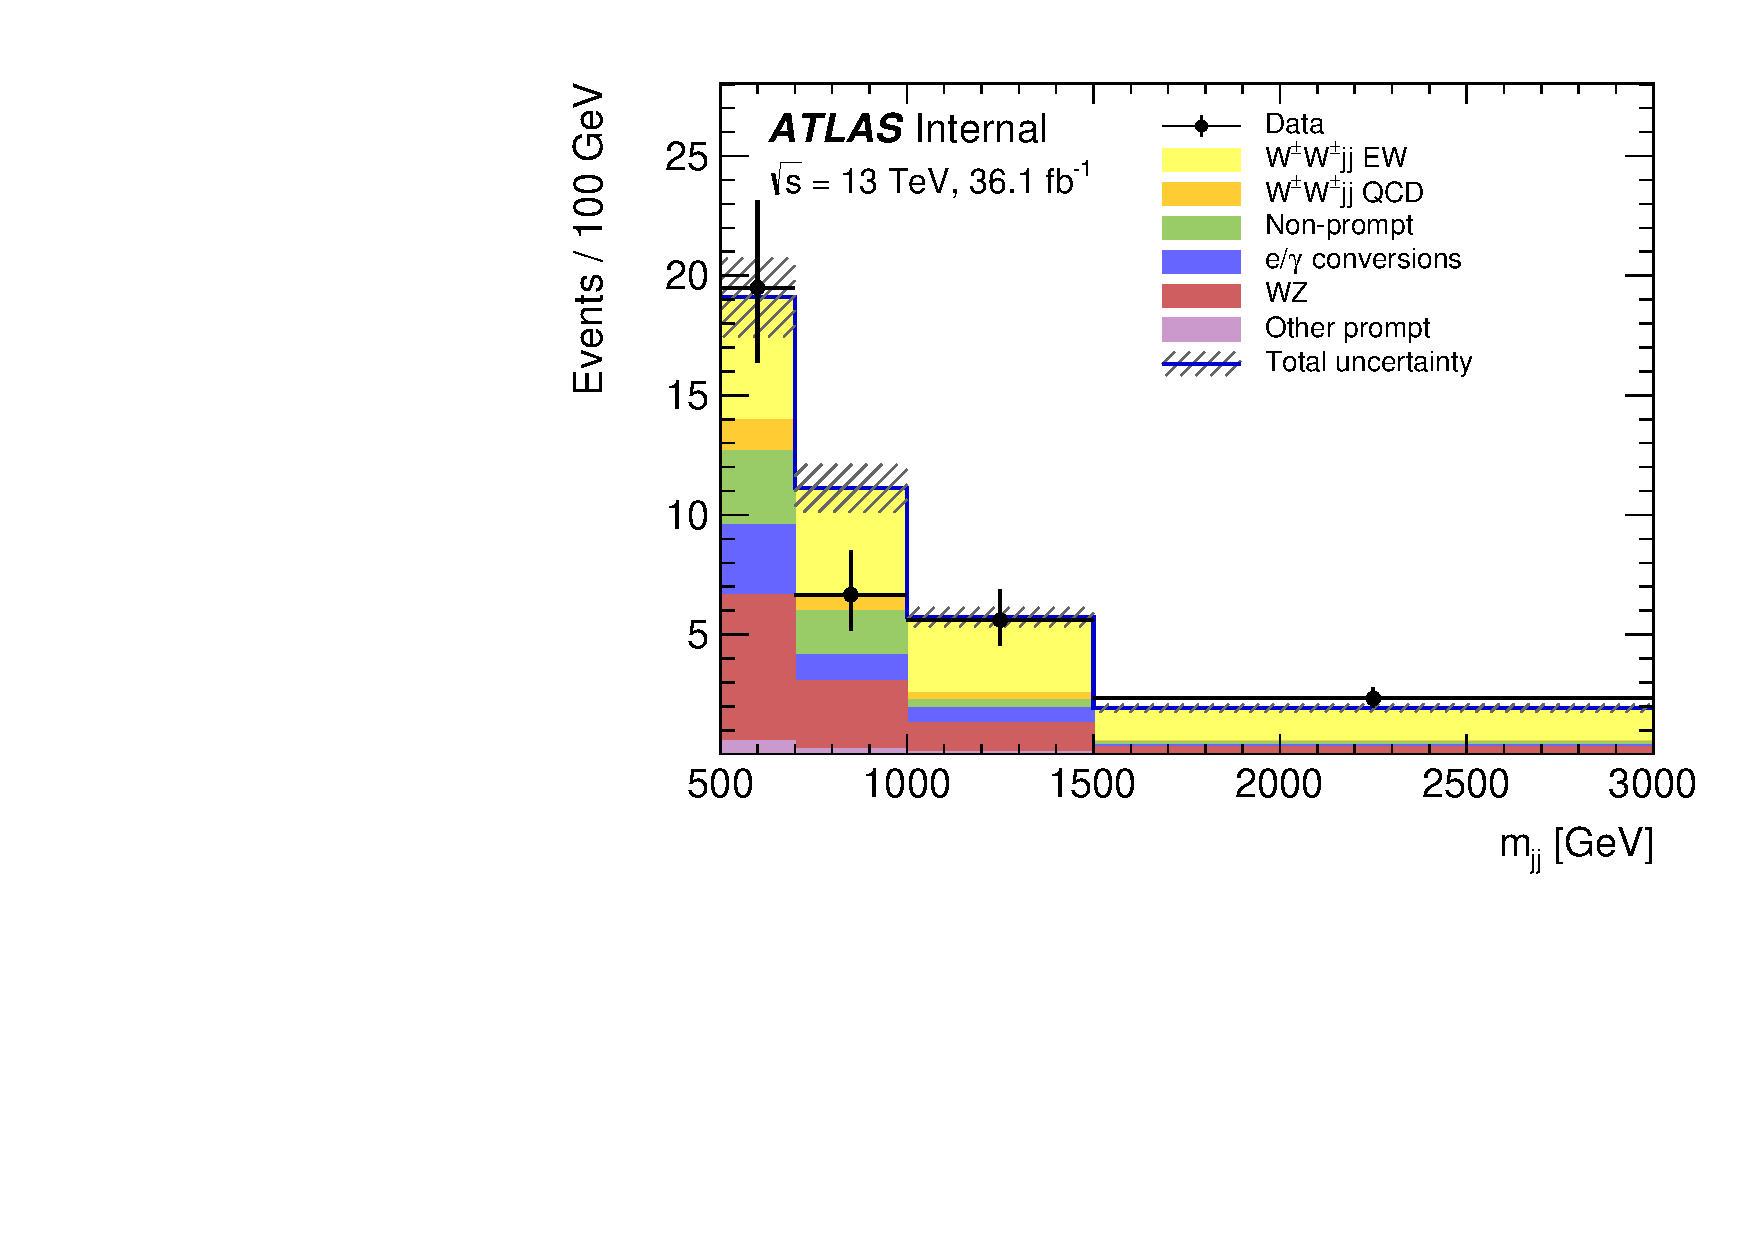
\includegraphics[width=.6\textwidth]{figs/ssww_13tev/results/mjj_postfit_all}
  \caption{The dijet invariant mass $m_{jj}$ distributions for data and predicted signal and background in the signal region after the fit.  The shaded band represents the statistical and systematic uncertainties added in quadrature.  Note that the bins have been scaled such that they represent the number of events per $100\gev$ in $m_{jj}$.  The background estimations from the fake factor are included in the ``Non-prompt'' category, and backgrounds from  $V\gamma$ production and electron charge misidentification are combined in the ``$e/\gamma$ conversions'' category.  Finally, $ZZ$, $VVV$, and $t\bar{t}V$ backgrounds are combined in the ``Other prompt'' category.}
  \label{fig:ssww13tev_results_mjj_sr_postfit}
\end{figure}

\begin{figure}[htbp]
  \centering
  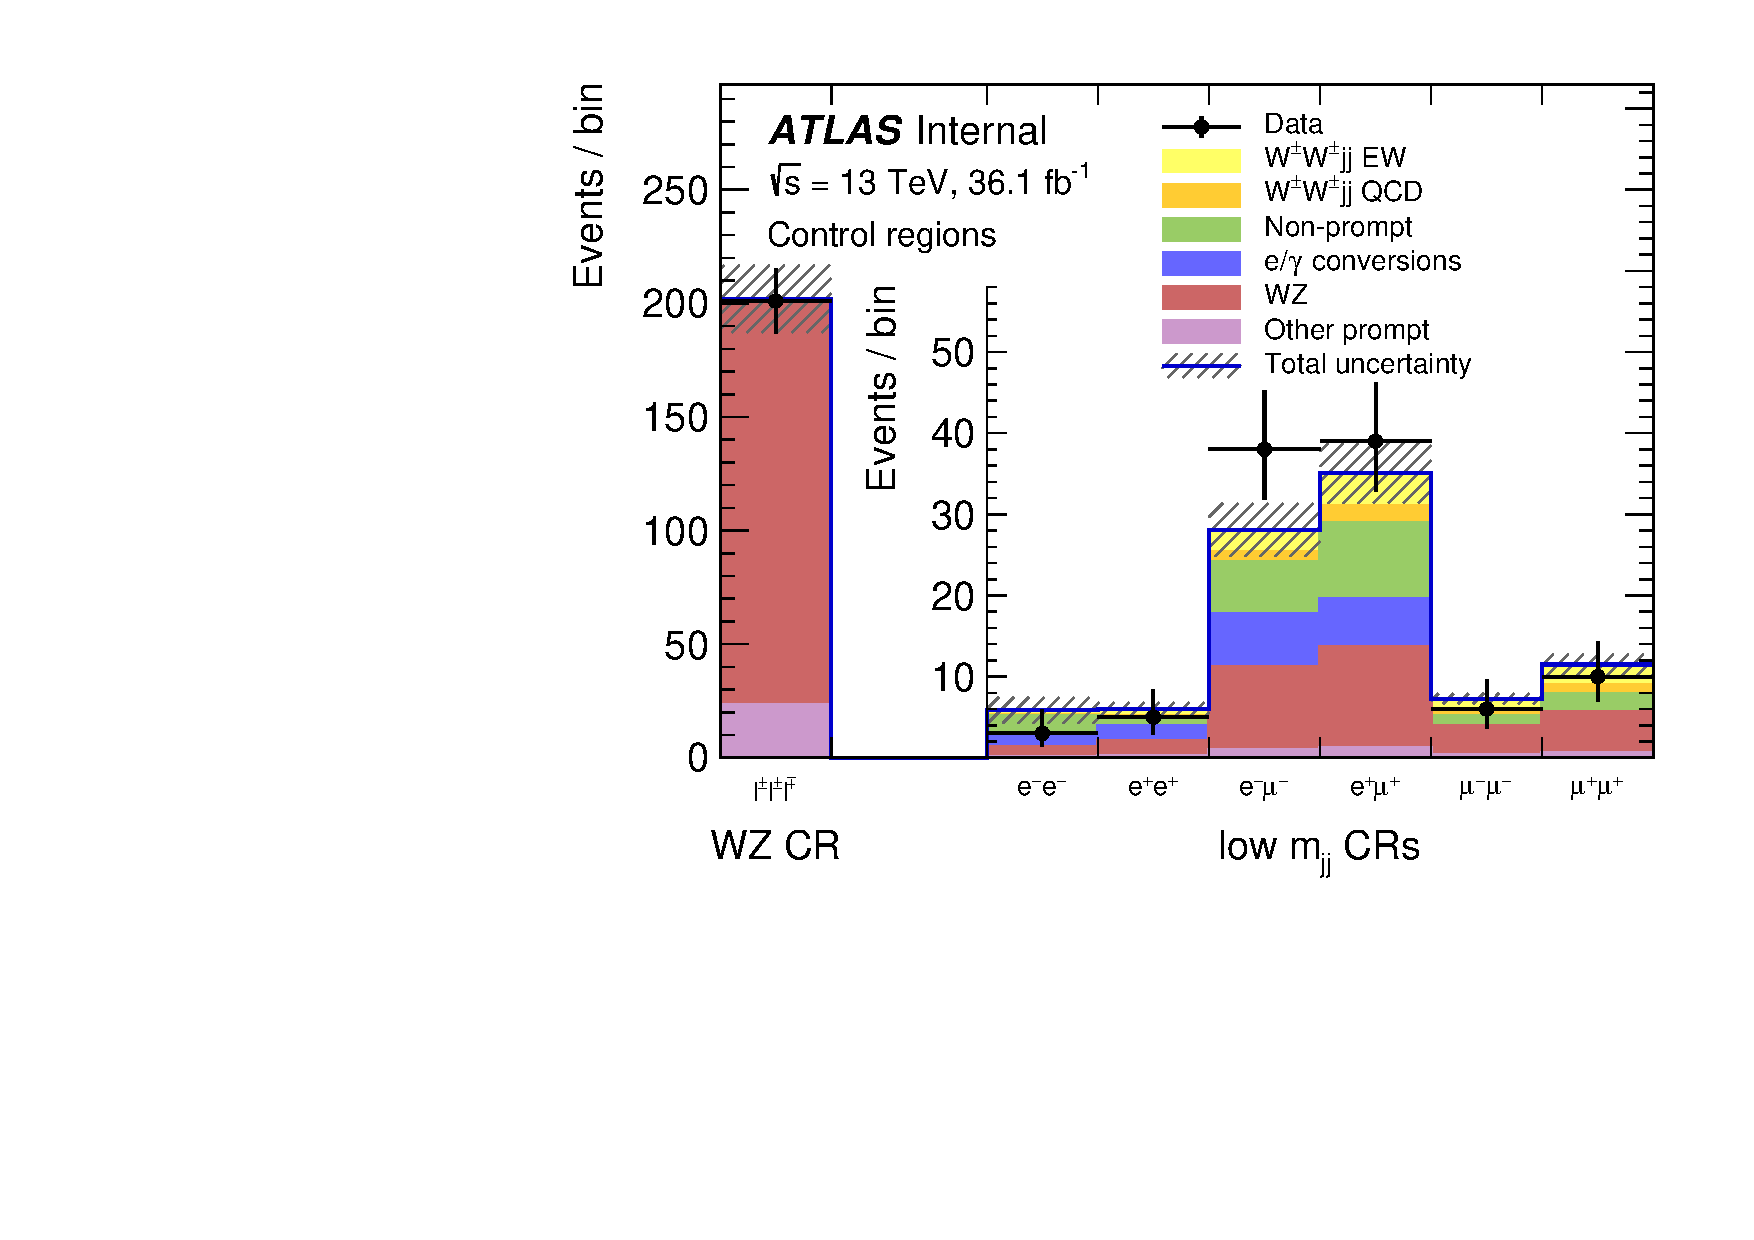
\includegraphics[width=.6\textwidth]{figs/ssww_13tev/results/plotCR}
  \caption{The event yields for data and predicted signal and background in the $WZ$ and low-$m_{jj}$ control regions after the fit.  The shaded band represents the statistical and systematic uncertainties added in quadrature.  The background estimations from the fake factor are included in the ``Non-prompt'' category, and backgrounds from  $V\gamma$ production and electron charge misidentification are combined in the ``$e/\gamma$ conversions'' category.  Finally, $ZZ$, $VVV$, and $t\bar{t}V$ backgrounds are combined in the ``Other prompt'' category.}
  \label{fig:ssww13tev_results_cr_postfit}
\end{figure}

The last ingredient necessary to measure the \ssww EWK cross section is the theory predicted cross section in the fiducial region defined in Table~\ref{tab:ssww13tev_fiducial_vol}.
\sherpav{2.2.2} is used for the calculation, and the cross section in the total generator phase space is $40.81\pm 0.05~\textrm{fb}$, and the fiducial cross section is $2.01\pm 0.02~\textrm{fb}$.
This corresponds to an acceptance factor of $\mathcal{A} = 0.0493\pm 0.0002$.
Uncertainties on the simulation are estimated using variations of the scale, parton shower, and PDF set.
The final prediction used in the cross section measurement including uncertainties from Section~\ref{ssww13tev:theory_uncert} is:
\begin{equation}
  \sigma_{\tt{SHERPA}}^{\textrm{fid}} = 2.01 \pm 0.02(\textrm{stat})~^{+0.29}_{-0.23} (\textrm{scale})~^{+0.16}_{-0.02}(\textrm{parton shower})~^{+0.05}_{-0.03} (\textrm{PDF})~\textrm{fb}
  \label{eq:ssww13tev_fiducial_xsec_theory}
\end{equation}

Combining this \tt{SHERPA} prediction with the measured signal strength $\mu_{\textrm{obs}}$ from Equation~\ref{eq:ssww13tev_signal_strength_sr}, the measured fiducial cross section $\sigma_{\textrm{meas}}^{\textrm{fid}}$ can be calculated using Equation~\ref{eq:ssww13tev_xsec_fid_meas_mu}:
\begin{equation}
  \sigma_{\textrm{meas}}^{\textrm{fid}} = 2.91^{+0.51}_{-0.47}(\textrm{stat})~^{+0.12}_{-0.16}(\textrm{theory})~^{+0.24}_{-0.23}(\textrm{sys})~^{+0.08}_{-0.06}(\textrm{luminosity})~\textrm{fb}
  \label{eq:ssww13tev_fiducial_xsec}
\end{equation}
A plot comparing the measured fiducial cross section to two theoretical calculations is shown in Figure~\ref{fig:ssww13tev_results_xsec}.
The measured value is compared to the \sherpav{2.2.2} prediction used to calculate $\mu_{\textrm{obs}}$ as well as to \powhegbox{2}.
As mentioned in Section~\ref{ssww13tev:mc}, this \tt{POWHEG} sample does not include the resonant triboson diagrams and is only used here for a visual comparison.

\begin{figure}[htbp]
  \centering
  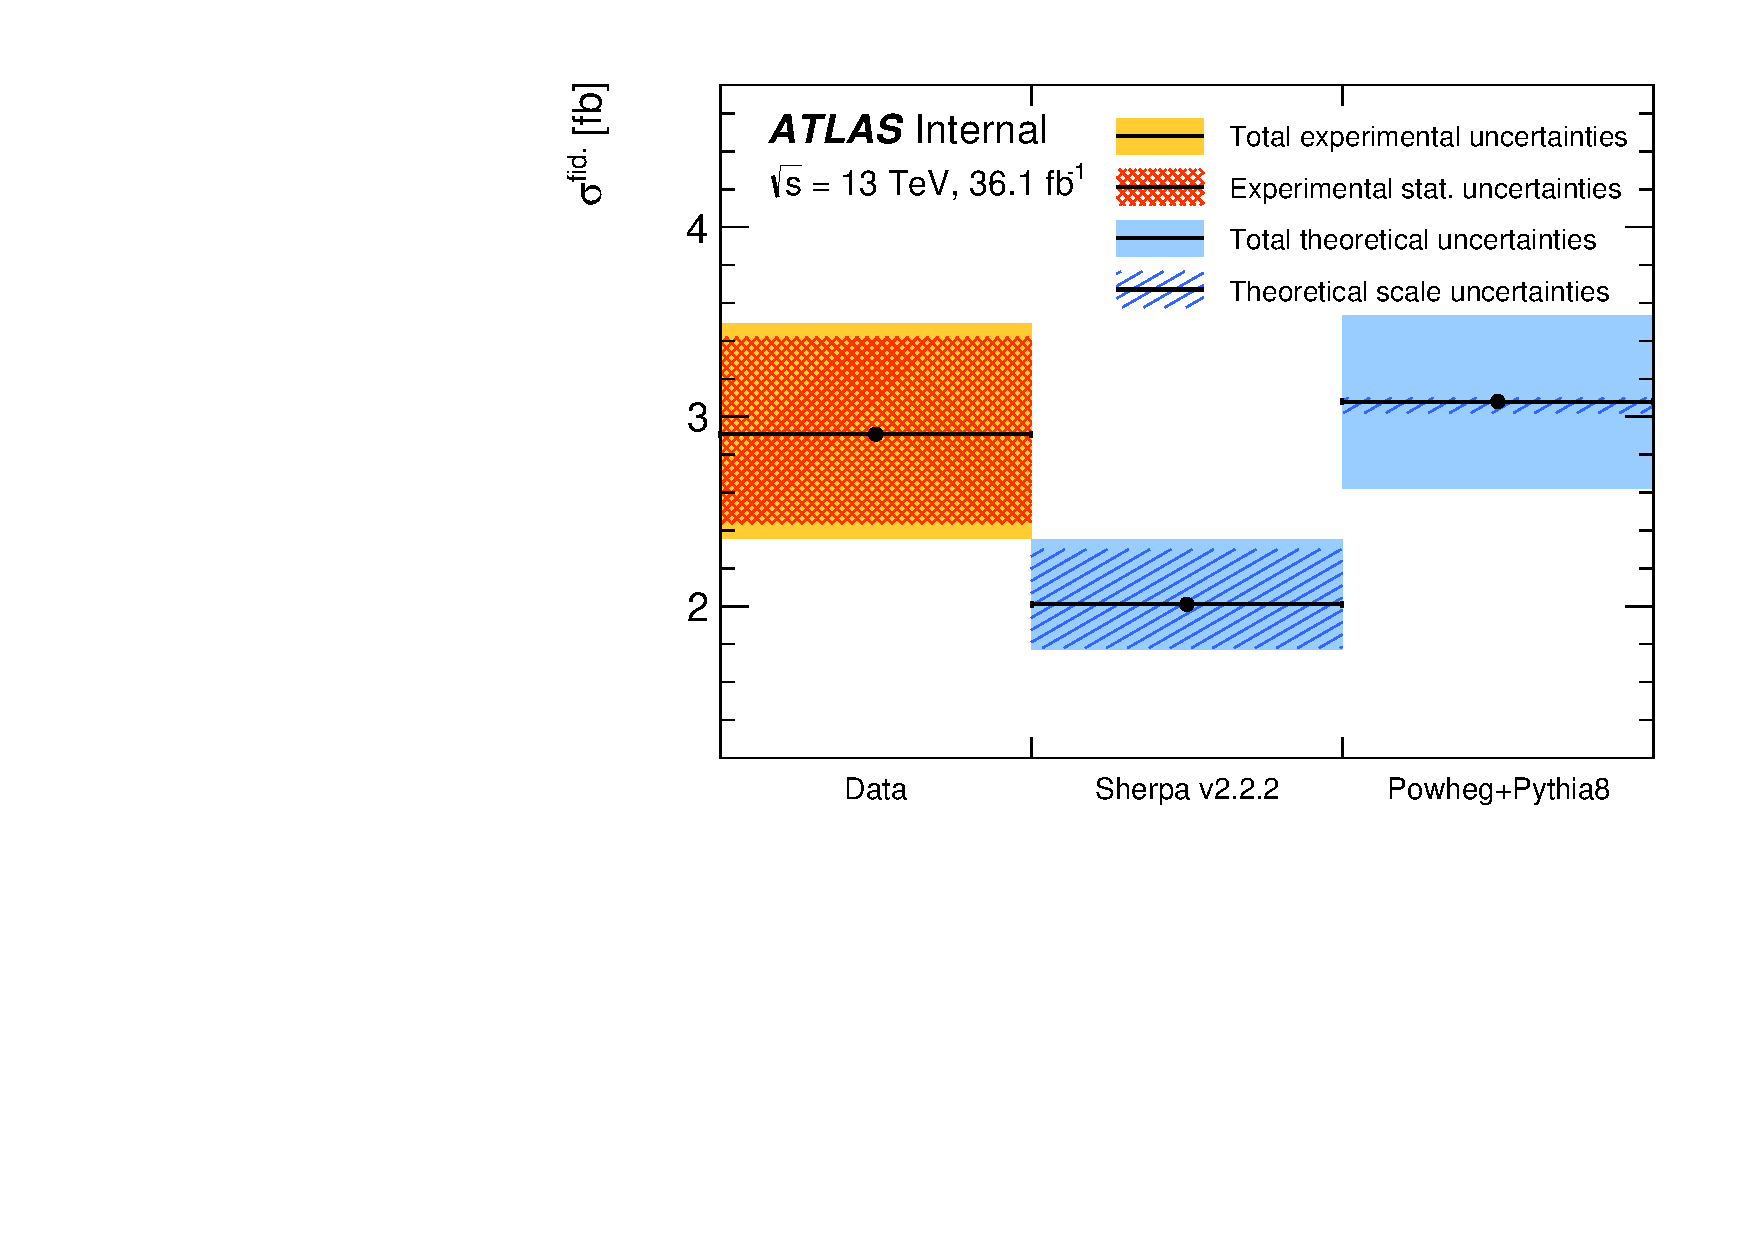
\includegraphics[width=.6\textwidth]{figs/ssww_13tev/results/NP_post_fit__xsec_ExpObs}
  \caption{Comparison of the measured \ssww EWK fiducial cross section with theoretical calculations from \sherpav{2.2.2} and \powhegbox{2}.  The light orange band represents the total experimental uncertainty on the measured value, and the dark orange hashed band is the statistical uncertainty.  For the simulations, the light blue band represents the total theoretical uncertainty, and the dark blue hashed band are the scale uncertainties.  The theory predictions do not include the interference between the EWK and QCD production.}
  \label{fig:ssww13tev_results_xsec}
\end{figure}


\subsection{Beyond the Standard Model extensions of \ssww}\label{ssww13tev:extensions}
Many so-called \emph{Beyond the Standard Model} (BSM) theories exist that incorporate new physics with what has been experimentally observed.
BSM theories often manifest as deviations from the expected SM cross sections, either due to additional decay possibilities affecting branching ratios or modifications of the coupings themselves.
One of the most well-known avenues for BSM involving new particles is supersymmetry~\cite{1997.susy-primer}; however, two popular BSM extensions relevant to the \ssww process involve a doubly-charged Higgs particle ($H^{\pm\pm}$) and anomalous triple and quartic gauge couplings (aQGC and aTGC, respectively)\footnote{The aQGC's are the focus in this section since the $WWWW$ QGC vertex is accessible through \sswwnojj scattering, as well as the fact that aTGC's have been studied in far greater detail due to being accessibile through a larger number of processes.}.
These two BSM theories will be touched on in the context of \ssww analyses at the LHC.

\subsubsection{Doubly charged Higgs bosons}\label{ssww13tev:hpp}
\cite{1985.doubly-charged-higgs, 2013.triplet-higgs-lhc}

\subsubsection{Anomalous quartic couplings}\label{ssww13tef:aqgc}
In the event that new physics exists at an energy scale far above what is currently accessible at the LHC, it cannot be directly observed by the experiment; however, its effects can still appear in the interactions between known particles.
In this case, the SM is simply the low-energy behavior of a larger \emph{effective field theory} (EFT), which contains additional, higher-dimensional operators that obey the existing SM symmetries:
\begin{equation}
  \mathcal{L}_{EFT} = \mathcal{L}_{SM}+\sum\limits_{d > 4}\sum\limits_i \frac{\tilde{c}_{i}}{\Lambda^{d-4}}\mathcal{O}_{i}
  \label{eq:eft_lagrangian}
\end{equation}
where $\mathcal{O}_i$ are operators of dimension $d$ with coefficients $\tilde{c}_i$, and $\Lambda$ is the energy scale of the new physics.
Here it can be clearly seen that as the energy scale $\Lambda\rightarrow\infty$, the SM behavior dominates.
In the region where $E\muchless\Lambda$, operators with high dimensionality contribute less to the total Lagrangian, and the summation may be truncated above a chosen value of $d$, at which point $\mathcal{L}_{EFT}$ becomes predictive and can parametrize any heavy new physics~\cite{2013.aqgc-mc}.

%EFT models are appealing due to the fact that they use the existing fields and symmetries of the SM and are consistent with existing SM results (since there is no current evidence for new physics) in the $\Lambda\rightarrow\infty$ limit.
%In this limit, these operators' contributions to observables can be estimated perturbatively in $(E/\Lambda)$~\cite{2017.multiboson-at-lhc}.
%The EFT can be written in terms of the SM Lagrangian plus contributions from operators $\mathcal{O}$ of dimension $\Delta$:

Only operators with even dimensionality are allowed in order to conserve baryon and lepton numbers.
The largest contributions to $\mathcal{L}_{EFT}$ therefore come from operators with $d=6$; however, any of these operators which modify the QGC's also modify the TGC's.
As a result, these operators are better constrained by existing analyses with greater sensitivity to TGC's.
Operators with $d=8$ are the lowest that modify exclusively the QGC's, of which there are 18, and nine of them modify the $WWWW$ QGC accessible through same-sign \sswwnojj scattering~\cite{2006.aqgc-at-lhc, 2013.aqgc-mc}:
\begin{equation}
  \begin{aligned}
    &\mathcal{O}_{S,0} = \big[(D_\mu\Phi)^\dagger D_\nu\Phi\big]\times\big[(D^\mu\Phi)^\dagger D^\nu\Phi\big]\\
    &\mathcal{O}_{S,1} = \big[(D_\mu\Phi)^\dagger D^\mu\Phi\big]\times\big[(D_\nu\Phi)^\dagger D^\nu\Phi\big]\\
    &\mathcal{O}_{M,0} = \textrm{Tr}\big[\hat{W}_{\mu\nu}\hat{W}^{\mu\nu}\big]\times\big[(D_\beta\Phi)^\dagger D^\beta\Phi\big]\\
    &\mathcal{O}_{M,1} = \textrm{Tr}\big[\hat{W}_{\mu\nu}\hat{W}^{\nu\beta}\big]\times\big[(D_\beta\Phi)^\dagger D^\mu\Phi\big]\\
    &\mathcal{O}_{M,6} = \big[(D_\mu\Phi)^\dagger\hat{W}_{\beta\nu}\hat{W}^{\beta\nu}D^\mu\Phi\big]\\
    &\mathcal{O}_{M,7} = \big[(D_\mu\Phi)^\dagger\hat{W}_{\beta\nu}\hat{W}^{\beta\mu}D^\nu\Phi\big]\\
    &\mathcal{O}_{T,0} = \textrm{Tr}\big[\hat{W}_{\mu\nu}\hat{W}^{\mu\nu}\big]\times\textrm{Tr}\big[\hat{W}_{\alpha\beta}\hat{W}^{\alpha\beta}\big]\\
    &\mathcal{O}_{T,1} = \textrm{Tr}\big[\hat{W}_{\alpha\nu}\hat{W}^{\mu\beta}\big]\times\textrm{Tr}\big[\hat{W}_{\mu\beta}\hat{W}^{\alpha\nu}\big]\\
    &\mathcal{O}_{T,2} = \textrm{Tr}\big[\hat{W}_{\alpha\mu}\hat{W}^{\mu\beta}\big]\times\textrm{Tr}\big[\hat{W}_{\beta\nu}\hat{W}^{\nu\alpha}\big]\\
  \end{aligned}
  \label{eq:aqgc_dim8}
\end{equation}
Each operator is paired with a coupling in the Lagrangian term: $\mathcal{L}_{S,0} = \frac{f_{S,0}}{\Lambda^4}\mathcal{O}_{S,0}$ and so on.
The SM prediction can be compared to simulations generated with chosen values for the anomalous coupling constants, as shown in Figure~\ref{fig:ssww13tev_aqgc}.

\begin{figure}
  \centering
  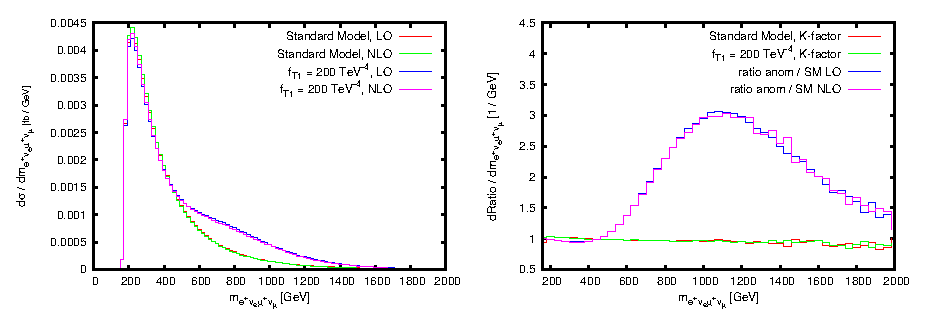
\includegraphics[width=.95\textwidth]{figs/ssww_13tev/extensions/aqgc}
  \caption[Invariant mass distributions of the $2l2\nu$ system in $pp\rightarrow e^{+}\nu_{e}\mu^{+}\nu_{\mu}jj$ events at LO and NLO with the \tt{VBFNLO} MC generator.  SM predictions are compared to those with the anomalous coupling $\frac{f_{T,1}}{\Lambda^4} = 200\tev^{-4}$.  The left plot shows the differential cross section for each prediction, and the right plot shows the $K$-factors for the SM and anomalous coupling predictions as well as the cross section ratio between the anomalous coupling and SM predictions at LO and NLO.]{Invariant mass distributions of the $2l2\nu$ system in $pp\rightarrow e^{+}\nu_{e}\mu^{+}\nu_{\mu}jj$ events at LO and NLO with the \tt{VBFNLO} MC generator.  SM predictions are compared to those with the anomalous coupling $\frac{f_{T,1}}{\Lambda^4} = 200\tev^{-4}$.  The left plot shows the differential cross section for each prediction, and the right plot shows the $K$-factors for the SM and anomalous coupling predictions as well as the cross section ratio between the anomalous coupling and SM predictions at LO and NLO.  Plots taken from~\cite{2013.aqgc-mc}.}
  \label{fig:ssww13tev_aqgc}
\end{figure}

Limits on the anomalous couplings generated by the $d=8$ operators of Equation~\ref{eq:aqgc_dim8} have been set by CMS in their \ssww analyses at $\sqrt{s} = 8\textrm{\ and\ }13\tev$~\cite{2015.ssww-8tev-cms, 2017.ssww-13tev-cms}.
ATLAS has also set limits at \com{8}~\cite{2014.ssww-8tev-atlas} using a different parameterization of the anomalous couplings outlined in~\cite{2013.aqgc-alpha}.
The limits set in CMS's $13\tev$ analysis are reproduced in Table~\ref{tab:aqgc_cms}.
The limits are obtained from fits to the $m_{ll}$ distributions in the signal and $WZ$ control regions, and 95\% confidence intervals are calculated by varying each operator individually.

\begin{table}[htbp]
  \centering
  \begin{tabular}{l c}
    Coupling & Observed limits $[\textrm{TeV}^{-4}]$ \\
    \hline\hline
    $f_{S,0}/\Lambda^4$ & $[-7.7, 7.7]$ \\
    $f_{S,1}/\Lambda^4$ & $[-21.6, 21.8]$ \\
    $f_{M,0}/\Lambda^4$ & $[-6.0, 5.9]$ \\
    $f_{M,1}/\Lambda^4$ & $[-8.7, 9.1]$ \\
    $f_{M,6}/\Lambda^4$ & $[-11.9, 11.8]$ \\
    $f_{M,7}/\Lambda^4$ & $[-13.3, 12.9]$ \\
    $f_{T,0}/\Lambda^4$ & $[-0.62, 0.65]$ \\
    $f_{T,1}/\Lambda^4$ & $[-0.28, 0.31]$ \\
    $f_{T,2}/\Lambda^4$ & $[-0.89, 1.02]$ \\
    \hline
  \end{tabular}
  \caption[Observed 95\% confidence limits set by CMS at \com{13} on the nine dimension-eight operators that modify the $WWWW$ QGC listed in Equation~\ref{eq:aqgc_dim8}.]{Observed 95\% confidence limits set by CMS at \com{13} on the nine dimension-eight operators that modify the $WWWW$ QGC listed in Equation~\ref{eq:aqgc_dim8}. Table taken from~\cite{2017.ssww-13tev-cms}.}
  \label{tab:aqgc_cms}
\end{table}

